% !Mode:: "TeX:UTF-8"
% !TEX program  = xelatex
% !BIB program  = biber
\documentclass[AutoFakeBold,AutoFakeSlant,language=english,degree=bachelor,zihao=-4]{sustechthesis}
% 1. AutoFakeBold 与 AutoFakeSlant 为伪粗与伪斜,如果本机上有相应粗体与斜体字体,请使用 xeCJK 宏包进行设置,例如:
%   \setCJKmainfont[
%     UprightFont = * Light,
%     BoldFont = * Bold,
%     ItalicFont = Kaiti SC,
%     BoldItalicFont = Kaiti SC Bold,
%   ]{Songti SC}
%
% 2. language=chinese 基于为 ctexart 文类提供的中文排版方案修改,如果使用英文进行论文创作,请使用 language=english 选项。
%
% 3. degree=bachelor 为 sustechthesis 文类提供的本科生毕业论文模板,其他可选项为 master 与 doctor,但是均未实现,如果您对此有兴趣,欢迎 PR。
%
% 4. sustechthesis.cls 文类主要参考自去年完成使命的 sustechthesis.tex,在这一年的时间,作者的 TeX 风格与常用宏包发生许多变化,因为之前的思想为仅提供必要的格式修改相关代码,所以转换为文类形式所进行的修改较少,而近期的风格与常用宏包均体现在以下的例子文件中。
%
% 5. 示例文件均放置于相应目录的 examples 文件夹下,构建自己论文时可暂时保留,用以检索接口与使用方法。
%
% 6. 英文目录需要居中可以使用:\renewcommand{\contentsname}{\centerline{Content}}
%
% 7. LaTeX 中公式编号括号样式及章节关联的方法:https://liam.page/2013/08/23/LaTeX-Formula-Number/

% !Mode:: "TeX:UTF-8"
% !TEX program  = xelatex

% 数学符号与环境
\usepackage{amsmath,amssymb}
  \newcommand{\dd}{\mathrm{d}}
  \newcommand{\RR}{\mathbb{R}}
  \newtheorem{definition}{Definition}
  \newtheorem{problem}{Problem}
% 参考文献
\usepackage[sorting=none, style=gb7714-2015, gbpub=false, gbpunctin=true, gbnamefmt=lowercase, backend=biber]{biblatex}
  \addbibresource{ref.bib}
% 无意义文本
\usepackage{zhlipsum,lipsum}
% 列表环境设置
\usepackage{enumitem}
% 浮动题不越过 \section
\usepackage[section]{placeins}
% 超链接
\usepackage{hyperref}
% 图片,子图,浮动题设置
\usepackage{graphicx,subcaption,float}
% 抄录环境设置,更多有趣例子请命令行输入 `texdoc tcolorbox`
\usepackage{tcolorbox}
  \tcbuselibrary{xparse}
  \DeclareTotalTCBox{\verbbox}{ O{green} v !O{} }%
    {fontupper=\ttfamily,nobeforeafter,tcbox raise base,%
    arc=0pt,outer arc=0pt,top=0pt,bottom=0pt,left=0mm,%
    right=0mm,leftrule=0pt,rightrule=0pt,toprule=0.3mm,%
    bottomrule=0.3mm,boxsep=0.5mm,bottomrule=0.3mm,boxsep=0.5mm,%
    colback=#1!10!white,colframe=#1!50!black,#3}{#2}%
\tcbuselibrary{listings,breakable}
  \newtcbinputlisting{\Python}[2]{
    listing options={language=Python,numbers=left,numberstyle=\tiny,
      breaklines,commentstyle=\color{white!50!black}\textit},
    title=\texttt{#1},listing only,breakable,
    left=6mm,right=6mm,top=2mm,bottom=2mm,listing file={#2}}
% 三线表支持
\usepackage{booktabs}
\usepackage{multirow}

% LaTeX logo
\usepackage{hologo}
 % 导言区
% !Mode:: "TeX:UTF-8"
% !TEX program  = xelatex
\设置信息{
%   键 = {{中文值}, {英文值}},
    分类号 = {{}, {}},
    编号 = {{}, {}},
    UDC = {{}, {}},
    密级 = {{}, {}},
    题目 = {{基于GPS数据的道路关联性分析\\及交通状态预测}, {Traffic State Prediction\\ Based on Road Correlation Analysis\\ with GPS Data}},
    副标题 = {{}, {}},
    姓名 = {{董正}, {Zheng Dong}},
    学号 = {{11812804}, {11812804}},
    系别 = {{计算机科学与工程系}, {Computer Science and Engineering}},
    专业 = {{计算机科学与技术}, {Computer Science and Technology}},
    指导老师 = {{宋轩}, {Xuan Song}},
    时间 = {{2022年5月23日}, {May 31, 2022}},
    职称 = {{副教授}, {Associate Professor}},
}
 % 论文信息
\begin{document}

% \中文标题页
\英文标题页

% \中文诚信承诺书
\英文诚信承诺书

\前序格式化
\英文摘要标题我自己搞的
% !Mode:: "TeX:UTF-8"
% !TEX program  = xelatex
\begin{中文摘要}{GPS 数据, 轨迹, 道路关联性, 交通状态预测}
  交通状态预测的主要任务是分析流量、速度和密度等城市道路交通状况,挖掘交通模式,来预测未来的道路交通趋势。它不仅可以帮助交通管理者提前注意到交通拥堵的产生,而且可以为如何实施车辆限行提供科学依据。除此之外,交通状态预测也可以帮助出行者选择合适的出行路线,从而提高出行效率。交通预测的数据基础是历史交通状态数据和路网图数据。这些数据的典型特征是具有空间依赖性和时间依赖性。对于当前流行的 GCN 模型,空间依赖性仅由图中道路之间的静态关系表示。然而,现实世界中的交通状况要复杂得多,而且是随时间变化的。虽然研究所有的交通状况是不切实际的,但是各个车辆的轨迹很好地反映了实际的交通情况。越来越多的 GPS 设备记录着车辆的位置和时间戳,从而为轨迹数据集的构建提供了基础。本文基于车辆轨迹,深入研究道路转移信息,从而提出了道路关联性这一概念。我们构造了一个轨迹下一跳预测模型来学习每条道路的嵌入表示并以此计算道路相关性。通过重新生成邻接矩阵,我们将道路相关性集成到交通预测模型中,以预测未来的交通状态。大量的实验结果证明了道路相关性这一概念的有效性和合理性。

  本文的相关代码已开源在 GitHub\footnote{\href{https://github.com/XDZhelheim/BachelorThesis}{https://github.com/XDZhelheim/BachelorThesis}}.
\end{中文摘要}

\begin{英文摘要}{GPS Data, Trajectory, Road Correlation, Traffic State Prediction}
  Traffic state prediction is the process of analyzing urban road traffic conditions, including flow, speed and density, mining traffic patterns, and predicting road traffic trends. It can not only provide a scientific basis for traffic managers to perceive traffic congestion and limit vehicles in advance, but also provide a guarantee for travelers to choose proper travel routes and improve travel efficiency. Traffic prediction is based on the consideration of historical traffic state data and the road network graph. The data's typical characteristic is that it contains both spatial and temporal domains. For popular GCN-based models, spatial dependency is expressed only by the static relationship among roads in the graph. However, the traffic condition in real world is much more complicated and time-varying. Despite that it is impractical to collect all the traffic patterns, the vehicles' trajectories reflect them well and thoroughly. GPS devices can record the locations with timestamps of vehicles, enabling the construction of trajectory dataset. Based on trajectories, this paper digs into road transfer information and proposes \textit{trajectory-based road correlation}. A trajectory next-hop prediction model is built to learn the embeddings of each road and calculate road correlation. By computing \textit{refined adjacency matrix}, road correlation is integrated into traffic prediction models to predict future traffic states. Extensive experiment results prove the effectiveness and rationality of it.

  The source code of our work is available on GitHub\footnote{\href{https://github.com/XDZhelheim/BachelorThesis}{https://github.com/XDZhelheim/BachelorThesis}}.
\end{英文摘要} % 论文摘要

\目录

\正文格式化

\section{Introduction}
With the great development of modern cities, the rapid growth of population and the acceleration of urbanization has made transportation systems to an essential infrastructure. In the meantime, transportation systems are becoming more and more complex, which causes great pressure on urban traffic management. As a result, it is important to develop the Intelligent Transportation System (ITS)\cite{ITS} for efficient traffic management.

Modern transportation systems contain road vehicles, railway transportation and a variety of newly emerged shared travel modes, including online ride-hailing, bike-sharing, etc. In order to alleviate transportation related problems and manage the expanding transportation systems efficiently, traffic prediction or traffic forecasting is brought up for ITS by researchers in recent years. Traffic prediction is the process of analyzing urban road traffic conditions, including flow, speed and density, mining traffic patterns, and predicting road traffic trends. Traffic prediction can not only provide a scientific basis for traffic managers to perceive traffic congestion and limit vehicles in advance, but also provide a guarantee for travelers to choose proper travel routes and improve travel efficiency.

Traffic prediction is typically based on the consideration of historical traffic state data. In the development of intelligent transportation systems, traffic states are detected by traffic sensors, bus and metro transactions logs, traffic surveillance cameras and GPS devices. However, traffic state data is hard to manage because it involves large data volumes with high dimensionality. Its typical characteristic is that it contains both spatial and temporal domains.
% The traffic state in a specific location has both spatial dependency, which may not be affected only by nearby areas, and temporal dependency, which may be periodic.
Therefore, traffic prediction becomes a challenging topic because of spatial and temporal dependencies.
\begin{enumerate}
    \item \textbf{Spatial dependency.} Urban road network has a topological structure that seriously affects the change of traffic state of each road. To be specific, the upstream traffic state influences the downstream roads for the reason like vehicle transfer.
    
    \item \textbf{Temporal dependency.} Traffic state varies over time with periodicity. For example, in general, the traffic state over weekdays are similar to each other but has a huge difference with holidays, and vice versa. In detail, the traffic state at a specific moment is impacted by the previous moments or even hours.
\end{enumerate}

Traditional time series prediction models (e.g., Moving Average (MA), Auto-regressive (AR), Auto-regressive Integrated Moving Average (ARIMA)) cannot handle such spatiotemporal prediction scenarios well. Therefore, to address the complex dependencies, deep learning methods have been introduced to this area.

Graph convolution networks (GCN)\cite{GCN0} becomes popular in recent years due to its ability to capture spatiotemporal dependencies efficiently. Many GCN-based models reached state-of-the-art performance, such as STGCN\cite{STGCN}, DCRNN\cite{DCRNN}, Graph WaveNet\cite{GWNET} and AGCRN\cite{AGCRN}. To represent road network, a graph is constructed where each node in the graph stands for a road segment or a traffic sensor. And edges means connectivity between road segments or sensors. As a result, spatial dependency can be extracted directly from the graph. Concerning temporal dependency, every node is linked with a feature vector that consists of traffic states at each moment. Several methods were applied such as recurrent neural networks (RNN) and 1D convolutions. As mentioned above, in GCN-based models, spatial dependency is expressed only by the static relationship among roads in the graph. However, the traffic condition in real world is much more complicated. For example, the main roads in a city are often congested during peak hours. Although it is usually the shortest path to travel through main roads, commuters will probably prefer a father but clearer path. That is, the graph only shows the road connectivity which cannot represent the transfer preference by real drivers. Despite that it is impractical to collect all the traffic patterns, the trajectories reflect them well and thoroughly. In addition, when counting road flow or calculating road traffic speed, a trajectory is treated as discrete points, while the road transfer information naturally lies in the sequential order of the trajectory. Fortunately, such trajectories can be tracked by GPS devices and mobile apps with GPS service, and we have a completely raw GPS dataset which is copied directly from the logs of GPS devices in the taxis of Shenzhen.

\begin{figure}[htb]
    \centering
    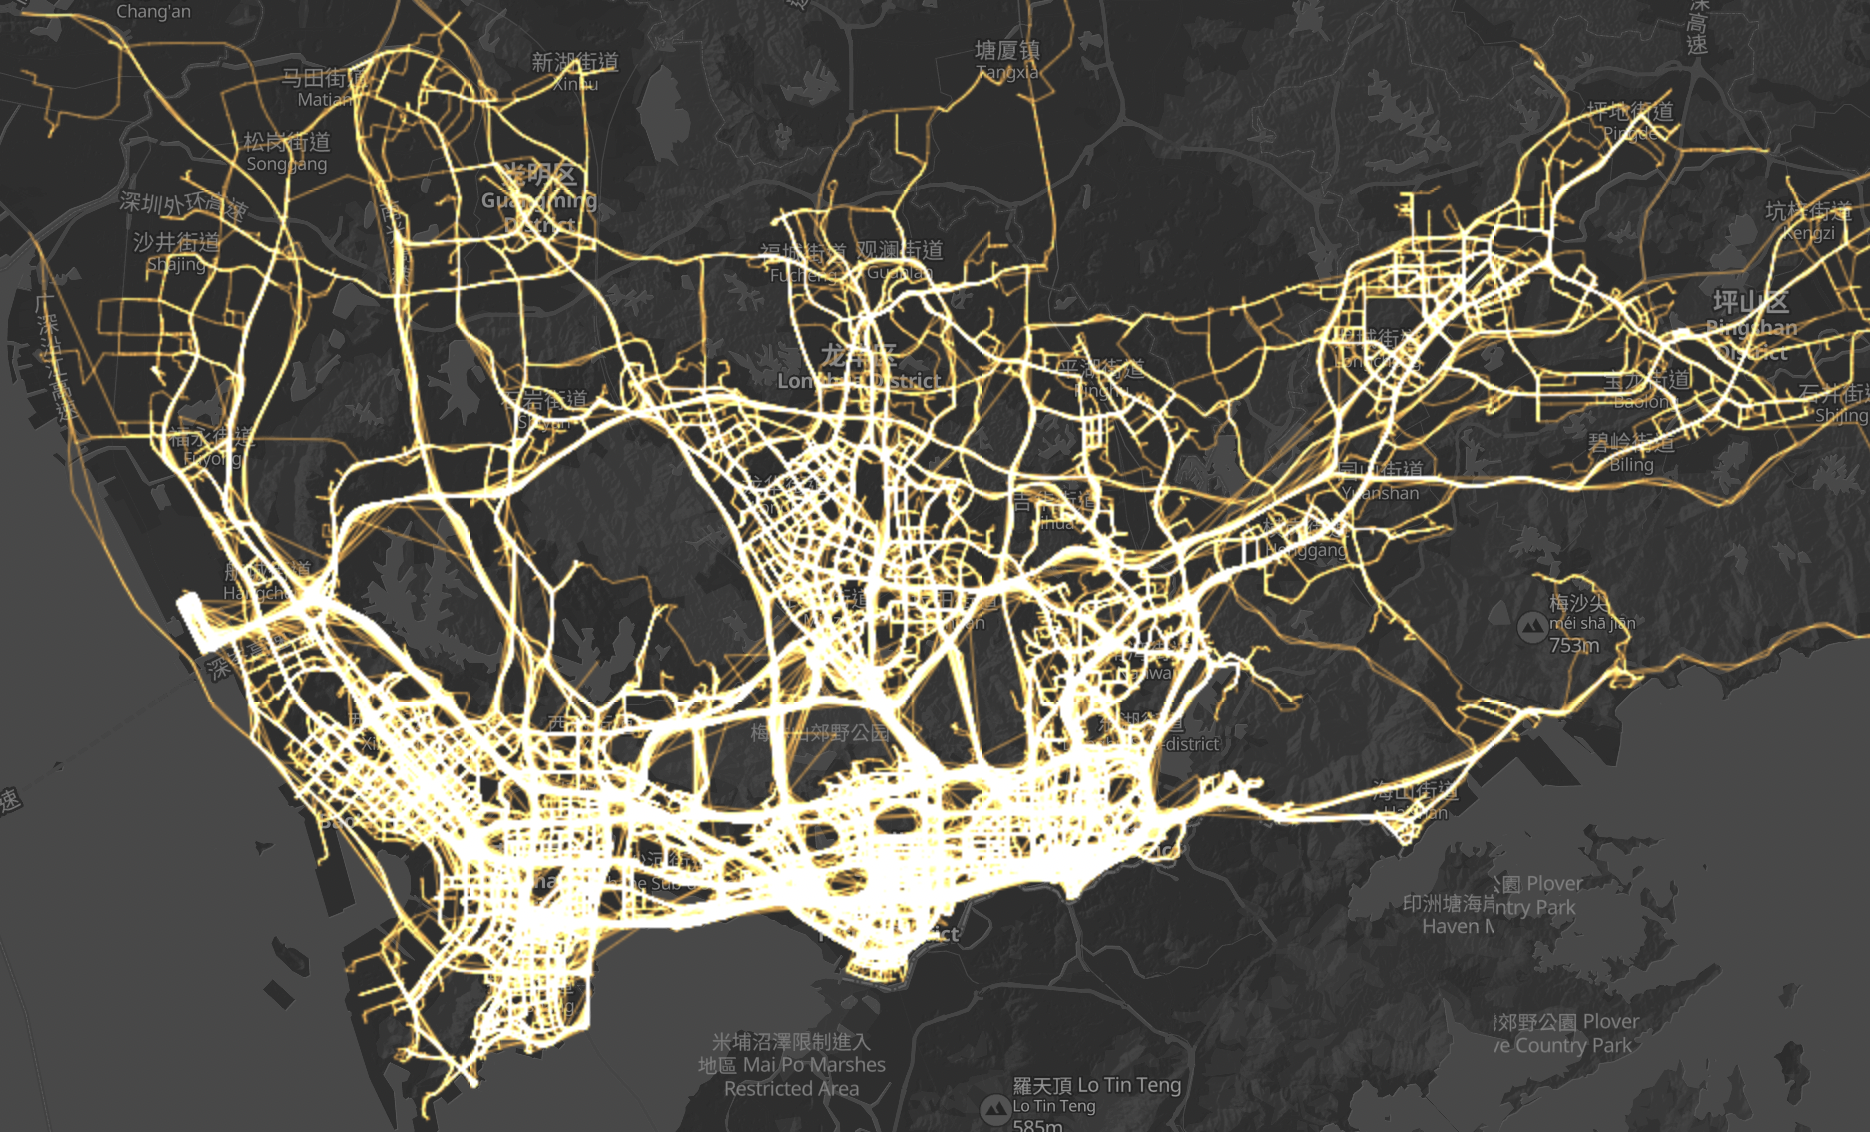
\includegraphics[width=\textwidth]{images/traj_map.png}
    \caption{Shenzhen taxi trajectories heatmap.}
    \label{fig: traj_map}
  \end{figure}

Based on these facts, we believe that the trajectories will give us the actual road transfer information. By analyzing road transfer, we propose a concept named \textit{trajectory-based road correlation} that stands for the relevance or similarity among roads. With this, a better spatial dependency can be captured. Therefore, the focus of this paper is to design a general method to extract road correlation through trajectories and utilize it for state-of-the-art neural networks to predict traffic state.

To summarize, in this paper, we propose a procedure to learn \textit{trajectory-based road correlation} via GPS data and use it to improve traffic state prediction.

The contribution of our paper is:
\begin{itemize}
    \item We build a road-network-based trajectory dataset upon completely raw GPS data.
    \item We propose a procedure to learn road correlation through trajectories.
    \item We improve traffic state prediction by utilizing the \textit{trajectory-based road correlation}.
\end{itemize}


\section{Related Work}
\textbf{Public Traffic Datasets.} There are several public traffic datasets which are frequently used for traffic prediction. They can be briefly categorized into three classes by spatial domain, which are \textbf{grid-based}, \textbf{sensor-based} and \textbf{road-network-based}.

For grid-based datasets, there are \textit{TaxiBJ}\cite{taxibj} that consists of the taxi in and out flow data in Beijing, and \textit{TaxiNYC} for taxis in New York City published by the New York City Taxi and Limousine Commission (TLC). For sensor-based datasets, \textit{METR-LA}\cite{DCRNN} and \textit{PEMS-BAY} are the most widely used datasets in urban traffic prediction area. In detail, \textit{PEMS-BAY} is collected from 325 sensors all over the San Jose bay area every 5 minutes. The traffic sensors can directly record the traffic flow of each road, which makes the dataset easy to handle and process. And for road-network-based datasets, \textit{Didi GAIA}'s open data has a good quality but they are seldom applied to build a model. It is GPS data containing taxi locations with timestamp that collected by \textit{Didi} company's mobile app, which is similar to ours. In conclusion, as suggested by Jiang and Luo\cite{surveyGNN}, most traffic prediction models are built upon traffic sensor datasets, while road-network-based datasets are mainly used for test. Therefore, we need to make better use of it.

\vspace{\baselineskip}

\textbf{Road Network Modeling.} Road network is the basic component of urban traffic system. To make use of the spatial information inside it, many approaches have been proposed. Statistical models are used to represent road network. For recent traffic prediction articles, Li et al.\cite{AAAI21} model road transition as a Markov Process over road network and use a first order Markov matrix to represent it. The growth of deep learning models makes it possible to model more complex road network and learn road characteristics efficiently. In basic GCN\cite{GCN0}, the authors use adjacency matrix to calculate Graph Laplacian Matrix in order to represent the whole graph. Lately, Wu et al.\cite{roadrep} proposed a hierarchical graph neural networks to capture both structural and functional characteristics of road network through several pre-defined attributes of each road. Wu et al.\cite{GWNET} use graph convolution to learn a new adjacency matrix of sensor graph, which is quite related to our work. To conclude, the two methods mentioned above need prior knowledge or history traffic state of roads. In contrast, our work is to learn a representation of each road to model its spatial characteristics only by trajectories.

\vspace{\baselineskip}

\textbf{Traffic Prediction Models.} Early attempts use traditional time series forecasting model including ARIMA\cite{ARIMA_pred} and VAR\cite{var_pred}, as well as machine learning techniques like k-NN\cite{knn_pred} and SVM\cite{svm_pred}. As mentioned in section 1, these models cannot capture the spatiotemporal dependency well. Many state-of-the-art deep neural networks have been proposed in the last several years. Yu et al.\cite{STGCN} proposed two different convolution blocks to capture spatial and temporal dependencies separately. Li et al.\cite{DCRNN} take advantage of seq2seq\cite{seq2seq} architecture and perform diffusion convolution on the graph. From our observation, few existing work leverage trajectories in traffic prediction. Hui et al.\cite{trajnet} extract the temporal features of roads by convolution with recent, daily-periodic and weekly-periodic traffic state data. Then they perform feature smoothing by propagating features through trajectories. On the contrary, our work attempts to combine the spatial representation that learned from trajectories into traffic state prediction models.


\section{Preliminaries}
In this section, we first give an overview of our whole work. And we will introduce the notations used in this paper and problem definitions in our task.

\subsection{Overview}
\begin{figure}[htb]
    \centering
    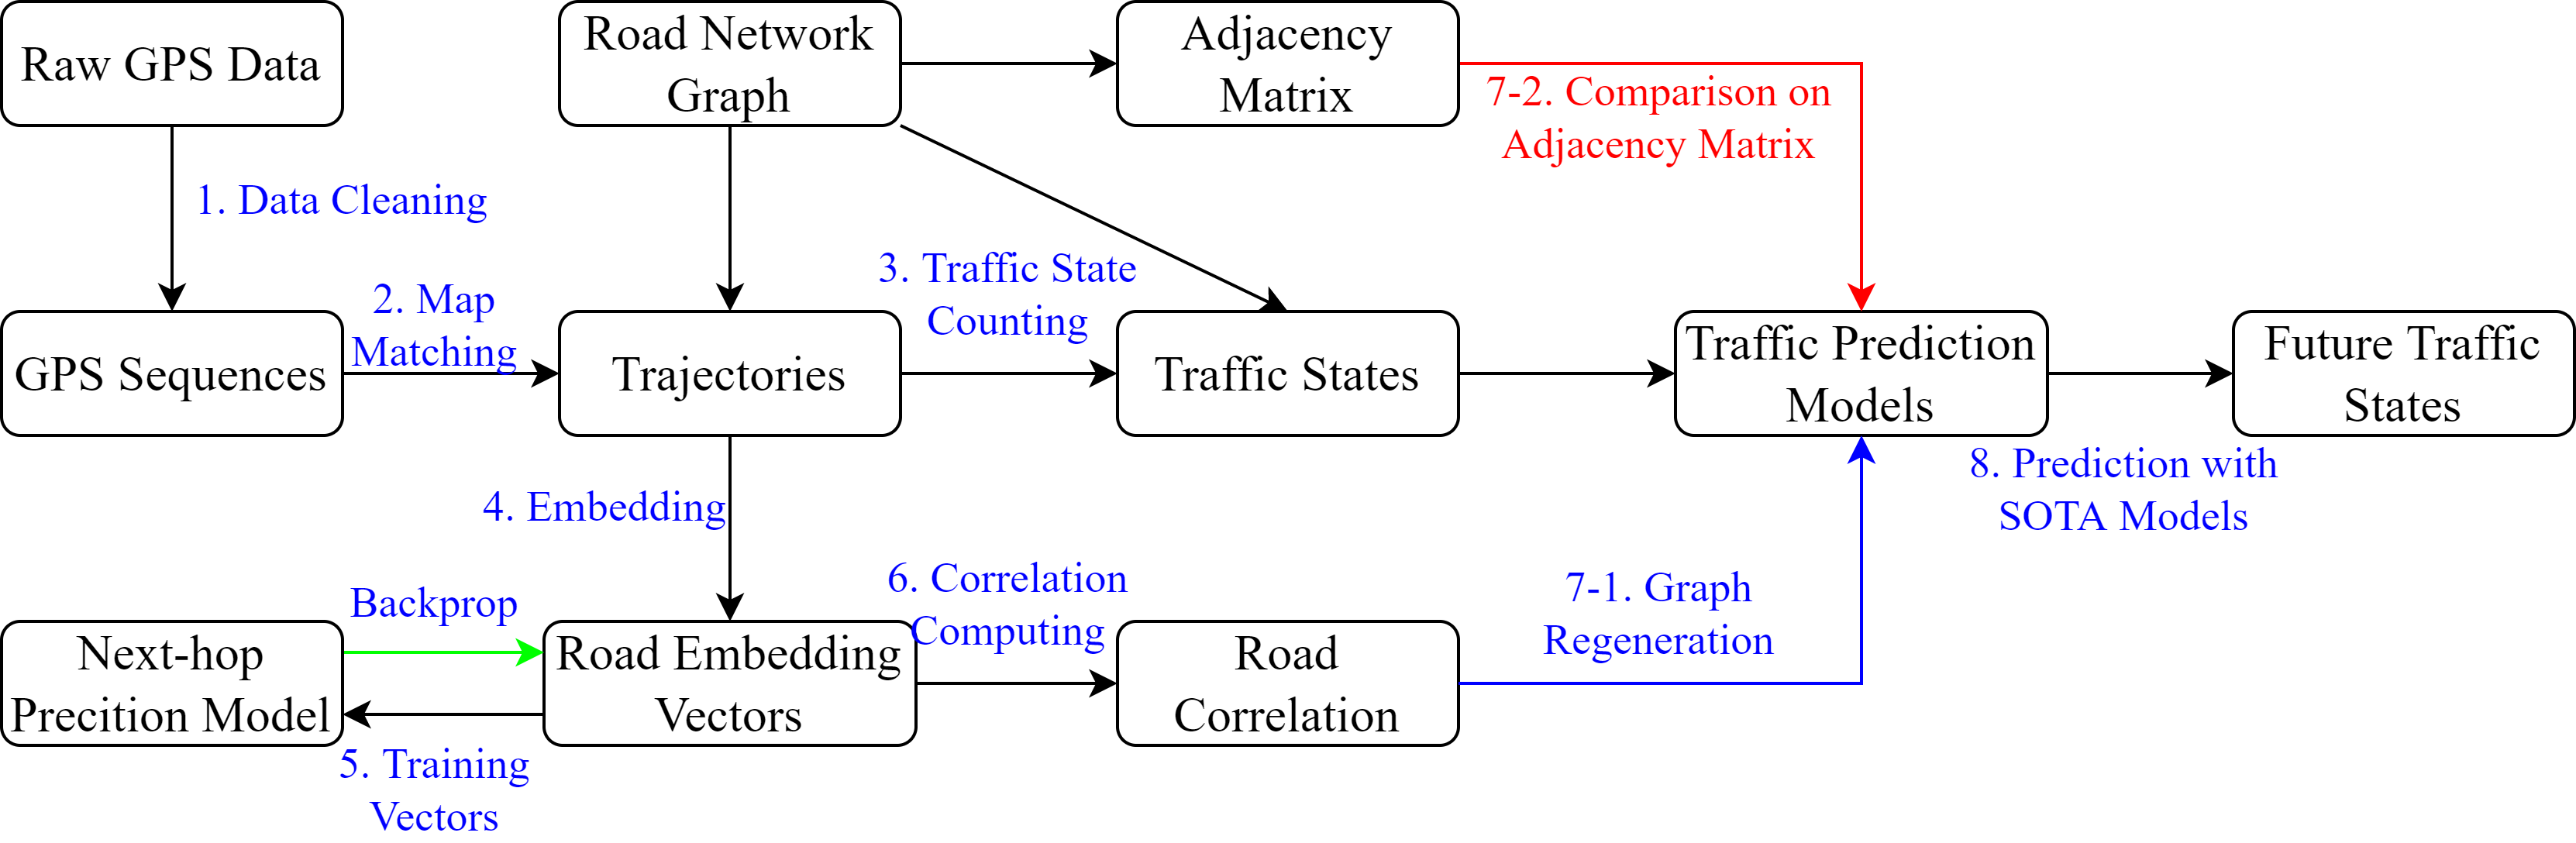
\includegraphics[width=\textwidth]{images/overview.drawio.png}
    \caption{An overview of our work.}
    \label{fig: overview}
\end{figure}

Figure \ref{fig: overview} provides an overview of this paper, and the details of each part will be stated in the following sections. Section 4 introduces how we build the dataset. The adopted methodology and model structure will be given in section 5. In section 6, the proposed model is verified by our dataset, and the experiment results demonstrate its practicability. A brief conclusion and several potential directions are provided in the last section.

\subsection{Notations}
Table \ref{notation_table} gives the notations and their definitions.
\begin{table}[h!]
    \begin{center}
        \caption{Notations}
        \label{notation_table}
        \begin{tabular}{cl}
            \toprule

            \textbf{Notation} & \textbf{Definition}                       \\

            \midrule

            $n_{(\cdot)}$     & number of some entities                   \\
            $d_{(\cdot)}$     & vector dimension                          \\
            $\mathcal R$      & road set                                  \\
            $r$               & a single road in $\mathcal R$             \\
            $\mathcal E$      & edge set                                  \\
            $A$               & adjacency matrix                          \\
            $\mathcal G$      & road network graph                        \\
            $\mathcal T$      & trajectory set                            \\
            $T$               & a trajectory in $\mathcal T$              \\
            $ts$              & timestamp                                 \\
            $s$               & speed                                     \\
            $w$               & window size                               \\
            $p$               & random sampling proportion                \\
            $E$               & road embedding matrix                     \\
            $\mathbf{e}_i$    & embedding vector for road $r_i$           \\
            $C$               & road correlation matrix                   \\
            $t$               & time interval                             \\
            $X$               & traffic state matrix                      \\
            $\mathbf x_t$     & traffic state vector at time interval $t$ \\

            \bottomrule
        \end{tabular}
    \end{center}
\end{table}

\subsection{Problem Definition}
This subsection gives the definitions\cite{AAAI21} of the concepts and tasks occur in this paper.
\begin{definition}[Road Network Graph]
    The road network can be represented by a directed graph $\mathcal{G}=(\mathcal{R}, \mathcal{E}, A)$, where $\mathcal{R}=\{r_1, r_2, \dots, r_{n_r}\}$ is a finite set of roads that each $r_i$ stands for a real road in the road network, which is an integer ID in practice. $\mathcal{E}$ is the set of directed edges where $(r_i, r_j)\in \mathcal{E}$ indicates that there is a directed edge from $r_i$ to $r_j$, i.e. $r_j$ is the downstream road in the road network. $A \in [0, 1]^{n_r\times n_r}$ is the adjacency matrix whose entry $A_{i, j}$ is a binary value that indicates whether there exists an edge $(r_i, r_j)\in\mathcal{E}$.
\end{definition}

\begin{definition}[Trajectory]
    Given a road network graph $\mathcal{G}=(\mathcal{R}, \mathcal{E}, A)$, a trajectory $T=[(r_1, s_1, ts_1), (r_2, s_2, ts_2), \dots, (r_l, s_l, ts_l)]$ is a sequence of (road, speed, timestamp) tuples. Each tuple $(r_i, s_i, ts_i)$ specifies that the vehicle is driving on $r_i$ with speed $s_i$ at timestamp $ts_i$. Besides, $\forall i=1, 2, \dots, l-1$, $r_i\neq r_{i+1}$ and $(r_i, r_{i+1})\in\mathcal{E}$.
\end{definition}

\begin{definition}[Traffic State]
    Traffic state stands for the traffic flow or speed of a road during a particular time interval. Traffic flow is defined as the number of vehicles passing by the road, and traffic speed is the average speed of these vehicles. For a road graph $\mathcal{G}=(\mathcal{R}, \mathcal{E}, A)$, we use $X\in\RR^{n_r\times n_t}$ to record the traffic state of each time interval. For time interval $t$, $\mathbf{x}_t=X_{:, t}\in\RR^{n_r}$ represents the traffic state of all roads during $t$.
\end{definition}

\begin{problem}[Next-hop Prediction]
    Given a road network graph $\mathcal{G}=(\mathcal{R}, \mathcal{E}, A)$ and the road sequence in a trajectory $T^r=\{r_1, r_2, \dots, r_l \}$ with length $l$, the trajectory next-hop prediction is to obtain a probability distribution $\hat P$ on road set $\mathcal{R}$ that best predicts the next step $r_{l+1}$. In conclusion, our goal is to build a model with parameters $\Theta$ that satisfies
    \begin{equation}
        \Theta=\mathop{\arg\min}_\Theta CrossEntropy(\hat P, P)
    \end{equation}
\end{problem}

\begin{problem}[Trajectory-based Road Correlation]
    Given a road network graph $\mathcal{G}=(\mathcal{R}, \mathcal{E}, A)$ and a trajectory set $\mathcal T$, find a road correlation function $Cor$ with respect to $\mathcal{T}$ which takes two roads as input and returns a real number $Cor(r_i, r_j)$ to quantify the spatial dependency between two roads $r_i$ and $r_j$. The value is bigger if the two roads have a stronger dependency, i.e. they frequently co-occur in same trajectories. The road correlation matrix $C\in\RR^{n_r\times n_r}$ stores all the correlation values s.t. $C_{i, j}=Cor(r_i, r_j)$.
\end{problem}

\begin{problem}[Traffic State Prediction]
    Given a road network graph $\mathcal{G}=(\mathcal{R}, \mathcal{E}, A)$, find a function $f$ and its parameter set $\Theta$ s.t. given historical traffic states $\{\mathbf{x}_{t-w_{in}+1}, \mathbf{x}_{t-w_{in}}, \dots, \mathbf{x}_t \}$ for an input window $w_{in}$, $f$ estimates the most likely traffic states $\{\mathbf{x}_{t+1}, \mathbf{x}_{t+2}, \dots, \mathbf{x}_{t+w_{out}} \}$ for an output window $w_{out}$.
    \begin{equation}
        \begin{aligned}
            \hat X_{:, t+1:t+w_{out}}&=f_\Theta(X_{:, t-w_{in}+1:t-1})\\&=\mathop{\arg\max}_{X_{:, t+1:t+w_{out}}} p(X_{:, t+1:t+w_{out}}|X_{:, t-w_{in}+1:t-1})
        \end{aligned}
    \end{equation}
\end{problem}


\section{Dataset}
This section introduces how we build the whole dataset from raw data.

TODO: 这里插一张总体流程图

\subsection{Data Description}
Our data is taken from the records of GPS devices on the taxis in Shenzhen. A brief description is as the following:
\begin{itemize}
    \item \textbf{Region:} Shenzhen
    \item \textbf{Time Range:} June 2020
    \item \textbf{Content:} Taxi GPS records
    \begin{itemize}
      \item License number
      \item Longitude and latitude
      \item Speed
      \item Timestamp
      \item $\cdots$
    \end{itemize}
  \item \textbf{Size:} Over 2,500,000,000 rows
\end{itemize}

A small part of data is shown as an example in figure \ref{fig: raw_data}.
\begin{figure}[htb]
    \centering
    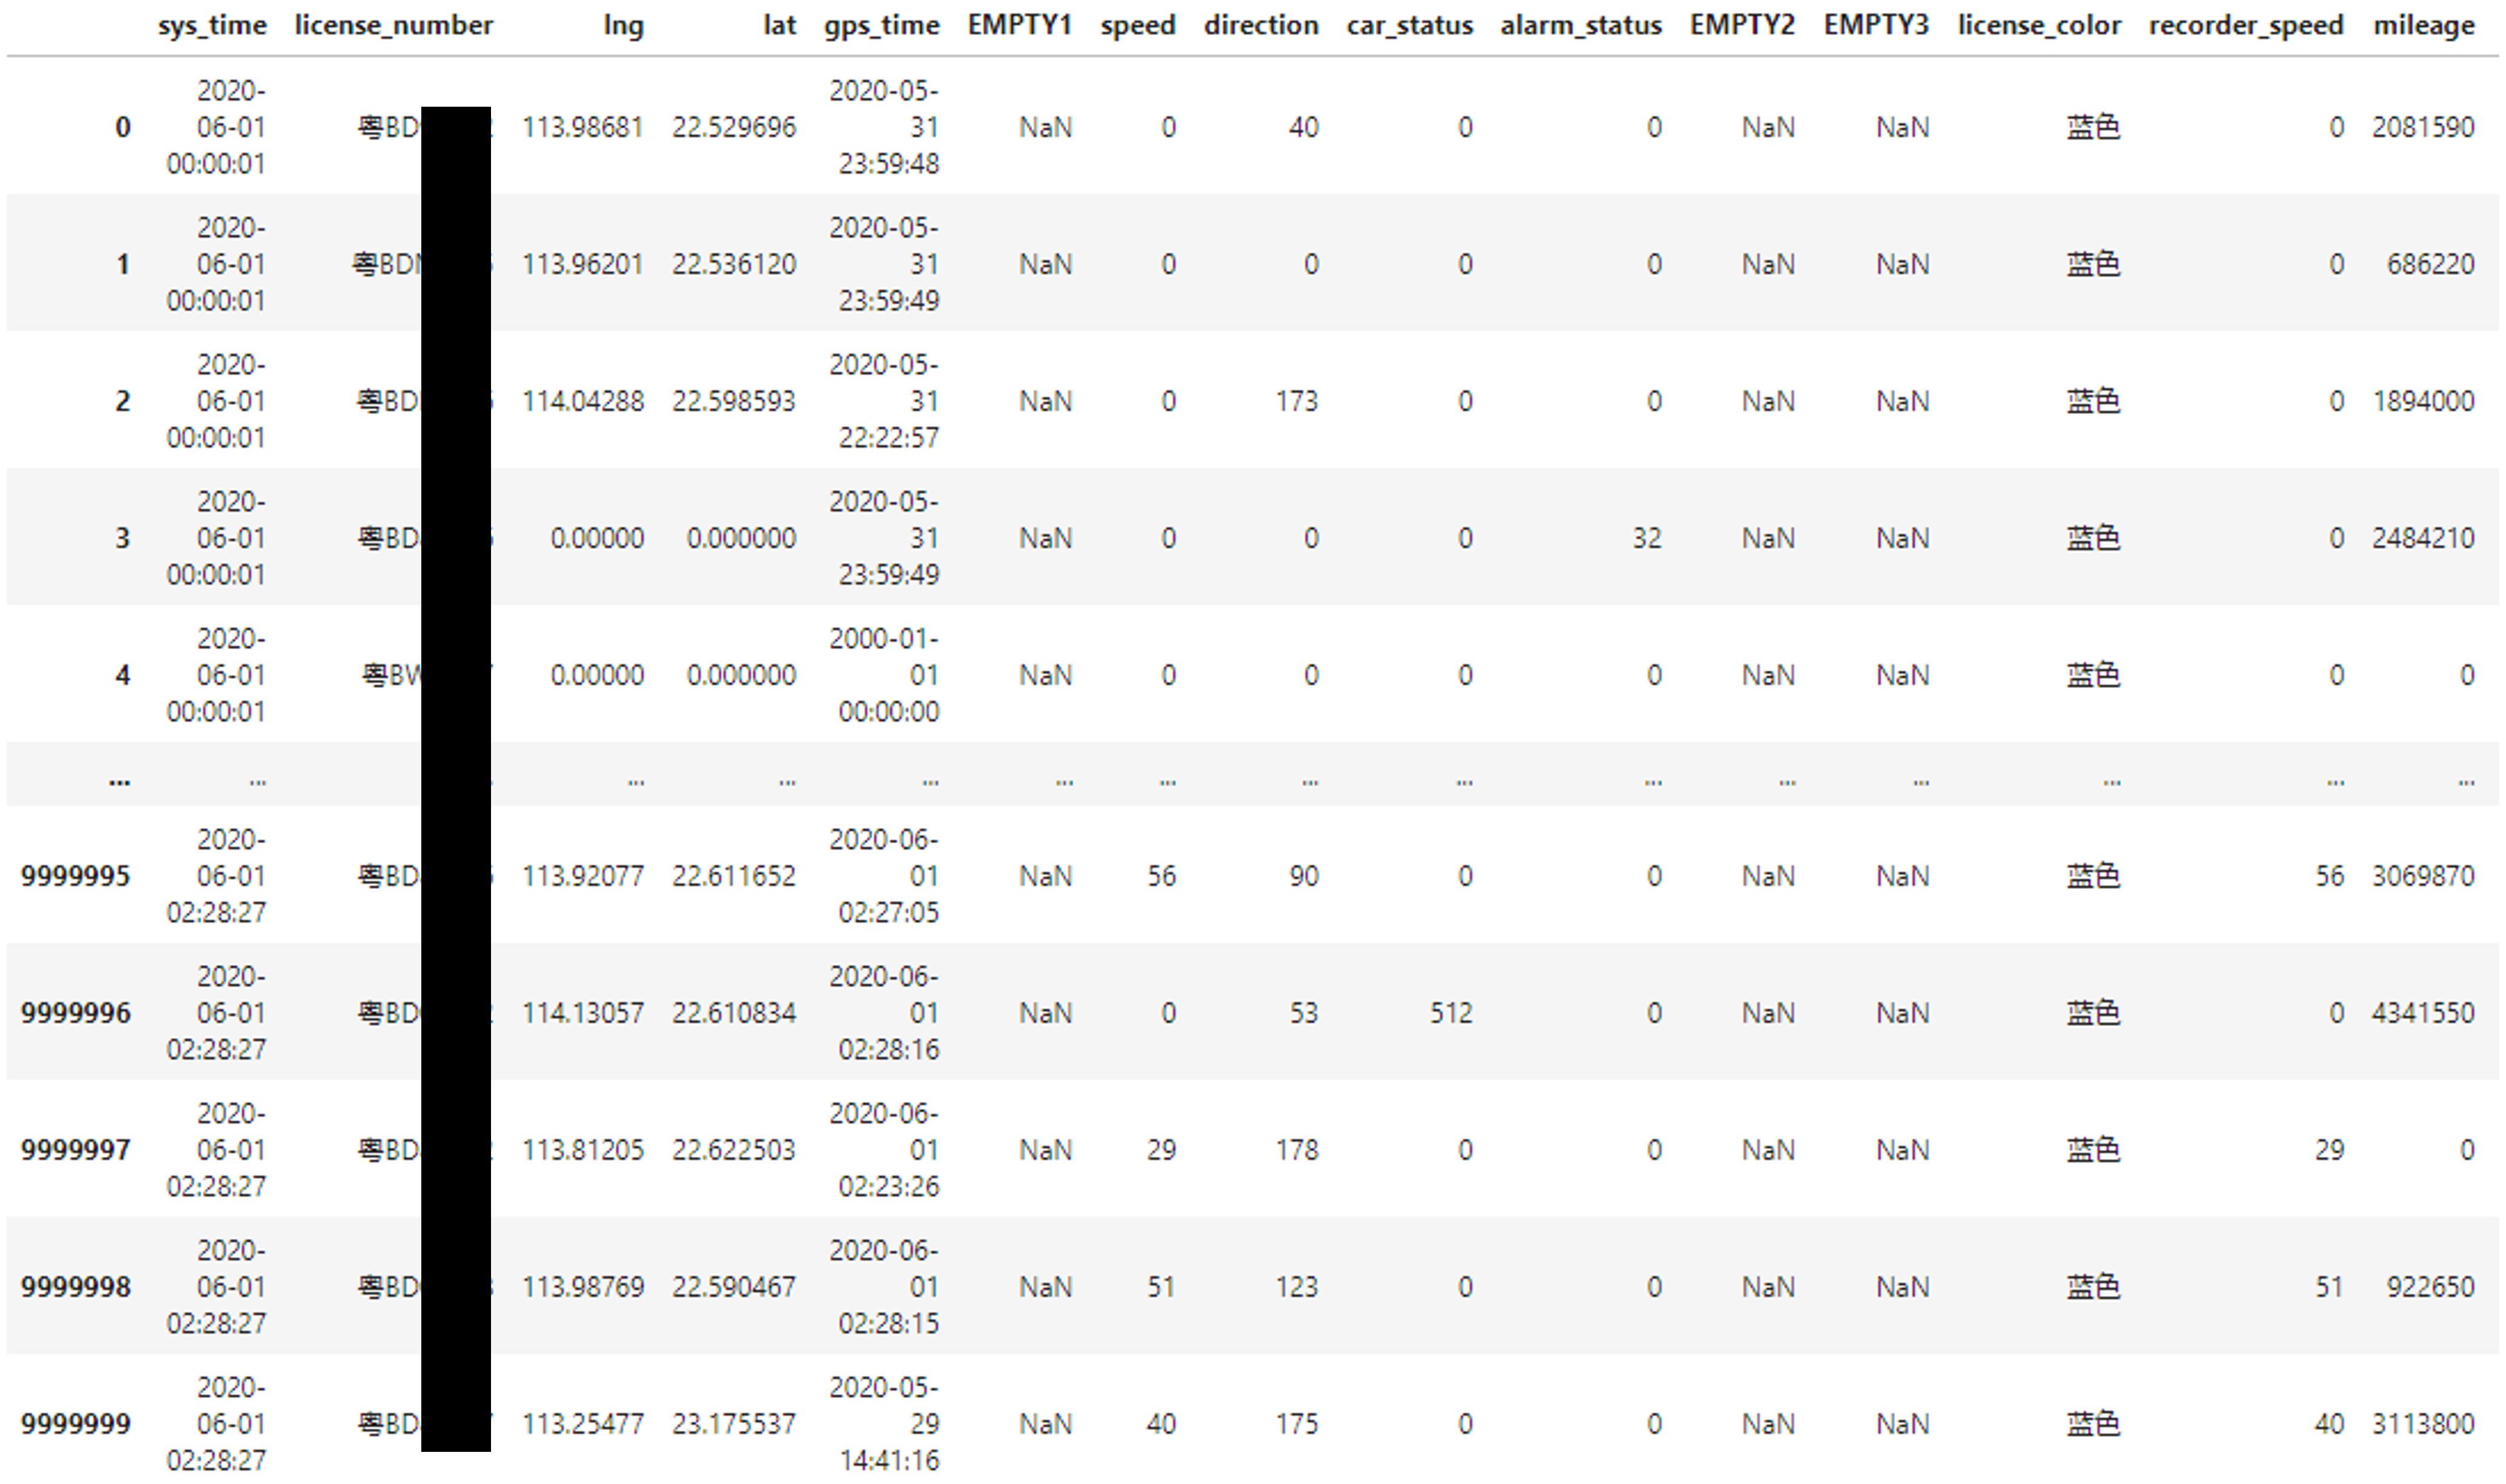
\includegraphics[width=\textwidth]{images/raw_data.png}
    \caption{A glance at Shenzhen taxi GPS raw data.}
    \label{fig: raw_data}
\end{figure}

Unlike the open datasets that can be applied to deep learning models without the need of data cleaning and completion, this raw dataset contains lots of abnormal values, which should be cleaned and re-organized carefully.

\subsection{Data Cleaning}
Data cleaning is the process of detecting and correcting (or removing) corrupt or inaccurate records from a record set, table, or database and refers to identifying incomplete, incorrect, inaccurate or irrelevant parts of the data and then replacing, modifying, or deleting the dirty or coarse data\cite{data_cleaning}. There are many kinds of bad records that should be deleted or modified. To summarize, we categorize them as the following classes.

\begin{enumerate}
  \item \textbf{Duplicate Rows.} A considerable large part of the raw data are duplicate. The reason is when a GPS device is transmitting data to server, it will send several copies in order to avoid packet loss under poor Internet connection. As a result, they are completely same rows, and thus can be removed safely, leaving only the foremost one.
  \item \textbf{Corrupted Timestamp.} This is a sort of abnormal record. Since our time range is June 2020, all the timestamps that not in here should be deleted. In detail, there are two kinds of them: 1) records in May $31^{st}$ or July $1^{st}$. This is caused by the equipments' lack of accuracy. 2) 2000-01-01. And this is caused by data loss, thus, it is filled by a default value.
  \item \textbf{Missing Location.} The latitude and longitude of some records are zero, which is resulted by the data loss during transmission. These dirty values should be deleted.
  \item \textbf{Zero Speed.} Stationary taxis are still transmitting their location information to the server if the GPS device is on, leading to a big portion of zero speed records. They are useless owing to that trajectories are a series of moving locations. Therefore, under normal circumstances, it is better to remove them. However, things are not that happy in our data. There are four kinds of zero speed records relating to the change of location, i.e. latitude and longitude, and they should be treated differently. Details are provided in the next subsection.
  \item \textbf{Irrelevant Attributes.} As shown in figure \ref{fig: raw_data} above, the raw data consists of several columns. The information that have no contribution to trajectories needs to be removed, leaving only latitude, longitude, speed and timestamp.
\end{enumerate}

We take the data of June $1^{st}$ as a case study to give an illustration of our data cleaning procedure and hope to reflect the property of the whole GPS data. In total, there are 97,453,725 rows. Table \ref{data_cleaning_table} gives the deleted percentage and remaining rows after each data cleaning step.

\begin{table}[htb]
  \begin{center}
      \caption{Data cleaning example on June $1^{st}$.}
      \label{data_cleaning_table}
      \begin{tabular}{ccc}
          \toprule

          \textbf{Step} & \textbf{Deleted Percentage} & \textbf{\#Remaining Rows}\\

          \midrule

          Drop duplicate & $51.73\%$ & 47,042,104\\
          Drop abnormal values & $1.19\%$ & 45,874,548\\
          Drop zero speed & $16.84\%$ & 29,458,603\\

          \cmidrule{1-2}

          \textbf{Remaining Percentage} & $30.22\%$ & ~\\

          \bottomrule
      \end{tabular}
  \end{center}
\end{table}

As shown in the table, half of the records are duplicated. Fortunately the total number of records are large enough to endure the data cleaning procedure. For the $17\%$ zero speed records, the following figure \ref{fig: speed_distribution} points out the huge impact of its removal on the distribution of speed.

\begin{figure}[htb]
  \centering
  \caption{Speed distribution before and after cleaning.}
  \label{fig: speed_distribution}
  \begin{subfigure}[t]{0.45\linewidth}
      \centering
      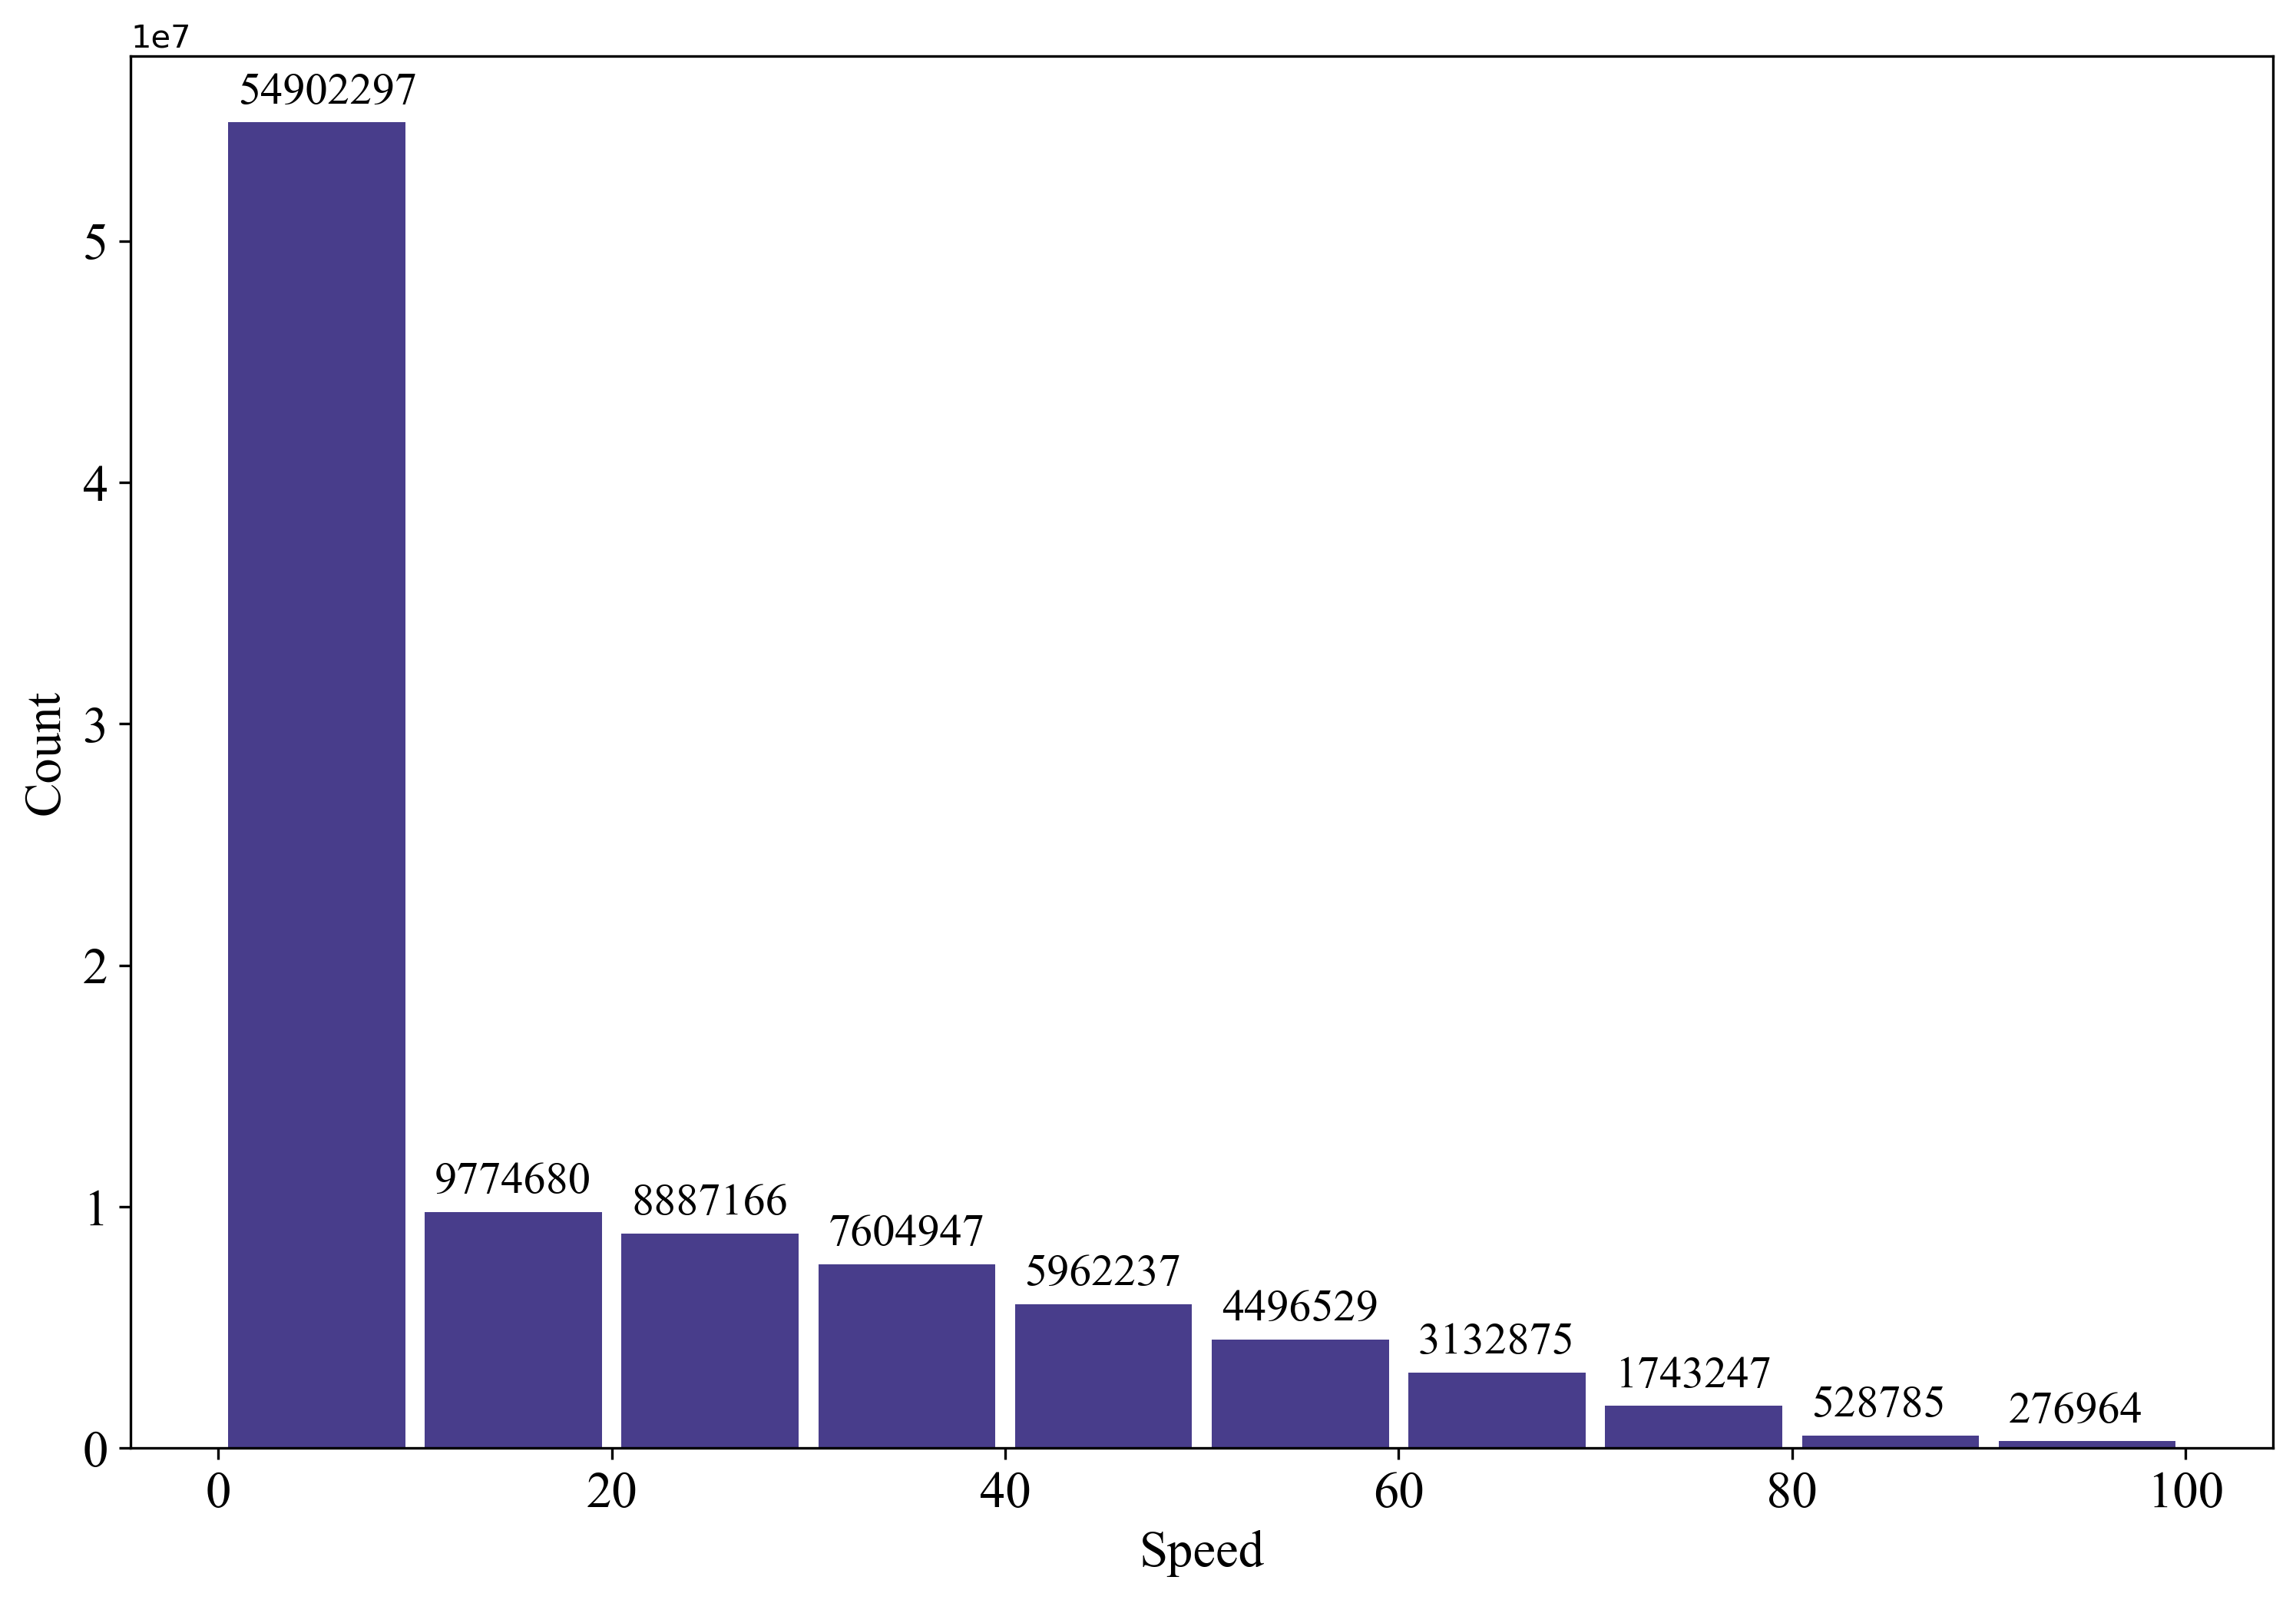
\includegraphics[width=\textwidth]{images/speed_hist_before.png}
      \caption{Before}
      \label{fig: speed_before}
  \end{subfigure}
  \begin{subfigure}[t]{0.45\linewidth}
      \centering
      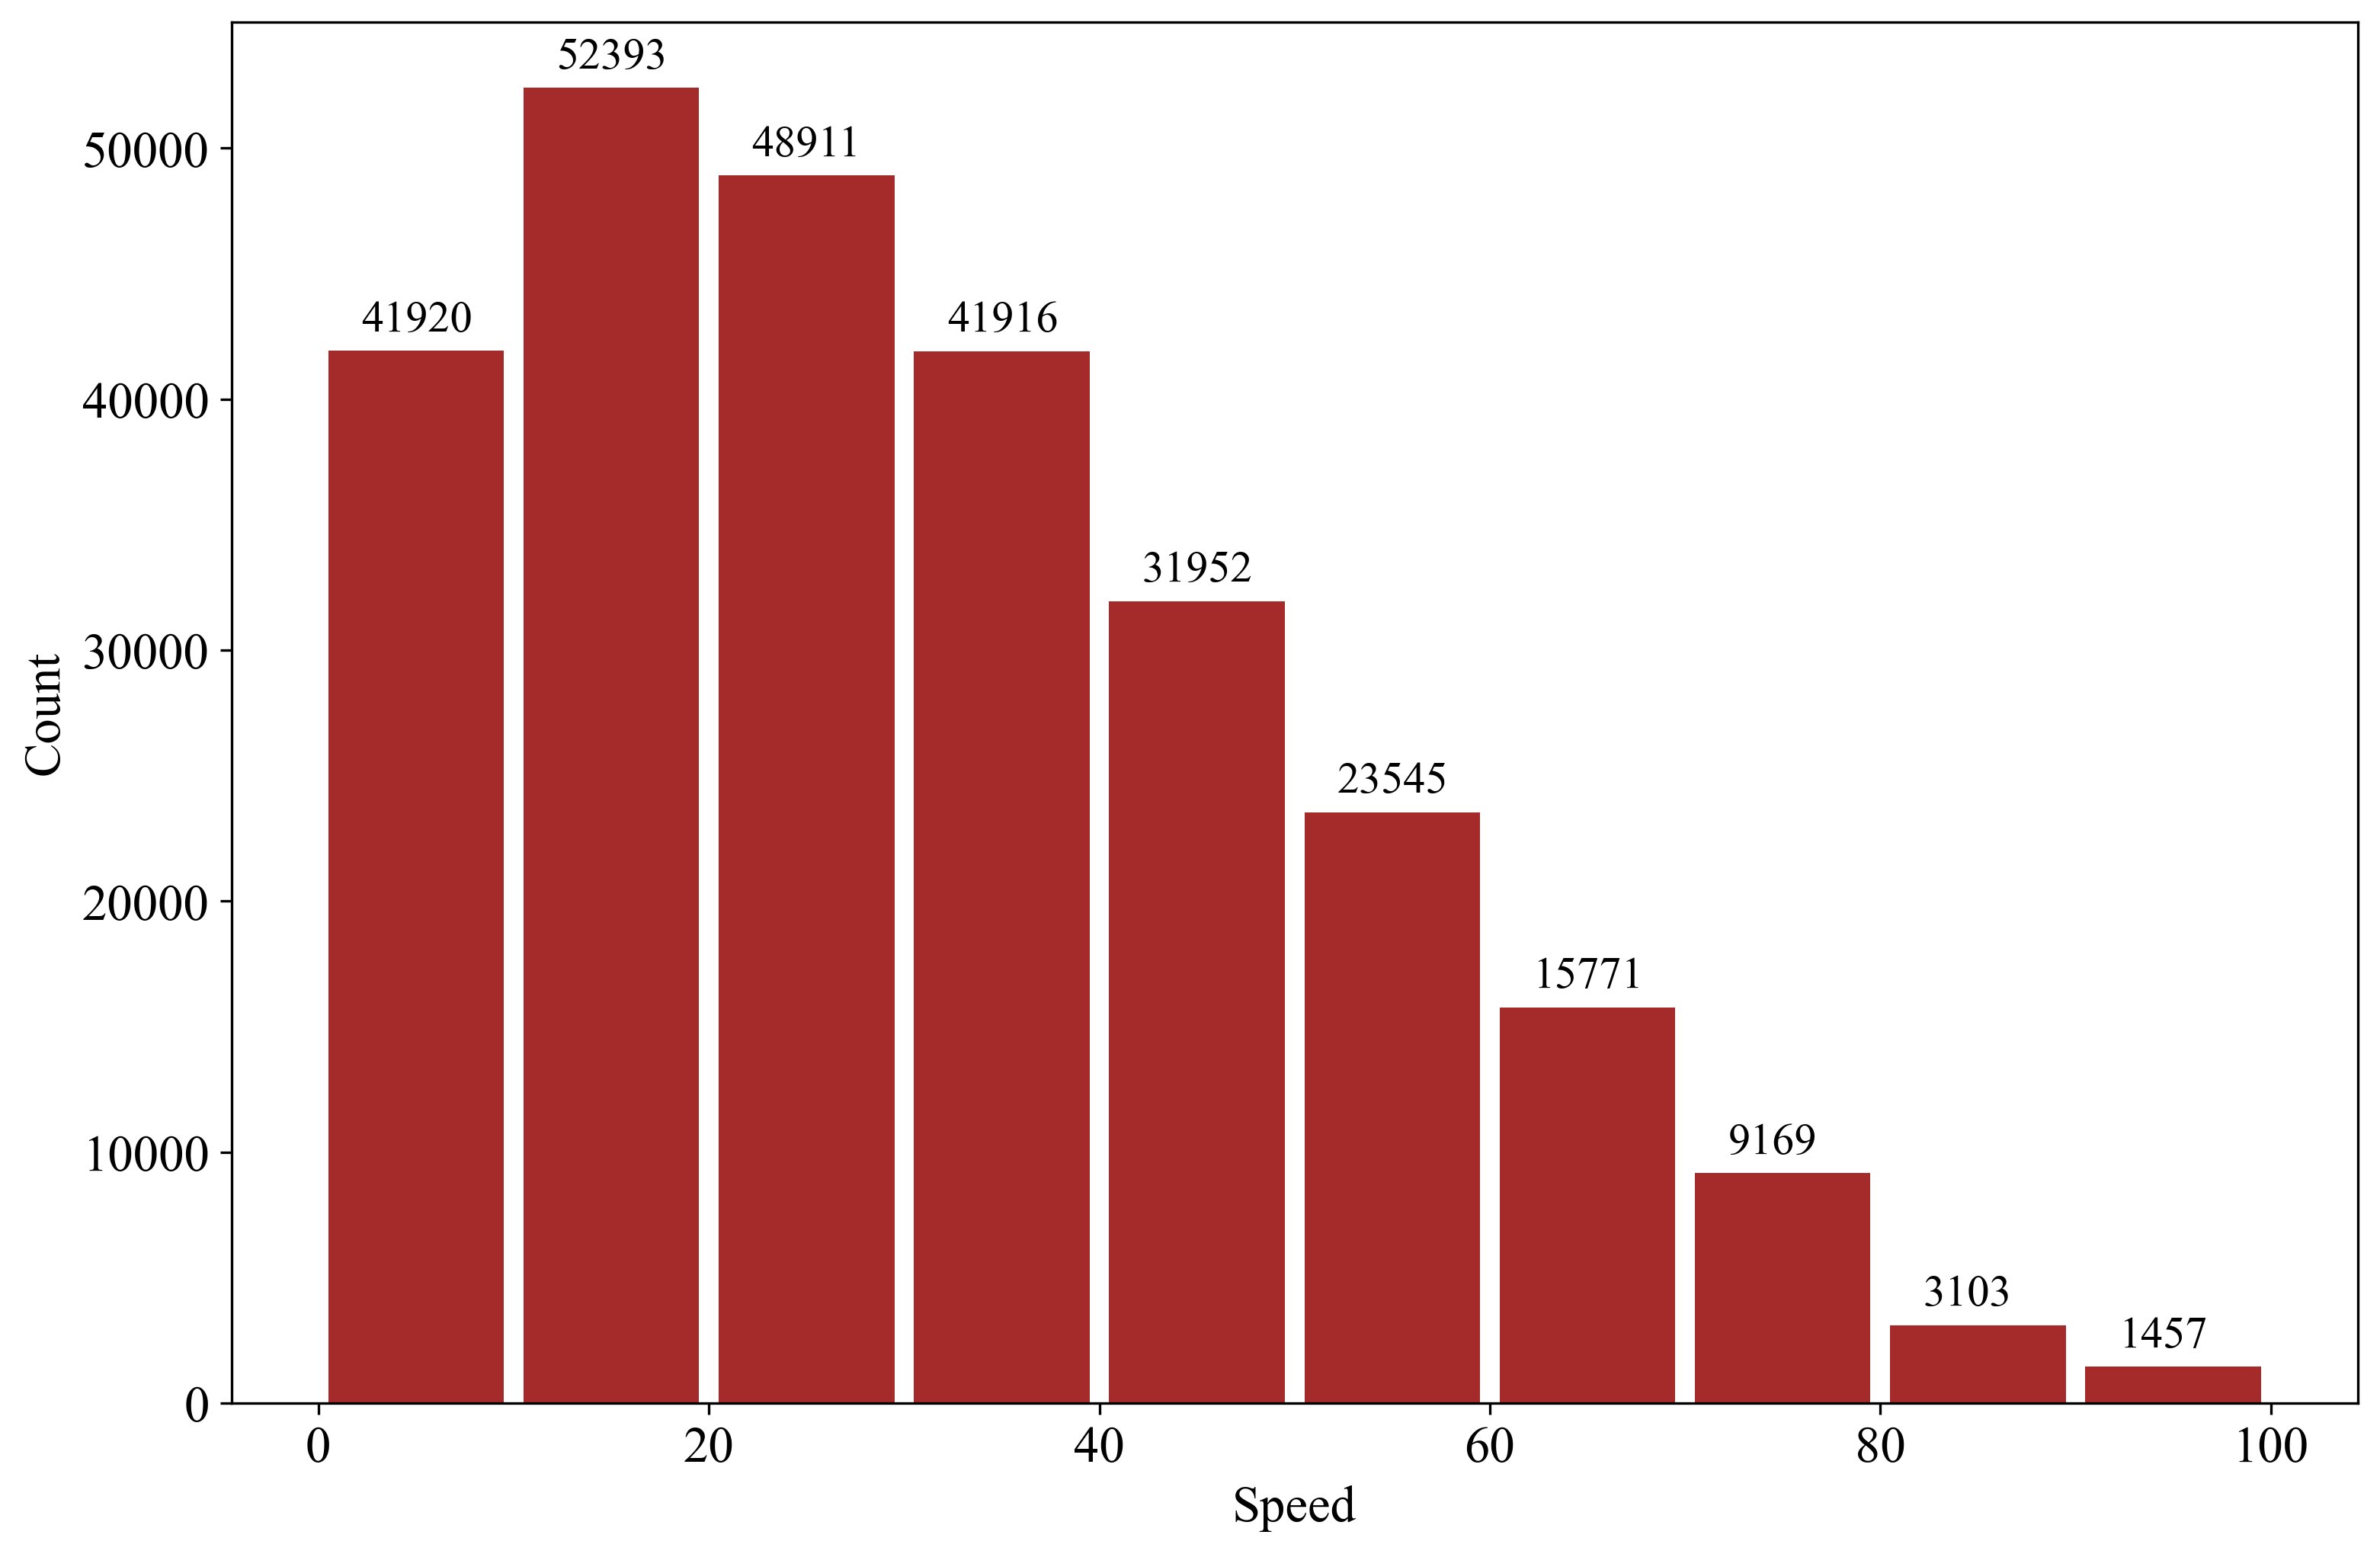
\includegraphics[width=\textwidth]{images/speed_hist_after.png}
      \caption{After}
      \label{fig: speed_after}
  \end{subfigure}
\end{figure}

After data cleaning, we get the GPS point sequences of each car, the next step is to match them to the road network according to their location. But first, we need to draw the GPS points on the map and check if there is any shift with roads, which is related to the coordinate system.

\begin{figure}[htb]
  \centering
  \includegraphics[width=\textwidth]{images/gps_seq.png}
  \caption{Visualization of cleaned GPS points.}
  \label{fig: gps_seq}
\end{figure}

Figure \ref{fig: gps_seq} shows that the GPS points are accurately moving along roads. The coordinate system we use is WGS84 (EPSG: 4326), which is the default for GPS service. Lots of Chinese GPS data is under GCJ-02, an encrypted version of WGS84. The location conversion between them is a complicated task, fortunately there is no need in our dataset.

\subsection{Road Network}
As mentioned in section 2, there are mainly three types of spatial graph that categorized by its vertices, which is grid, sensor or road. For a road network graph, a vertex represents a road and an edge stands for the connectivity between two roads. The formal definition has been given in section 3.2. In short, we need to acquire real road map and construct the graph depending on it.

\textit{OpenStreetMap (OSM)}\cite{osm} is a collaborative project to create a free editable geographic database of the world. It is easy to download a map and create a road network graph by \textit{OSM}'s official website\footnote{\href{https://www.openstreetmap.org/}{https://www.openstreetmap.org/}} and its Python API. Our data covers the taxi tracks over the whole Shenzhen, but it is impractical to construct the complete road network of the city due to its huge complexity. As a result, we decide to choose a small part of central business district (CBD) in Futian. The red rectangle in figure \ref{fig: gps_seq} encloses the roads we choose, and this is because \textit{OSM} can only export a rectangular region. Figure \ref{fig: roadmap} provides a closer look of these roads.

\begin{figure}[htb]
  \centering
  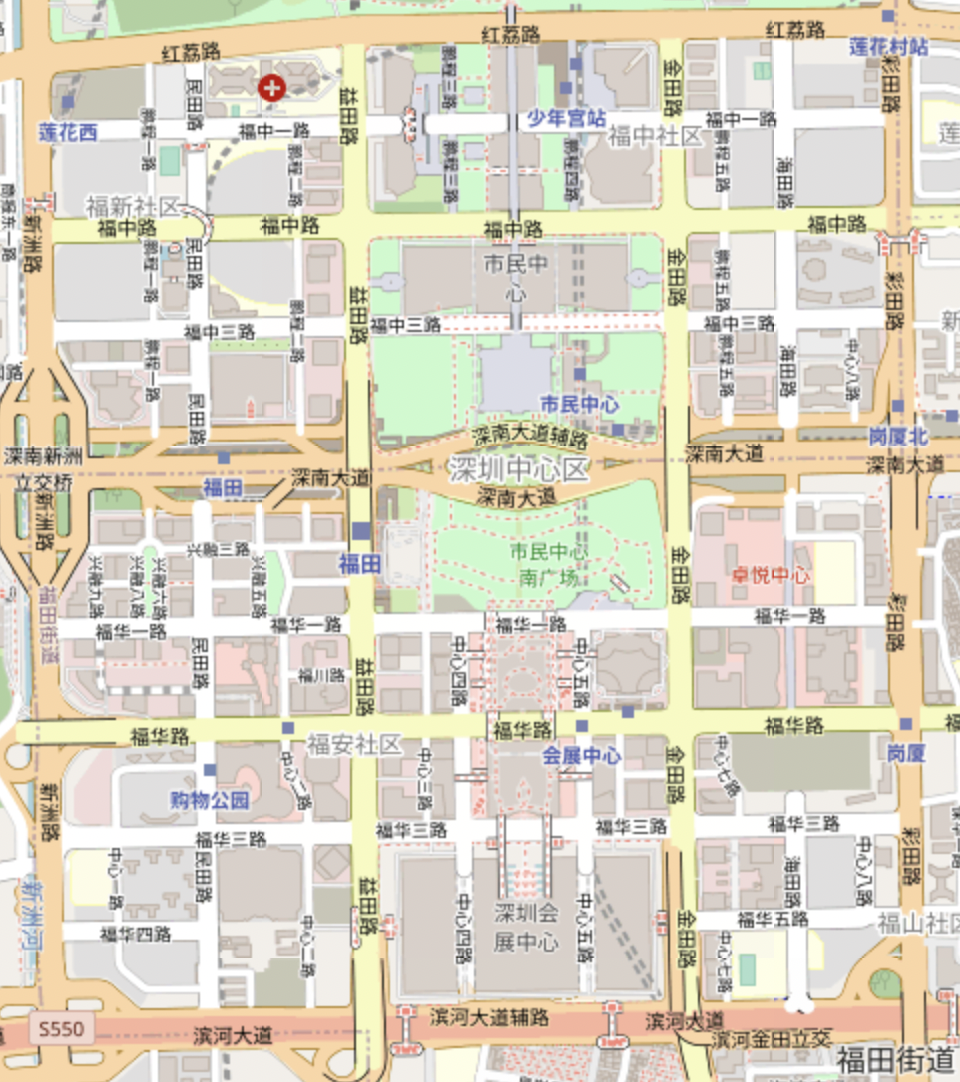
\includegraphics[width=\textwidth]{images/roadmap.png}
  \caption{The road map for graph construction.}
  \label{fig: roadmap}
\end{figure}

Having the boundary latitudes and longitudes, we can download the road network as a graph structure via Python. Figure \ref{fig: graph_before} offers the visualization of it. In short, the graph has 906 roads, 532 intersections and endpoints. However, this graph still contains plentiful tiny and redundant roads. This is mainly caused by the intersections\cite{grah_simplify}. To be specific, a road will be cut as two roads whenever there is an intersection on it, especially for crossroads. A crossroad is represented by 12 intersection points in the graph, leading to numerous tiny roads that can be merged into main roads. There are also many other cases that needs simplification. We summarize them as the following.

\begin{figure}[htb]
  \centering
  \caption{Road network graph before and after simplification.}
  \label{fig: graph}
  \begin{subfigure}[t]{0.45\linewidth}
      \centering
      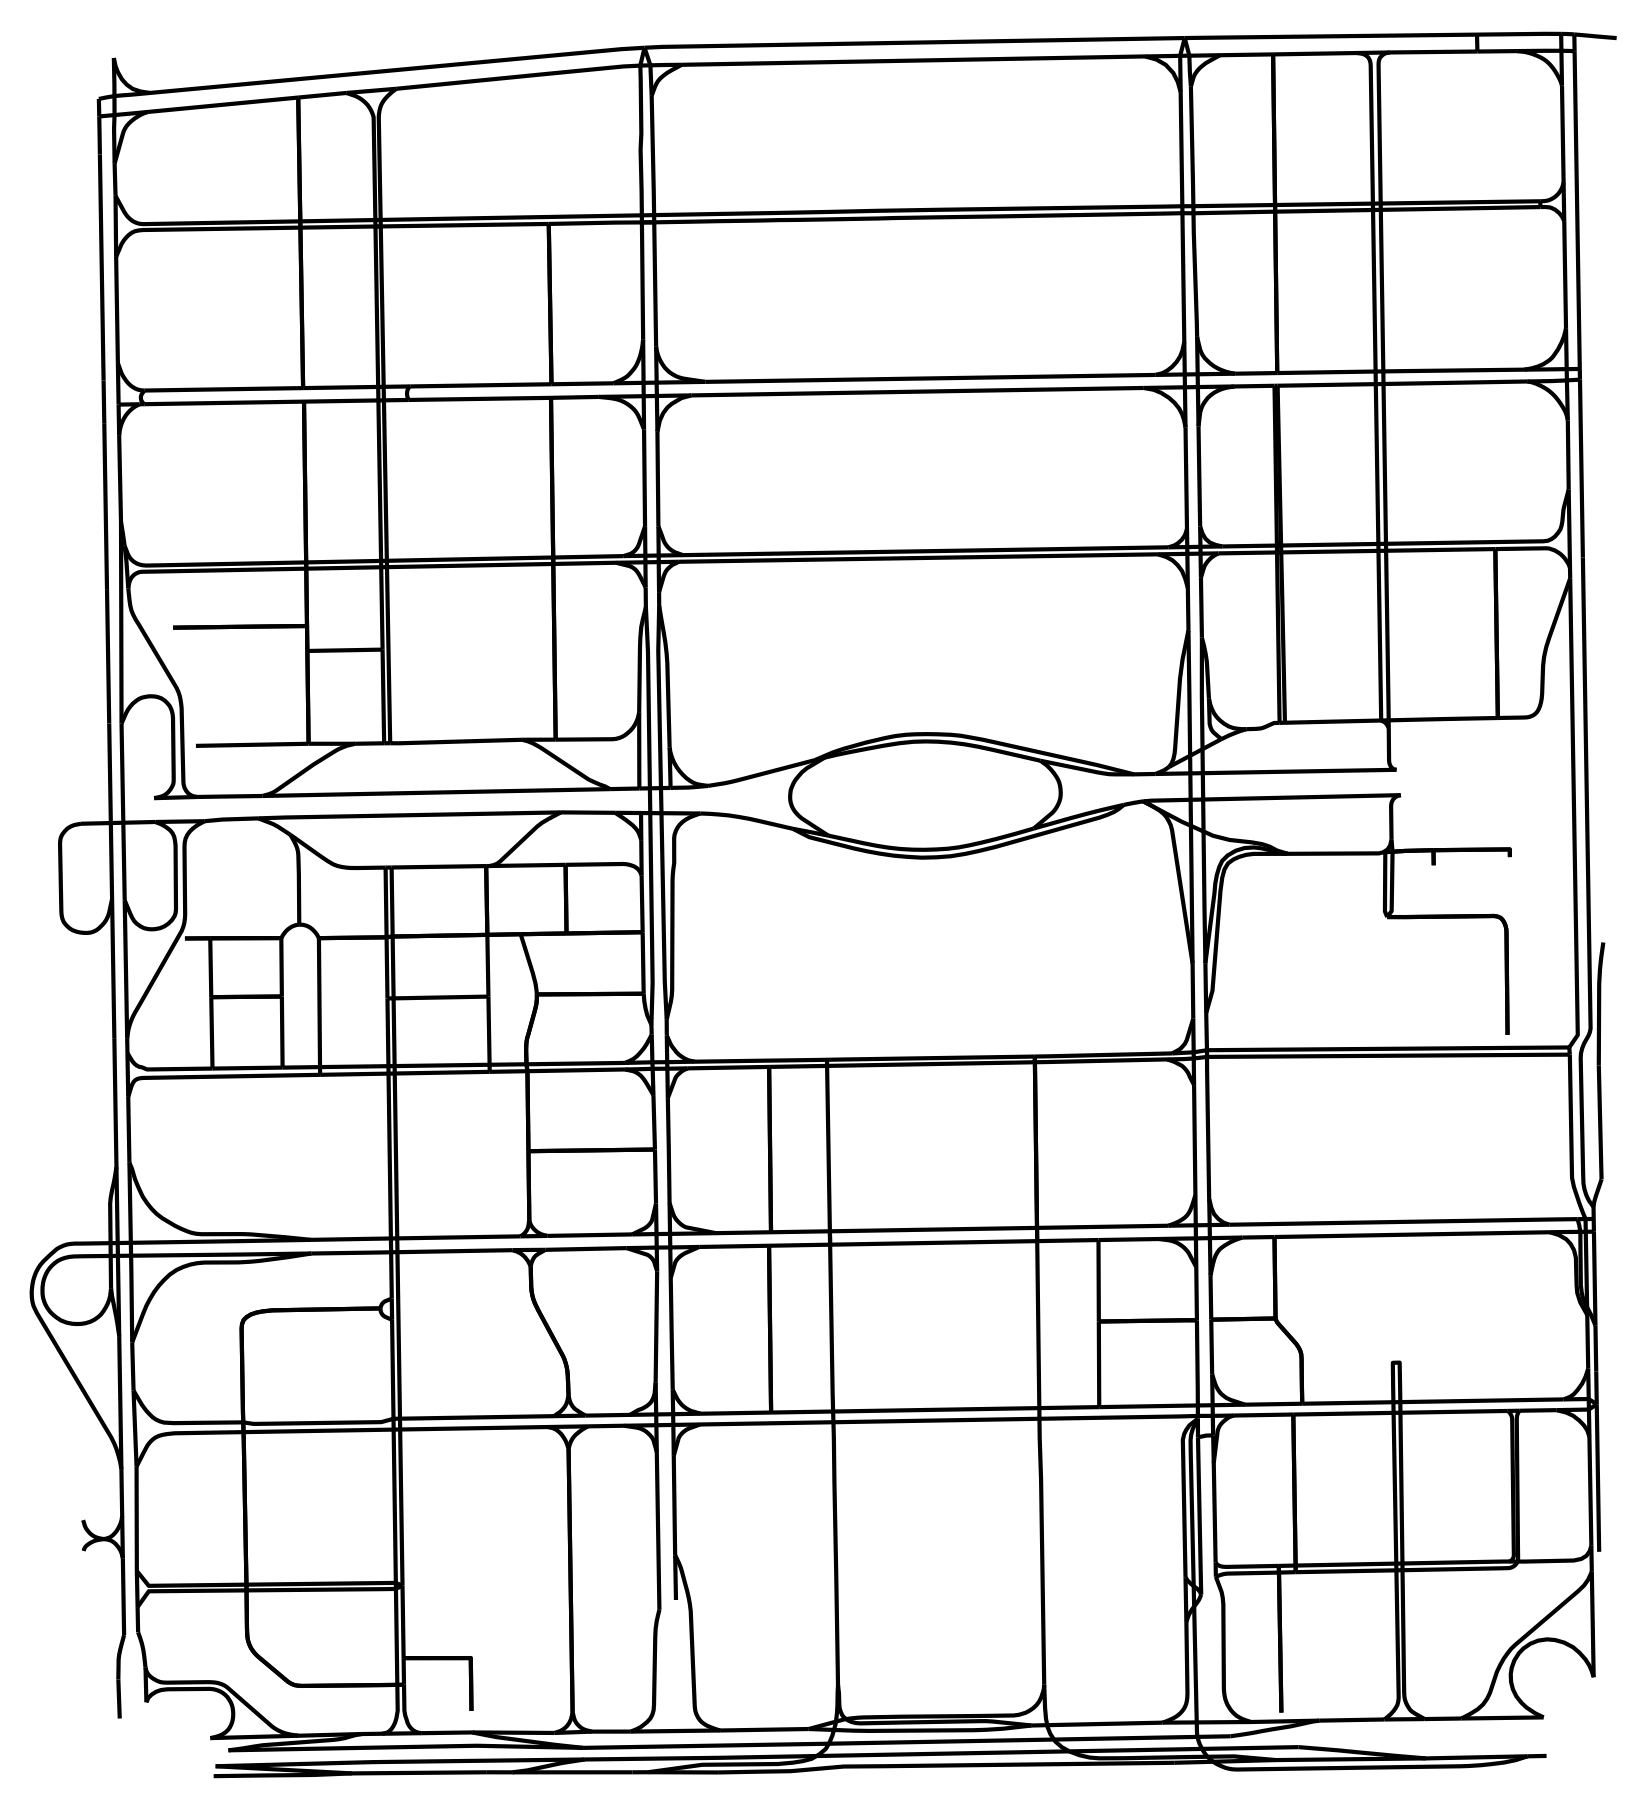
\includegraphics[width=\textwidth]{images/graph_before.png}
      \caption{Before}
      \label{fig: graph_before}
  \end{subfigure}
  \begin{subfigure}[t]{0.45\linewidth}
      \centering
      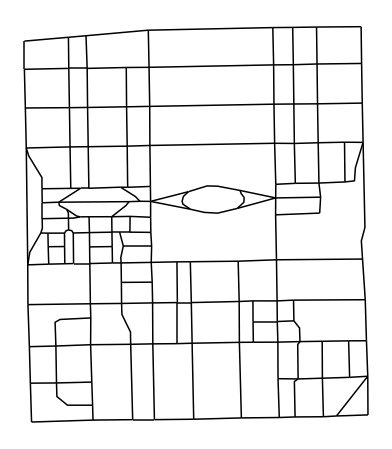
\includegraphics[width=\textwidth]{images/graph_after.png}
      \caption{After}
      \label{fig: graph_after}
  \end{subfigure}
\end{figure}

\begin{enumerate}
  \item \textbf{Redundant Roads Between Neighboring Intersections.} We have illustrated the reason in the paragraph above. To eliminate them, the simplest way is to merge the intersection points at crossroads.
  \item \textbf{Trailing Roads.} There are some roads not connected to the main road network at both ends. We decide to remove them since they take little effect in traffic.
  \item \textbf{Overpasses.} Overpass is a 3D structure that cannot be reflected in a 2D map. Therefore, the GPS points on overpasses are in a mess when plotting to map, and impossible to be matched on roads. They should be deleted and leaving only the underlying main roads.
  \item \textbf{Two-way Lanes.} Roads are bidirectional, which is faithfully reflected in the graph. However, it will cause a problem that the two lanes of a road do not share the same endpoints. For convenience, we combine them, and manually reverse the road for its bi-directionality.
\end{enumerate}

A visualization of these four cases is provided by figure \ref{fig: simplification}. To handle them, we use \textit{QGIS}\footnote{\href{https://qgis.org/en/site/}{https://qgis.org/en/site/}} as a tool to redraw the graph by ourselves. \textit{QGIS} functions as geographic information system (GIS) software, allowing users to analyze and edit spatial information, in addition to composing and exporting graphical maps. Figure \ref{fig: graph_after} shows the road network graph after simplification where the four cases are eliminated thoroughly.

\begin{figure}[htb]
  \centering
  \caption{Four simplification cases.}
  \label{fig: simplification}
  \begin{subfigure}[t]{0.22\linewidth}
      \centering
      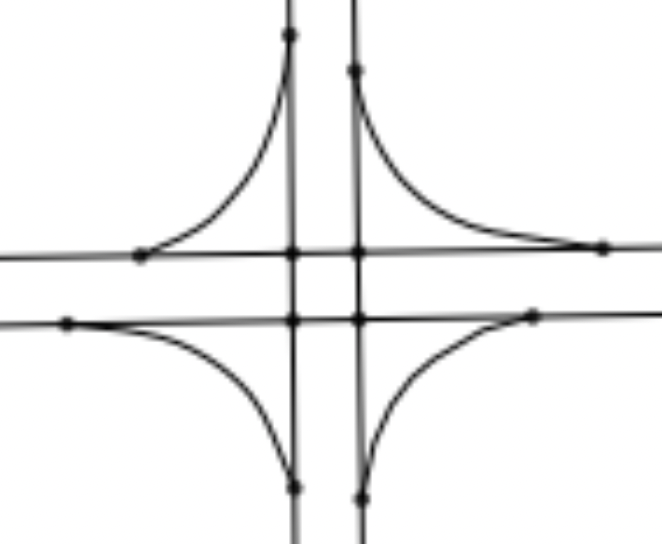
\includegraphics[width=\textwidth]{images/crossroad.png}
      \caption{Redundant Roads}
      \label{fig: redundant_roads}
  \end{subfigure}
  \begin{subfigure}[t]{0.22\linewidth}
      \centering
      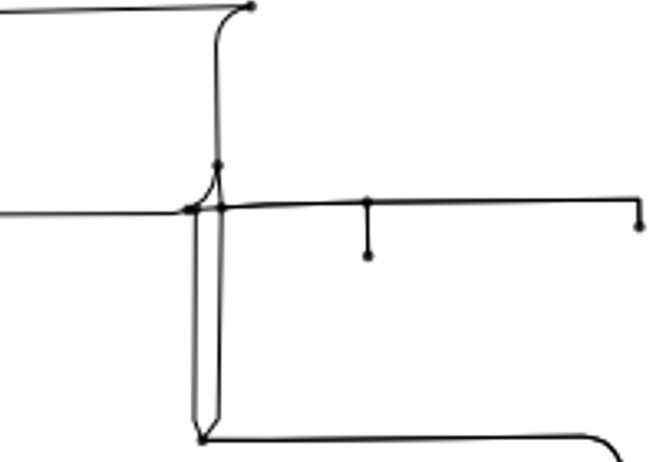
\includegraphics[width=\textwidth]{images/trailing_road.png}
      \caption{Trailing Roads}
      \label{fig: trailing_road}
  \end{subfigure}
  \begin{subfigure}[t]{0.22\linewidth}
    \centering
    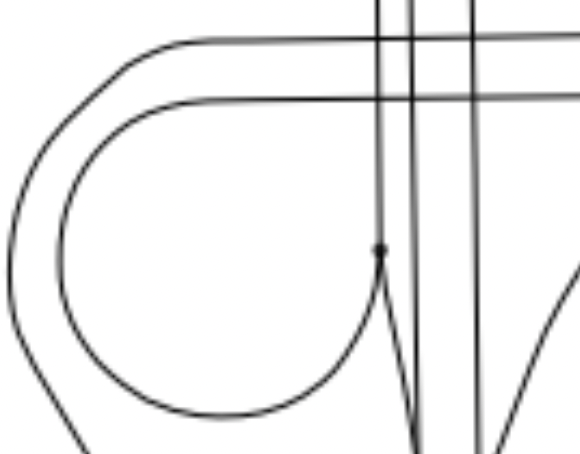
\includegraphics[width=\textwidth]{images/overpass.png}
    \caption{Overpass}
    \label{fig: overpass}
  \end{subfigure}
  \begin{subfigure}[t]{0.22\linewidth}
    \centering
    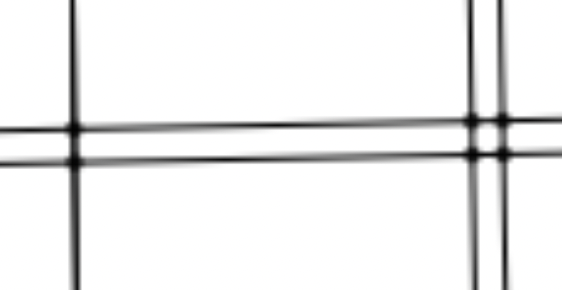
\includegraphics[width=\textwidth]{images/two-way.png}
    \caption{Two-way Lanes}
    \label{fig: two-way}
  \end{subfigure}
\end{figure}

\subsection{Map Matching}
Map matching\cite{mm} is a procedure to match a location, in this paper, a (latitude, longitude) pair, on a specific road to determine where the vehicle is travelling on. A variety of map matching algorithms have been proposed by researchers around the world in recent years, such as Hidden Markov Map Matching\cite{HMMM}, ST-Matching\cite{stmm} and Fast Map Matching\cite{fmm}. We tried several map matching functions and eventually choose Fast Map Matching (FMM) because of its fastest speed and open-source library.

\begin{table}[htb]
  \begin{center}
      \caption{\textit{FMM} tuned parameters.}
      \label{fmm_table}
      \begin{tabular}{cll}
          \toprule

          \textbf{Parameter} & \textbf{Description} & \textbf{Value}\\

          \midrule

          $\delta$ & Upperbound & $0.03$\\
          $k$ & Number of candidates & $8$\\
          $r$ & Search radius & $0.003$\\
          $e$ & GPS error & $0.0005$\\

          \bottomrule
      \end{tabular}
  \end{center}
\end{table}

Table \ref{fmm_table} provides the tuned parameters we apply on map matching, and the description of them are taken from \textit{FMM}'s official document. As a result, we achieved $100\%$ matched percentage.

\subsection{Data Interpolation}


\section{Methodology}
In this section, we will provide a detailed explanation on not only the modeling of road correlation, i.e. the derivation of road correlation matrix $C$, but also how to integrate it into traffic state prediction. The overall structure is shown in figure \ref{fig: model}.

\begin{figure}[htb]
    \centering
    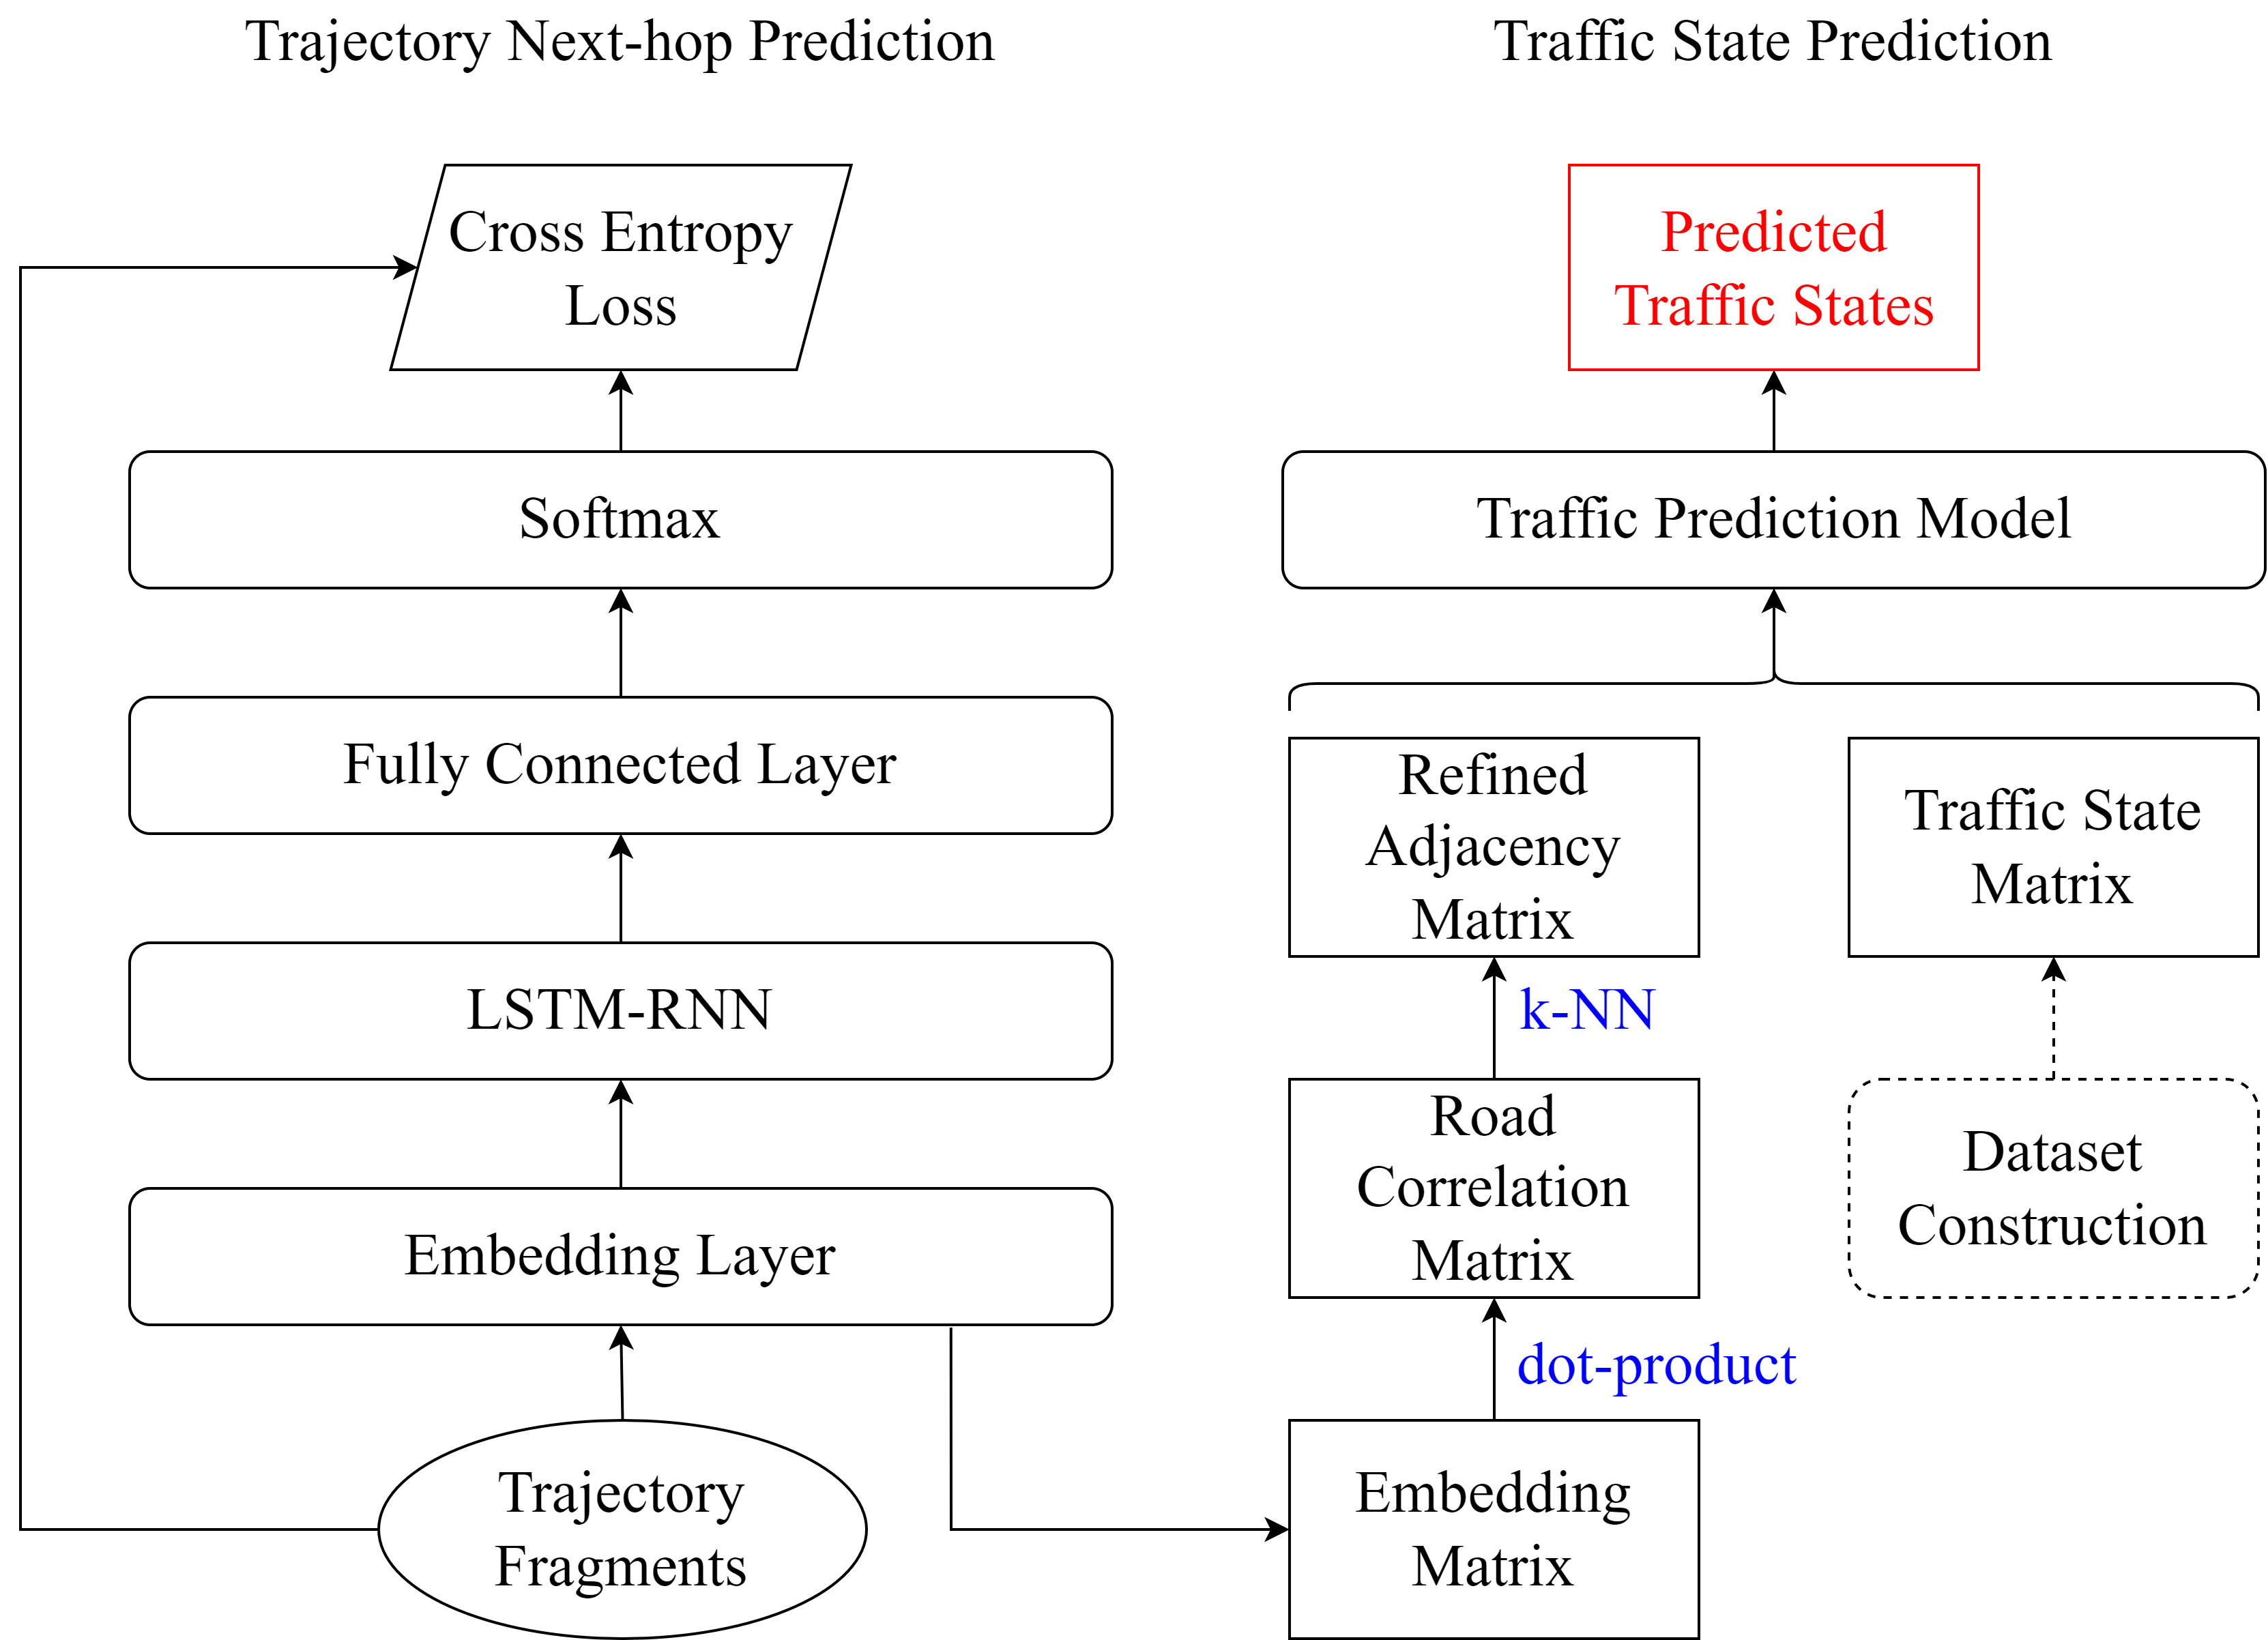
\includegraphics[width=\textwidth]{images/model.drawio.png}
    \caption{An overview of model structure.}
    \label{fig: model}
  \end{figure}

\subsection{Trajectory-based Road Correlation}
As mentioned in section 1, traffic states in real world varies over time. The traffic states in peak hours will even be completely different from other time intervals. However, most GCN models view the road network as a changeless graph, thus, they use adjacency matrix $A$ to represent it. On the contrary, trajectories indicate the route of vehicles, i.e. the real choices made by driver, which will give us the concrete transfer processes among roads. By leveraging them, we target to extract the road correspondence information inside transition and use a number to represent it. A simple way is regarding it as a first-order Markov process\cite{AAAI21}, and calculate the Markov transition probability as road correlation value by iterating on all trajectories. But Markov process is short in modeling high-order transition, since the next step is only related to the previous one, by its definition. Therefore, instead of statistical methods that result in a fixed probability value, we take advantage of deep leaning to let the machine automatically learn the transition process and output the high-order dependencies. To be specific, our idea is to build a trajectory next-hop prediction model and dynamically learn a vector representation of each road. Then compute vector similarity as road correlation. Details of methods and their rationale are introduced in the following paragraphs.

\vspace{\baselineskip}

\textbf{Migrating Word Embedding to Road Network Graph.} In NLP area, how to obtain the effective representations of text words has long been a research focus. One-hot embedding is a simple solution to represent each word with a one-hot vector whose dimension is equal to the size of vocabulary. The difference between these vectors are the word indexes. However, one-hot embedding suffers from dimension curse, making the embedding vectors very large and sparse. More importantly, the vectors cannot reflect the semantic relationships between words. Therefore, word embedding technologies\cite{word_embed} are proposed to efficiently learn a fixed-length real-value vector representation for each word. And the biggest advantage is that it can catch the contextual similarity of words. If two embedding vectors are close, i.e. have a high similarity, then the two corresponding words also tend to have similar semantic meanings.

In our work, a trajectory contains a sequence of different road IDs, which is similar to a sentence. Therefore, it is natural to treat each road as a word and use an embedding vector to represent it. What's more, we are inspired that road correlation can be modeled by the contextual similarity of words. To be specific, the similarity of words' semantic meanings ideally models the low and high-order dependency among roads, which perfectly meets the definition of road correlation. As a result, for road $r_1$, $r_2$ and their word embedding vectors $\mathbf{e_1}$ and $\mathbf{e_2}$, we define the road correlation function $Cor$ as the dot-product similarity\cite{dot_prod_simi} of the embedding vectors.
\begin{equation}
    Cor(r_1, r_2)=\mathbf{e_1}\cdot \mathbf{e_2}
\end{equation}

\vspace{\baselineskip}

\textbf{Next-hop Prediction Model}. To learn the embedding vectors, we propose a simple LSTM\cite{LSTM}-based model to predict the next-hop of a trajectory. Firstly, to utilize the trajectories, we use a sliding window strategy to generate training samples. After extracting the road sequence as $T^r=\{r_1, r_2, \dots, r_l \}$, we can obtain $l-w$ fragments by sliding a window with size $w$. A fragment is denoted as $\{r_1, r_2, \dots, r_w\}$, as well as its corresponding next-hop $r_{w+1}$. Next, we feed the fragments into an embedding layer that uses an embedding matrix $E\in\RR^{n_r\times d_r}$ to map each road ID to a vector of continuous values, where $n_r$ is the number of roads and $d_r$ is the embedding dimension. The second layer is an LSTM-RNN to capture dependencies in the sequence. LSTM encodes the embedded fragment into a single hidden vector with dimension $d_h$ after $w$ steps' iteration. The last layer is a fully connected linear layer that converts the hidden vector to an output length-$n_r$ vector for classification. Then use \textit{Softmax} function to generate the probability distribution. Cross entropy is served as loss function. The procedure of forward propagation is given in the following equations.
\begin{equation}
    \begin{aligned}
        \mathbf{e}&=\mathrm{Embedding}(r)\\
        h&=\mathrm{LSTM}(\mathbf{e})\\
        o&=W^\mathsf{T}h+b\\
        \hat P&=Softmax(o)\\
        \mathcal{L}&=CrossEntropy(\hat P, P)
    \end{aligned}
\end{equation}

After training, we take out the embedding matrix $E$ in the embedding layer and calculate the \textit{road correlation matrix} $C$ as
\begin{equation}
    C=E\cdot E^\mathsf{T}
\end{equation}
where $C_{i, j}=\mathbf{e_i}\cdot \mathbf{e_j}=Cor(r_i, r_j)$.

\subsection{Improving Traffic State Prediction}
Most state-of-the-art GCN models for traffic prediction take two inputs. One is traffic states, which is $X$ in our work. The other is graph adjacency matrix $A$ where information is shared and propagated along the edges. As stated in section 1, the advantage of correlation matrix is that it can reflect the dependencies among roads in real world, which is an improved version of adjacency. Therefore, instead of making a brand-new model, we decide to integrate road correlation matrix $C$ into the existing models to give them the correlation knowledge that will benefit in prediction. A naive thought is to replace adjacency matrix by road correlation matrix since they have the same shape $n_r\times n_r$. However, practice proves that this does not work well, and binary relations are still necessary. Therefore, we proposed a procedure to refine the adjacency matrix via the idea of $k$-nearest neighbors ($k$-NN)\cite{knn}. In detail, the semantic distance among roads can be represented by the distance of their embedding vectors, which is negatively related to the similarity, i.e. $distance(r_1, r_2)=-Cor(r_1, r_2)$. Therefore, finding the $k$ nearest neighbors of a road $r_i$ is equal to find the $k$ biggest correlation values' indices in the $i$-th row of road correlation matrix $C$. The \textit{refined adjacency matrix} $A'\in[0, 1]^{n_r\times n_r}$ will be determined as
\begin{equation}
    A'_{i, j}=\mathbb{I}(r_j\in k\mathrm{-NN}(r_i))=\mathbb{I}(j\in \mathrm{argsort}(C_i)_{:k})
\end{equation}
where $\mathbb{I}$ stands for the indicator function, $k\mathrm{-NN}$ generate a set of $k$ nearest neighbor roads, and $C_i$ is the $i$-th row of the correlation matrix. The order of $\mathrm{argsort}$ function is descending.

By replacing $A$ with $A'$, we improve the accuracy of traffic prediction models. The details of empirical verification is given in the next section.


\section{Experiments}
In this section, the details of training road embeddings by the next-hop prediction model will be given. And we will explain the process of parameter tuning. A verification for the functionality of road correlation, as well as an analysis and visualization are also stated in this section.

\subsection{Settings}
Our experiments were performed on a sever equipped with Intel(R) Xeon(R) Silver 4216 CPU @ 2.10GHz and an NVIDIA GeForce RTX 2080Ti graphics card. The PyTorch\cite{pytorch} version is 1.7.1 with Python 3.7.11.

\begin{table}[htb]
    \begin{center}
        \caption{Tuned parameters for next-hop prediction.}
        \label{next-hop_params}
        \begin{tabular}{clll}
            \toprule
  
            \textbf{Notation} & \textbf{Parameter} & \textbf{Search Space} & \textbf{Selected Value}\\
  
            \midrule
  
            $w$ & Window size & $\{5 \}$ & $5$\\
            $p$ & Sampling proportion & $\{0.05, 0.1, 0.2, 0.4, 0.8\}$ & $0.8$\\
            $d_r$ & Road embedding dimension & $\{16, 32, 64, 128 \}$ & $64$\\
            $d_h$ & LSTM hidden size & $\{32, 64, 128, 256 \}$ & $256$\\
            $d_o$ & Linear output dimension & $d_o=n_r=\#roads$ & $492$\\
            ~ & Batch size & $\{64, 128, 256, 512 \}$ & $256$\\
            ~ & Learning rate & $\{0.0001, 0.001\}$ & $0.0001$\\
            ~ & Early stopping epochs & $\{5, 10, 15\}$ & $10$\\
  
            \bottomrule
        \end{tabular}
    \end{center}
\end{table}

For the next-hop prediction model, the window size for trajectory fragments generation was set as $w=5$. After data processing, we got 1,751,602 trajectories in total. Removing too long and too short ones, there were 1,351,700 remaining. Then we put the trajectories into 24 bins according to their starting time and randomly sampled $p=80\%$ data in each bin to combine as the whole dataset. Finally, there were 1,076,886 trajectories. The data ratio for training, validation, and testing was set as 7:1:2. After window sliding, we got 10,228,578 trajectory fragments for training, and 1,455,100 for validation. Adam\cite{adam} algorithm was employed to control the overall training process, and the loss function was \textit{Cross Entropy Loss}. The complete parameter selection is given in table \ref{next-hop_params}.

For traffic state prediction models, the experiments were performed on DL-Traff\cite{dl-traff}, an open-source benchmark platform. As for the parameters, the input steps and prediction steps were both set to 12. The size of traffic state matrix is $n_r\times n_t=492\times 8064$. The data split ratio was also 7:1:2, and after sampling, we got 6437 traffic state vectors for training. The optimizer was Adam where the learning rate was set as 0.001, and the loss function was \textit{Mean Squared Error (MSE) Loss}. Batch size was set to 32 in order to avoid the \textit{CUDA Out of Memory} exception. Similarly, the training process would be early-stopped if the validation loss was not decreasing for 10 epochs, then the best model on validation data would be saved. Details are provided in table \ref{traff_pred_params}.

\begin{table}[htb]
    \begin{center}
        \caption{Parameters for traffic state prediction.}
        \label{traff_pred_params}
        \begin{tabular}{cll}
            \toprule
  
            \textbf{Notation} & \textbf{Parameter} & \textbf{Value}\\
  
            \midrule
  
            $w_{in}$ & Input steps & $12$\\
            $w_{out}$ & Prediction steps & $12$\\
            ~ & Batch size & $32$\\
            ~ & Learning rate & $0.001$\\
            ~ & Early stopping epochs & $10$\\
            ~ & Max training epochs & $200$\\
  
            \bottomrule
        \end{tabular}
    \end{center}
\end{table}

\subsection{Baseline Models}
We selected two baseline traffic prediction models that can effectively capture the spatial dependencies in the graph.

\begin{itemize}
    \item \textbf{HA} (Historical Average). Average the corresponding values from historical days as the prediction result.
    \item \textbf{CP} (Copy Last Steps). Directly copy the last one or multiple steps as the prediction result.
    \item \textbf{STGCN}\cite{STGCN} (Spatio-Temporal Graph Convolutional Networks). STGCN is proposed in 2018, which is one of the earliest spatiotemporal GCN models for traffic prediction. It uses gated TCN\cite{TCN} to capture temporal dependencies and applies spectral graph convolution\cite{GCN0} on graph to model the spatial dependencies.
    \item \textbf{DCRNN}\cite{DCRNN} (Diffusion Convolutional Recurrent Neural Network). DCRNN is another typical GCN model that is also proposed in 2018. Instead of spectral graph convolution, it implements diffusion convolution through bidirectional random walk to capture the transition information. Temporally, it integrates diffusion convolution into GRU and proposed an encoder-decoder structure to enable multistep prediction.
    \item \textbf{GWNET}\cite{GWNET} (Graph WaveNet). Graph WaveNet is a GCN model proposed in 2019, which still remains being one of the best SOTA models nowadays. It adopts adaptive/learnable graph rather than a static one that used in STGCN and DCRNN. By combining the original adjacency matrix and the learned graph, it can rapidly boost the prediction accuracy of traffic states.
\end{itemize}

We set the input graph as (1) \textit{adjacency matrix} $A$, (2) \textit{OD matrix} (3) \textit{Pearson correlation coefficient matrix of temporal features} $P$ (4) \textit{cosine similarity matrix of temporal features} (5) \textit{DTW distance of temporal features} (6) \textit{road correlation matrix} $C$ (7) \textit{refined adjacency matrix} $A'$ to compare their performance and illustrate the effect of road correlation in traffic state prediction. We give an ablation study by comparing the performance of $C$ and $A'$.

\subsection{Evaluation Metrics}
Following previous studies, we use \textit{Root Mean Square Error (RMSE)}, \textit{Mean Absolute Error (MAE)}, and \textit{Mean Absolute Percentage Error (MAPE)} as the metrics to show the performance of different methods. Zero values will be ignored, and lower errors indicate better performance. The definition of them are as following.

\begin{equation}
    \begin{aligned}
        MAE&=\frac 1n\sum_{i=1}^n|\hat{y_i}-y_i|\\
        MAPE&=\frac 1n\sum_{i=1}^n|\frac{\hat{y_i}-y_i}{y_i}|\\
        RMSE&=\sqrt{\frac 1n\sum_{i=1}^n(\hat{y_i}-y_i)^2}
    \end{aligned}
\end{equation}

\begin{table}[t!]
    \renewcommand\arraystretch{1.2} % line space
    \begin{center}
        \caption{Performance evaluation results.}
        \label{performance_results}
        \resizebox{\textwidth}{!}{
            \begin{tabular}{c|c|c|ccc|ccc|ccc}
                \toprule
                
                \multirow{2}{*}{Traffic State} & \multirow{2}{*}{Model} & Graph & \multicolumn{3}{c|}{3 Steps / 15 min} & \multicolumn{3}{c|}{6 Steps / 30 min} & \multicolumn{3}{c}{12 Steps / 60 min} \\

                \cline{4-12}

                                                 &                        & Type                    & RMSE       & MAE       & MAPE        & RMSE      & MAE       & MAPE        & RMSE       & MAE        & MAPE        \\
                \hline

                \multirow{23}{*}{Flow}           & HA                     & -                       & 5.84       & 4.35      & 41.18\%     & 5.82      & 4.34      & 41.10\%     & 5.8        & 4.33       & 40.98\%     \\
                                                 & CP                     & -                       & 7.23       & 5.37      & 50.13\%     & 7.23      & 5.38      & 50.15\%     & 7.24       & 5.38       & 50.16\%     \\
                \cline{2-12}
                                                 & \multirow{7}{*}{STGCN} & A                       & 4.44       & 3.46      & 33.00\%     & 4.64      & 3.57      & 33.64\%     & 5.07       & 3.88       & 36.07\%     \\
                                                 &                        & OD                      & 4.42       & 3.44      & 33.08\%     & 4.72      & 3.61      & 33.73\%     & 5.43       & 4.12       & 37.90\%     \\
                                                 &                        & P                       & 5.43       & 4.08      & 37.40\%     & 5.74      & 4.39      & 40.47\%     & 6.35       & 4.75       & 45.24\%     \\
                                                 &                        & COS                     & 5.43       & 4.08      & 37.40\%     & 5.74      & 4.39      & 40.47\%     & 6.35       & 4.75       & 45.24\%     \\
                                                 &                        & DTW                     & 4.39       & 3.4       & 32.40\%     & 4.63      & 3.57      & 33.70\%     & 5.03       & 3.82       & 35.73\%     \\
                                                 &                        & C                       & 4.38       & 3.4       & 32.41\%     & 4.56      & 3.52      & 33.33\%     & 5.03       & 3.82       & 35.87\%     \\
                                                 &                        & A'                      & 4.42       & 3.43      & 32.67\%     & 4.61      & 3.55      & 33.35\%     & 5.03       & 3.82       & 35.80\%     \\
                \cline{2-12}
                                                 & \multirow{7}{*}{DCRNN} & A                       & 4.47       & 3.46      & 33.01\%     & 4.66      & 3.6       & 34.06\%     & 5.03       & 3.85       & 35.76\%     \\
                                                 &                        & OD                      & 4.49       & 3.46      & 32.92\%     & 4.71      & 3.61      & 34.16\%     & 5.15       & 3.87       & 36.19\%     \\
                                                 &                        & P                       & 7.13       & 5.55      & 50.66\%     & 6.86      & 5.3       & 48.81\%     & 7.97       & 6.05       & 55.66\%     \\
                                                 &                        & COS                     & 4.42       & 3.42      & 32.71\%     & 4.6       & 3.53      & 33.46\%     & 5.01       & 3.79       & 35.35\%     \\
                                                 &                        & DTW                     & 11.11      & 8.83      & 76.44\%     & 11.9      & 9.9       & 89.60\%     & 12.56      & 10.58      & 97.62\%     \\
                                                 &                        & C                       & 8.19       & 6.13      & 55.66\%     & 8.18      & 6.13      & 55.64\%     & 8.13       & 6.09       & 55.33\%     \\
                                                 &                        & A'                      & 4.23       & 3.28      & 31.46\%     & 4.63      & 3.54      & 33.60\%     & 4.98       & 3.77       & 35.26\%     \\
                \cline{2-12}
                                                 & \multirow{7}{*}{GWNET} & A                       & 4.45       & 3.45      & 32.66\%     & 4.69      & 3.61      & 33.97\%     & 5.21       & 3.94       & 36.46\%     \\
                                                 &                        & OD                      & 4.51       & 3.48      & 32.76\%     & 4.78      & 3.65      & 34.04\%     & 5.45       & 4.07       & 36.81\%     \\
                                                 &                        & P                       & 4.31       & 3.34      & 32.00\%     & 4.58      & 3.51      & 33.44\%     & 4.93       & 3.73       & 34.93\%     \\
                                                 &                        & COS                     & 4.48       & 3.47      & 33.12\%     & 4.86      & 3.72      & 34.94\%     & 5.48       & 4.12       & 37.78\%     \\
                                                 &                        & DTW                     & 4.61       & 3.54      & 33.30\%     & 5.06      & 3.82      & 35.41\%     & 5.72       & 4.22       & 38.26\%     \\
                                                 &                        & C                       & 4.48       & 3.45      & 32.82\%     & 4.68      & 3.58      & 33.79\%     & 5.13       & 3.85       & 35.71\%     \\
                                                 &                        & A'                      & 4.41       & 3.41      & 32.61\%     & 4.57      & 3.51      & 33.31\%     & 4.98       & 3.76       & 35.25\%     \\
                \hline
                \hline

                \multirow{23}{*}{Speed}          & HA                     & -                       & 7.33       & 5.28      & 26.07\%     & 7.33      & 5.28      & 26.08\%     & 7.32       & 5.27       & 26.04\%     \\
                                                 & CP                     & -                       & 9.3        & 6.5       & 30.65\%     & 9.3       & 6.51      & 30.66\%     & 9.3        & 6.51       & 30.63\%     \\
                \cline{2-12}
                                                 & \multirow{7}{*}{STGCN} & A                       & 6.6        & 4.65      & 23.67\%     & 6.63      & 4.66      & 24.22\%     & 6.71       & 4.74       & 24.01\%     \\
                                                 &                        & OD                      & 6.61       & 4.66      & 23.64\%     & 6.62      & 4.67      & 24.05\%     & 6.71       & 4.76       & 24.14\%     \\
                                                 &                        & P                       & 6.6        & 4.64      & 23.61\%     & 7.28      & 5.36      & 27.06\%     & 6.5        & 4.56       & 24.30\%     \\
                                                 &                        & COS                     & 6.6        & 4.64      & 23.61\%     & 7.28      & 5.36      & 27.06\%     & 6.68       & 4.72       & 23.95\%     \\
                                                 &                        & DTW                     & 6.94       & 4.99      & 26.26\%     & 7.16      & 5.21      & 27.13\%     & 6.98       & 5.03       & 25.96\%     \\
                                                 &                        & C                       & 6.62       & 4.66      & 23.87\%     & 6.63      & 4.69      & 24.10\%     & 6.67       & 4.71       & 24.04\%     \\
                                                 &                        & A'                      & 6.6        & 4.65      & 23.66\%     & 6.63      & 4.68      & 24.04\%     & 6.67       & 4.72       & 24.00\%     \\
                \cline{2-12}
                                                 & \multirow{7}{*}{DCRNN} & A                       & 6.61       & 4.65      & 23.82\%     & 6.65      & 4.69      & 24.00\%     & 6.71       & 4.76       & 24.29\%     \\
                                                 &                        & OD                      & 6.83       & 4.87      & 25.04\%     & 7.02      & 5.07      & 25.37\%     & 7.3        & 5.33       & 26.64\%     \\
                                                 &                        & P                       & 6.59       & 4.64      & 23.80\%     & 6.63      & 4.67      & 23.95\%     & 6.67       & 4.73       & 24.17\%     \\
                                                 &                        & COS                     & 6.7        & 4.75      & 24.63\%     & 6.79      & 4.85      & 25.13\%     & 6.98       & 5.04       & 25.61\%     \\
                                                 &                        & DTW                     & 6.63       & 4.65      & 23.95\%     & 6.67      & 4.7       & 24.12\%     & 6.74       & 4.8        & 24.41\%     \\
                                                 &                        & C                       & 8.41       & 6.39      & 30.90\%     & 8.45      & 6.42      & 31.13\%     & 8.46       & 6.43       & 31.18\%     \\
                                                 &                        & A'                      & 6.62       & 4.65      & 23.82\%     & 6.66      & 4.68      & 23.99\%     & 6.71       & 4.75       & 24.25\%     \\
                \cline{2-12}
                                                 & \multirow{7}{*}{GWNET} & A                       & 6.84       & 4.84      & 25.51\%     & 7.06      & 5.06      & 27.07\%     & 7.88       & 5.82       & 31.48\%     \\
                                                 &                        & OD                      & 6.61       & 4.64      & 23.83\%     & 6.65      & 4.68      & 24.07\%     & 6.71       & 4.76       & 24.45\%     \\
                                                 &                        & P                       & 7.03       & 5.05      & 26.91\%     & 7.1       & 5.16      & 26.62\%     & 7.37       & 5.4        & 27.61\%     \\
                                                 &                        & COS                     & 6.62       & 4.65      & 23.85\%     & 6.66      & 4.69      & 24.15\%     & 6.74       & 4.78       & 24.75\%     \\
                                                 &                        & DTW                     & 6.62       & 4.66      & 23.82\%     & 6.66      & 4.7       & 24.06\%     & 6.72       & 4.77       & 24.52\%     \\
                                                 &                        & C                       & 6.62       & 4.67      & 23.65\%     & 6.65      & 4.7       & 23.77\%     & 6.71       & 4.78       & 24.00\%     \\
                                                 &                        & A'                      & 6.59       & 4.64      & 23.46\%     & 6.63      & 4.68      & 23.56\%     & 6.69       & 4.74       & 23.85\%     \\
                \bottomrule
            \end{tabular}
        }
    \end{center}
\end{table}

\subsection{Performance and Analysis}
First, we introduce the performance of the next-hop prediction model. We tried tens of parameter combinations and finally reached $5.47$ on test loss and $73.47\%$ on prediction accuracy. The embedding matrix $E$ in the model was saved for the computation of \textit{refined adjacency matrix} $A'$. Then the comparison of the traffic state prediction models' performance are given in table \ref{performance_results}. To demonstrate how the prediction accuracy varies with time, we report the metrics for 15, 30, 60-minutes ahead prediction. From the table, we obtain the following observations:

\begin{itemize}
    \item Our $A'$-version has the smallest error in almost every step for the three metrics, especially \textit{MAPE}. This illustrates that the proposed \textit{trajectory-based road correlation} can better capture the spatial dependencies on the road network graph than the adjacency matrix which cannot reflect the real world traffic scenarios.
    \item With the increasing of prediction steps, all models tend to perform worse because of the difficulty in long-range prediction. Coincidentally, the improvement of long-range metrics is also smaller than short-range. Compared to original $A$-version, our $A'$-version performs best in short-range prediction. For example, for 15-minutes ahead prediction, DCRNN-$A'$ has a $1.55\%$ lower \textit{MAPE} than DCRNN-$A$. But when turning to 60-minutes ahead, the improvement decreases to $0.5\%$. We think this is caused by the limitation of the next-hop model. In the last section, we mentioned that LSTM can capture high-order dependency. However, it is still incapable to catch the dependency for a 60-minutes duration. What's more, our choice for the window size $w=5$ may also lead to the short-sight of LSTM.
    \item STGCN is good at predicting traffic speed, while DCRNN is expert in traffic flow prediction. However, the difference between them in speed prediction is not as large as flow. The reason is that our \textit{trajectory-based road correlation} captures the road transition information, which is directly related to the propagation of traffic flow, but have nothing to do with the variation of traffic speed.
    \item \textbf{Ablation Experiment.} Our aim is to check the contribution of adjacency matrix refinement to the final performance. For the ablation study, we build the models STGCN-$C$ and DCRNN-$C$ that directly take correlation matrix $C$ as input. For STGCN, the results show that the $A'$-version is better in almost all cases. But what we want to emphasize is that the refinement process is essential for DCRNN. The table shows that DCRNN-$C$ performs very bad, such as the $55\%$ \textit{MAPE} for traffic flow prediction. In addition, when training the model, we found that the training loss is always increasing, i.e. the model cannot converge. This indicates that the diffusion convolution can only take binary relations as input. Therefore, it is necessary to use \textit{refined adjacency matrix} as DCRNN's input.
\end{itemize}

\subsection{Parameter Study}
\begin{figure}[htb]
    \centering
    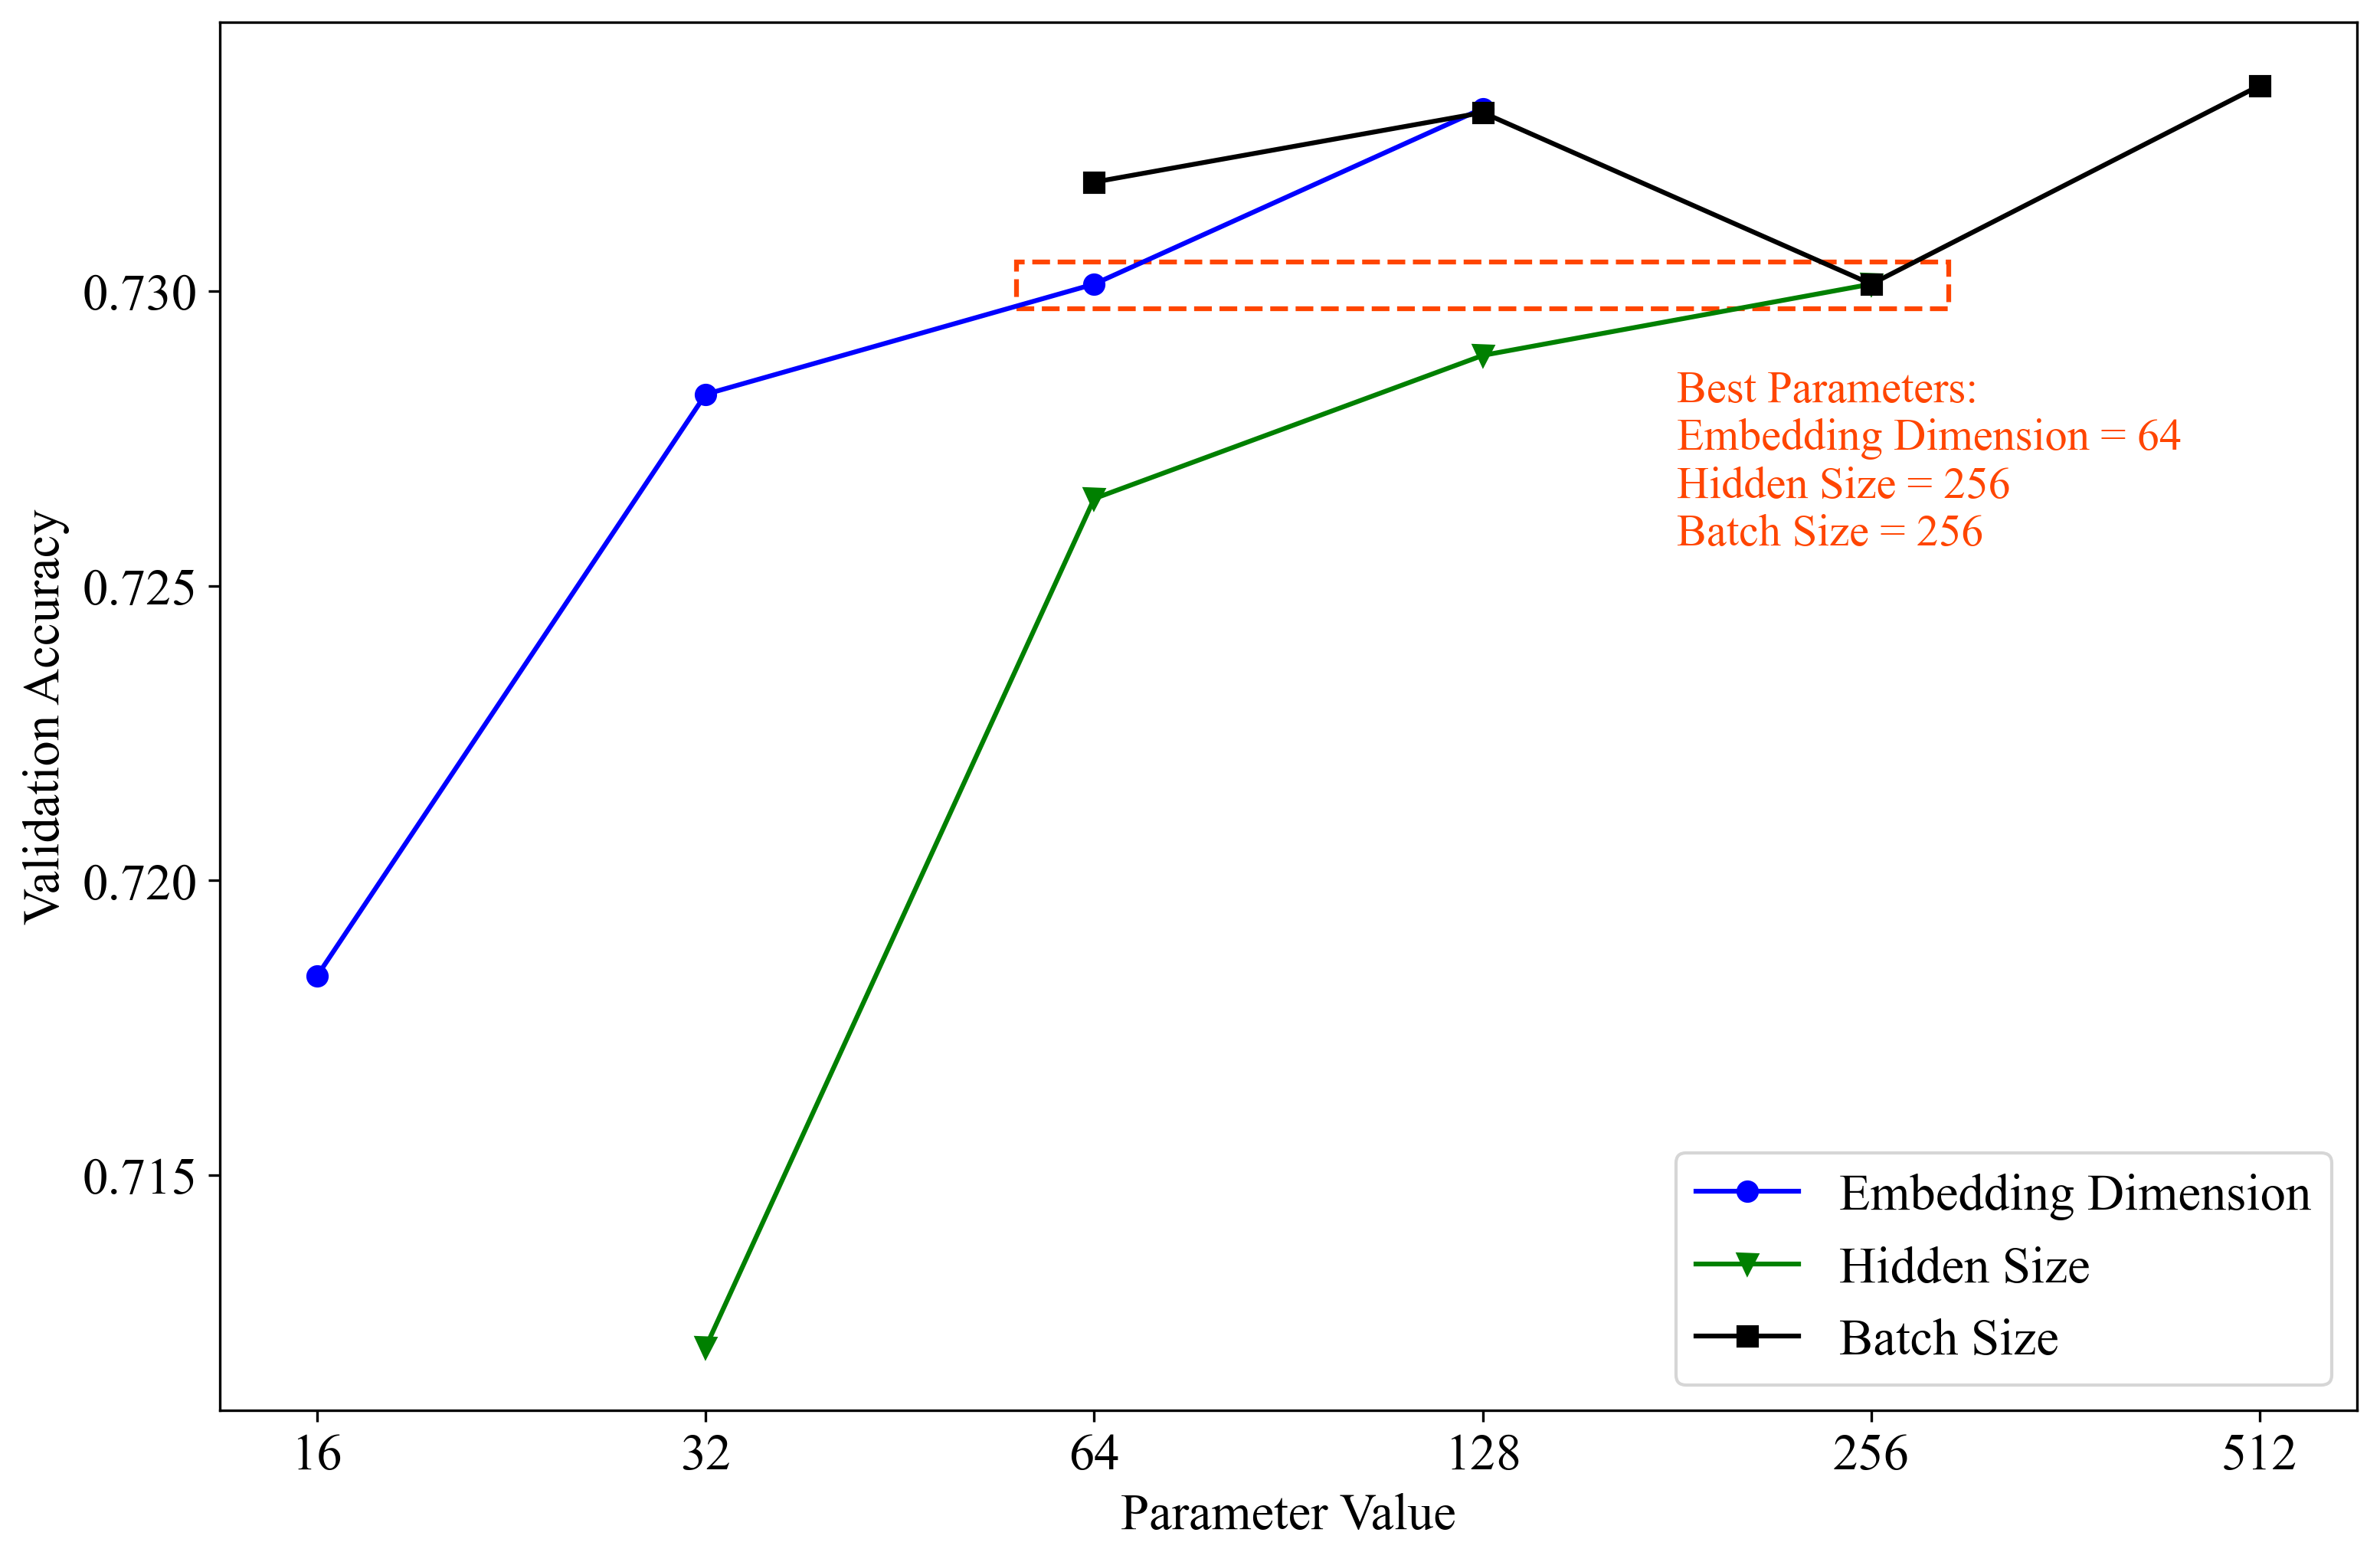
\includegraphics[width=\textwidth]{images/next-hop_param.png}
    \caption{Parameter tuning for the next-hop prediction model.}
    \label{fig: next-hop_param}
\end{figure}

This section introduces parameter analysis to provide a closer insight into our models. At first, the parameter tuning process of the next-hop prediction model is given in figure \ref{fig: next-hop_param}, including the choices for road embedding dimension, LSTM hidden size and batch size. The parameter search candidates are given in the above table \ref{next-hop_params} in section 6.1. Actually, according to the table, tuning these three parameters needs to search $4^3=64$ combinations, and should be plotted in a 3-D chart. But for the convenience of drawing, we set other two parameters fixed when studying one of them. The figure shows the variation of the prediction accuracy on validation dataset with parameter values. From it, we observe that (1) the prediction accuracy is positively related to embedding dimension and LSTM hidden size, because they become more representative. (2) Batch size has no clearly positive or negative relation with accuracy, needing case-to-case analysis. (3) Large embedding dimension and LSTM hidden size combinations will lead to lower accuracy, which is not displayed in the figure. Nevertheless, it is still necessary to be emphasized. Finally, considering the overall performance and the ability of generalization, we choose the parameters shown in the orange rectangle with $73.01\%$ prediction accuracy.

\begin{figure}[htb]
    \centering
    \caption{Variation of STGCN-$A'$ prediction \textit{MAPE} with $k$.}
    \label{fig: k}
    \begin{subfigure}[t]{0.49\linewidth}
        \centering
        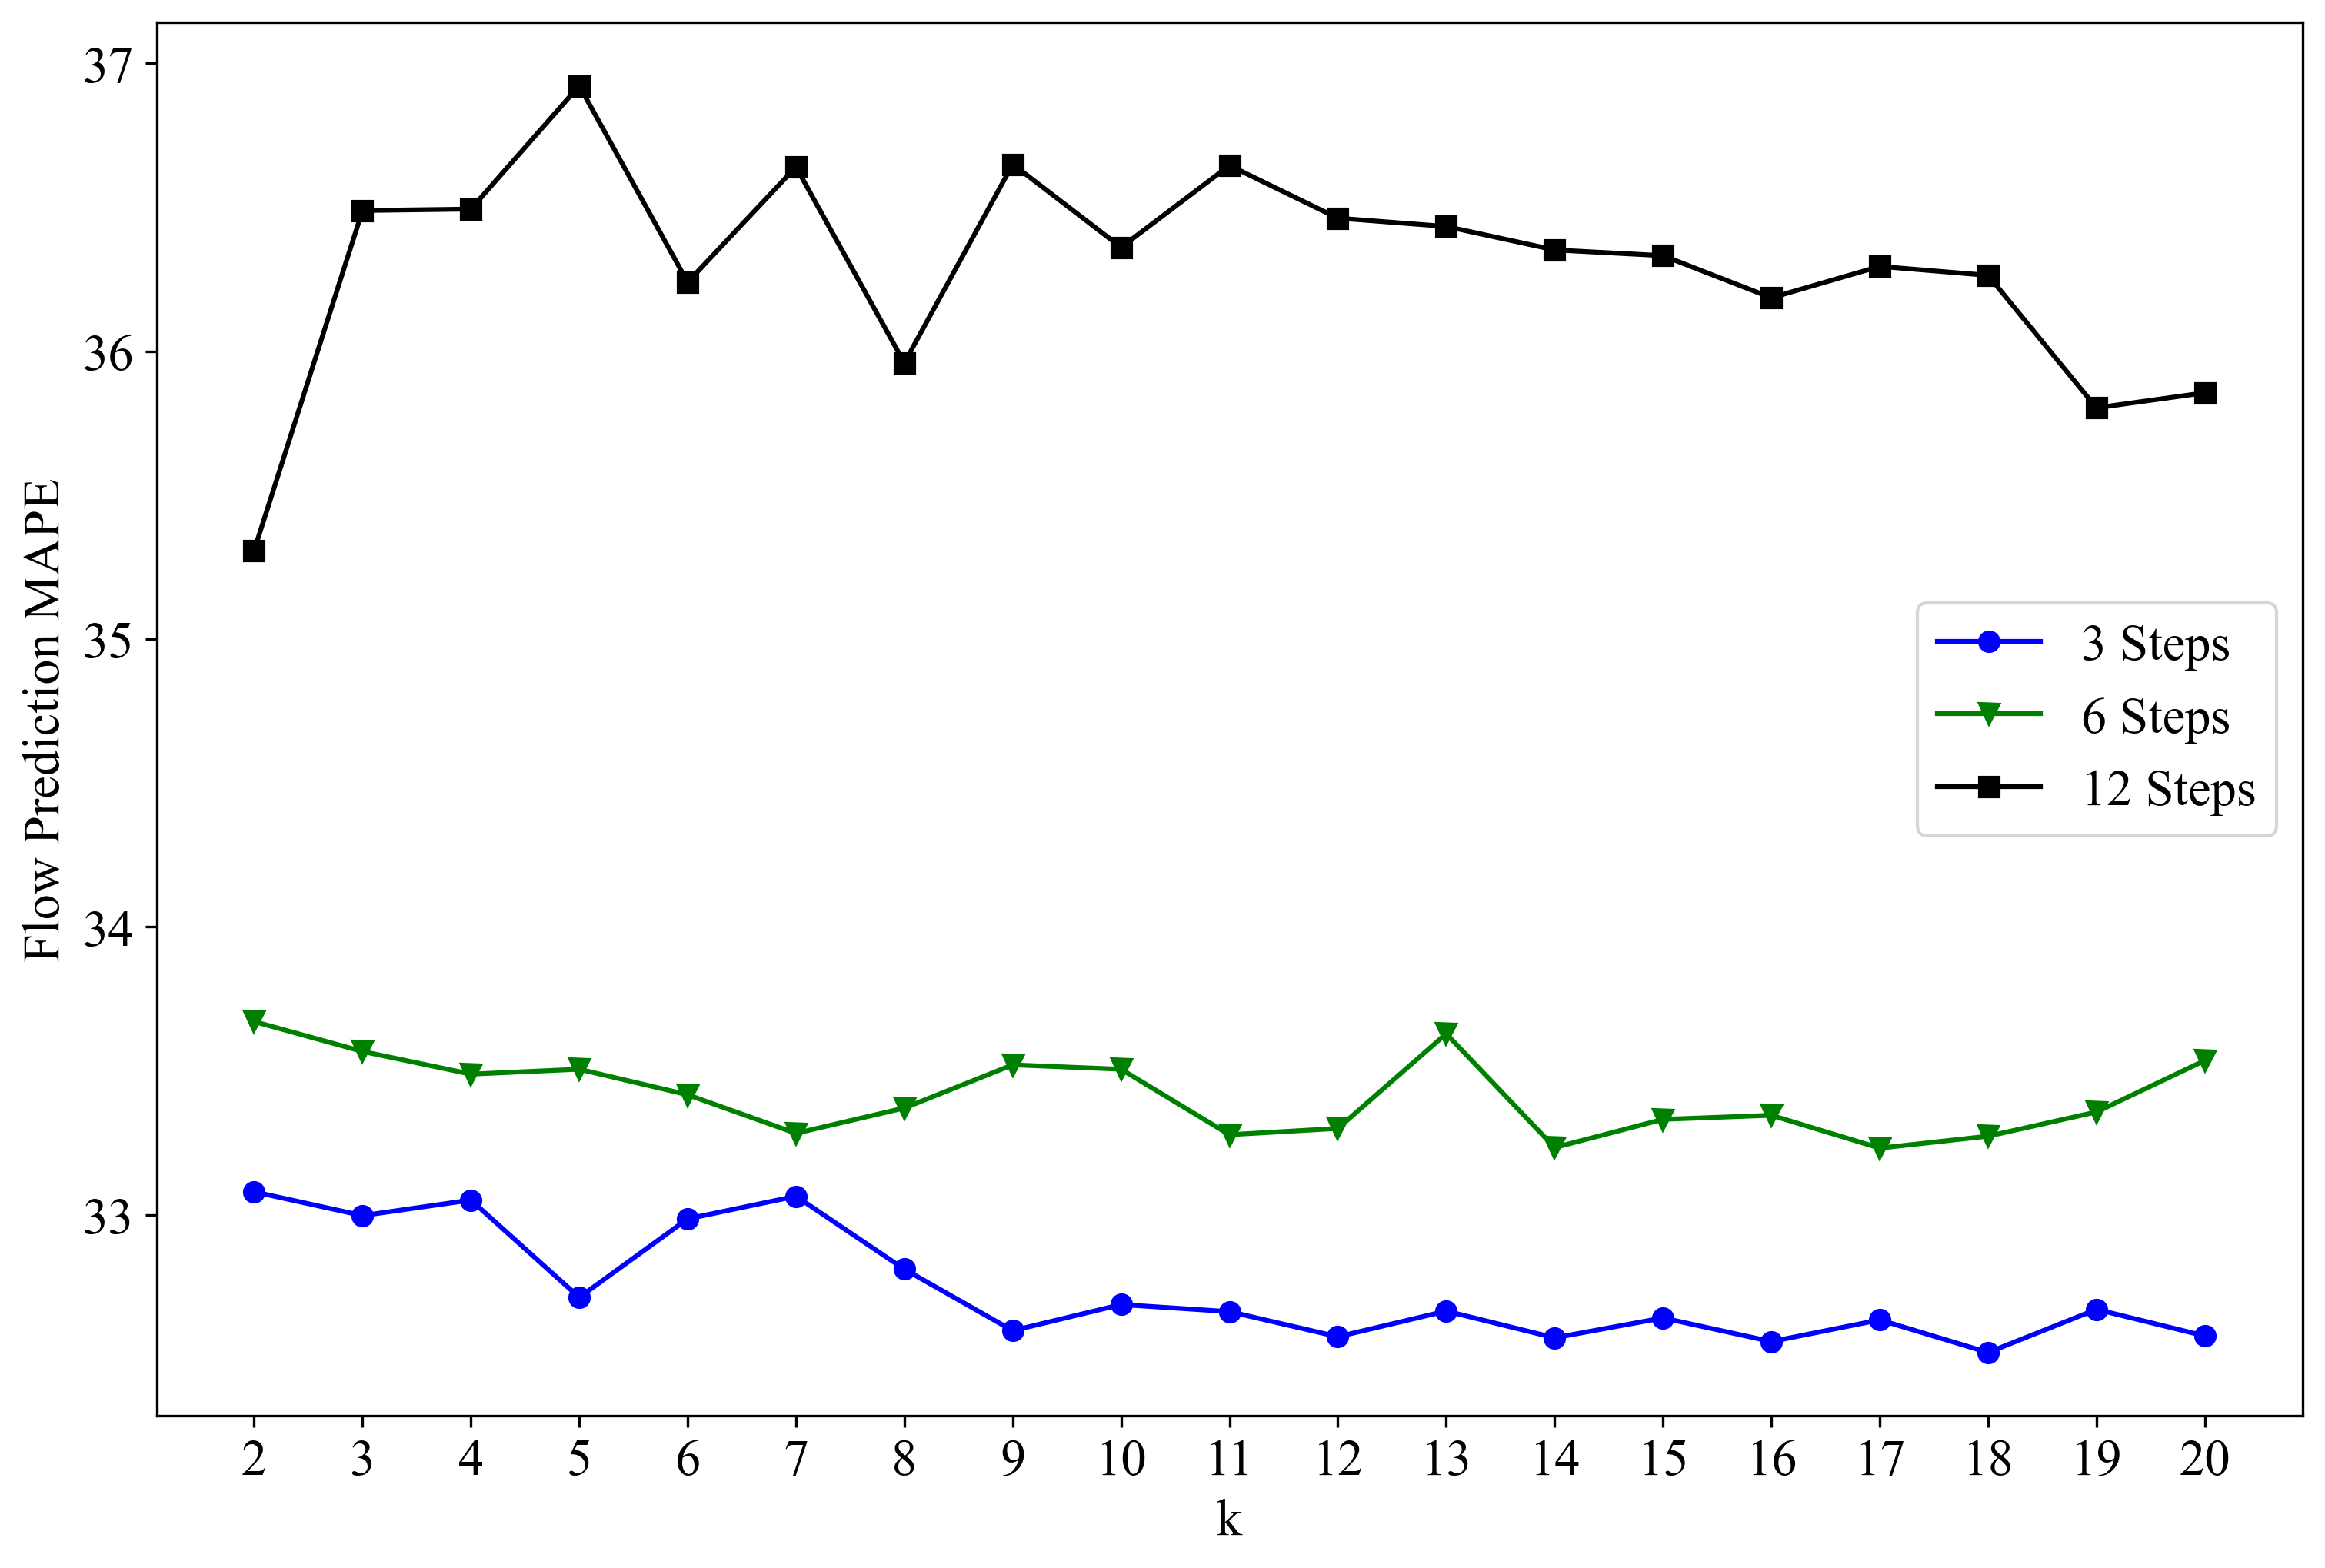
\includegraphics[width=\textwidth]{images/k-flow.png}
        \caption{Traffic flow prediction}
        \label{fig: k-flow}
    \end{subfigure}
    \begin{subfigure}[t]{0.49\linewidth}
        \centering
        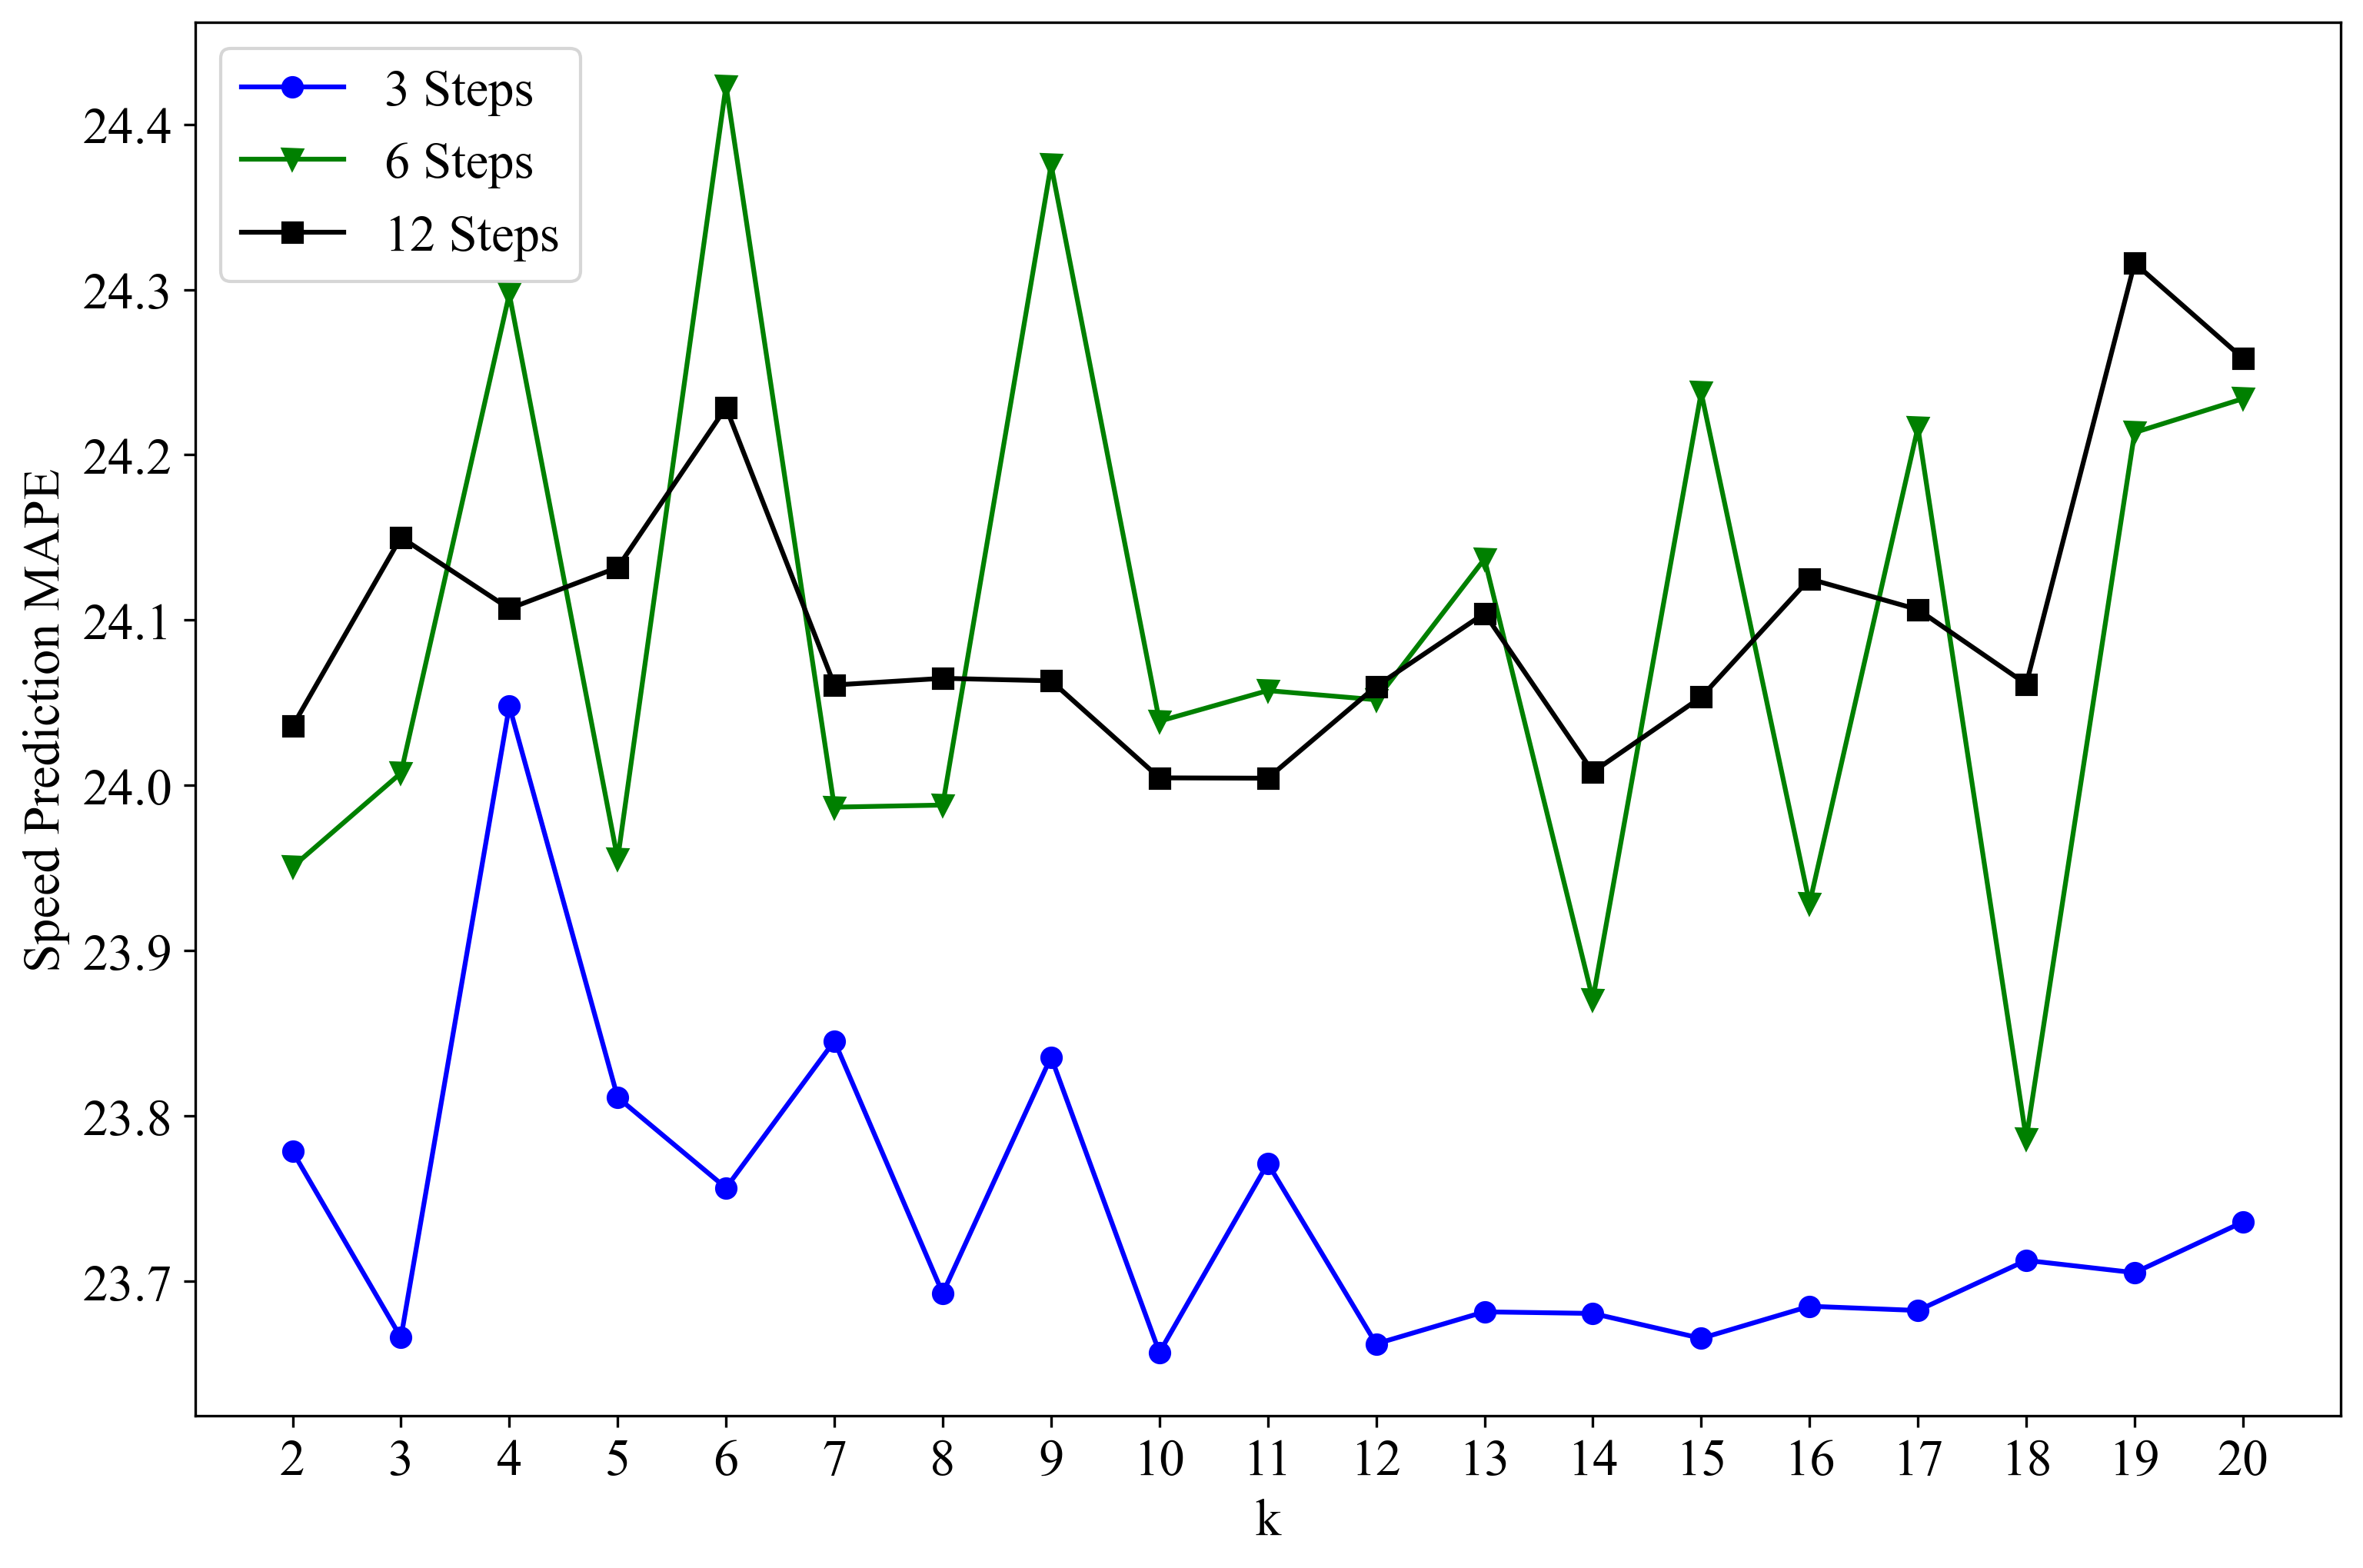
\includegraphics[width=\textwidth]{images/k-speed.png}
        \caption{Traffic speed prediction}
        \label{fig: k-speed}
    \end{subfigure}
\end{figure}
Secondly, we analyze the choice of $k$ when calculating \textit{refined adjacency matrix} $A'$. As shown in figure \ref{fig: k}, the prediction \textit{MAPE} changes randomly with the increase of $k$ from $2$ to $20$. Because the value in $A'$ is either zero or one, a small change can lead to totally different results. There is no general rule for us to determine the value of $k$. Therefore, according to the figure, we choose different $k$ for each step's prediction, which are given in table \ref{k_table}.
\begin{table}[htb]
    \renewcommand\arraystretch{1.5} % 1.5 line space
    \begin{center}
        \caption{The choices of $k$ for $A'$ generation.}
        \label{k_table}
        \begin{tabular}{c|c|c}
            \toprule
  
            \textbf{Model} & \textbf{Traffic State} & \textbf{$k$}\\
  
            \hline
  
            \multirow{2}{*}{STGCN-$A'$} & Flow & $19$\\
            \cline{2-3}
            ~ & Speed & $10$\\

            \hline

            \multirow{2}{*}{DCRNN-$A'$} & Flow & $8$\\
            \cline{2-3}
            ~ & Speed & $10$\\

            \hline

            \multirow{2}{*}{GWNET-$A'$} & Flow & $6$\\
            \cline{2-3}
            ~ & Speed & $11$\\
  
            \bottomrule
        \end{tabular}
    \end{center}
\end{table}

\subsection{Road Correlation Case Study}
In this section, we give a visualization for road correlation and select a specific road for a case study. At first, figure \ref{fig: heatmap} provides the heatmap of road correlations among $r_{225}$ to $r_{245}$. We selected these roads due to the space limitation. In the figure, the correlation values are normalized by MinMax normalization algorithm, and shown as a color block in the heatmap. Some rows have more high-value blocks compared to others. For example, row 241 and row 242. It indicates that some roads have high correlations with most roads in the road network. Referring to figure \ref{fig: gps_seq} and figure \ref{fig: road_correlation_map}, it can be seen that $r_{241}$ and $r_{242}$ are main roads of this district, which confirms our observation.

\begin{figure}[htb]
    \centering
    \caption{Visualization of road correlations.}
    \label{fig: vis_road_cor}
    \begin{subfigure}[t]{0.33\linewidth}
        \centering
        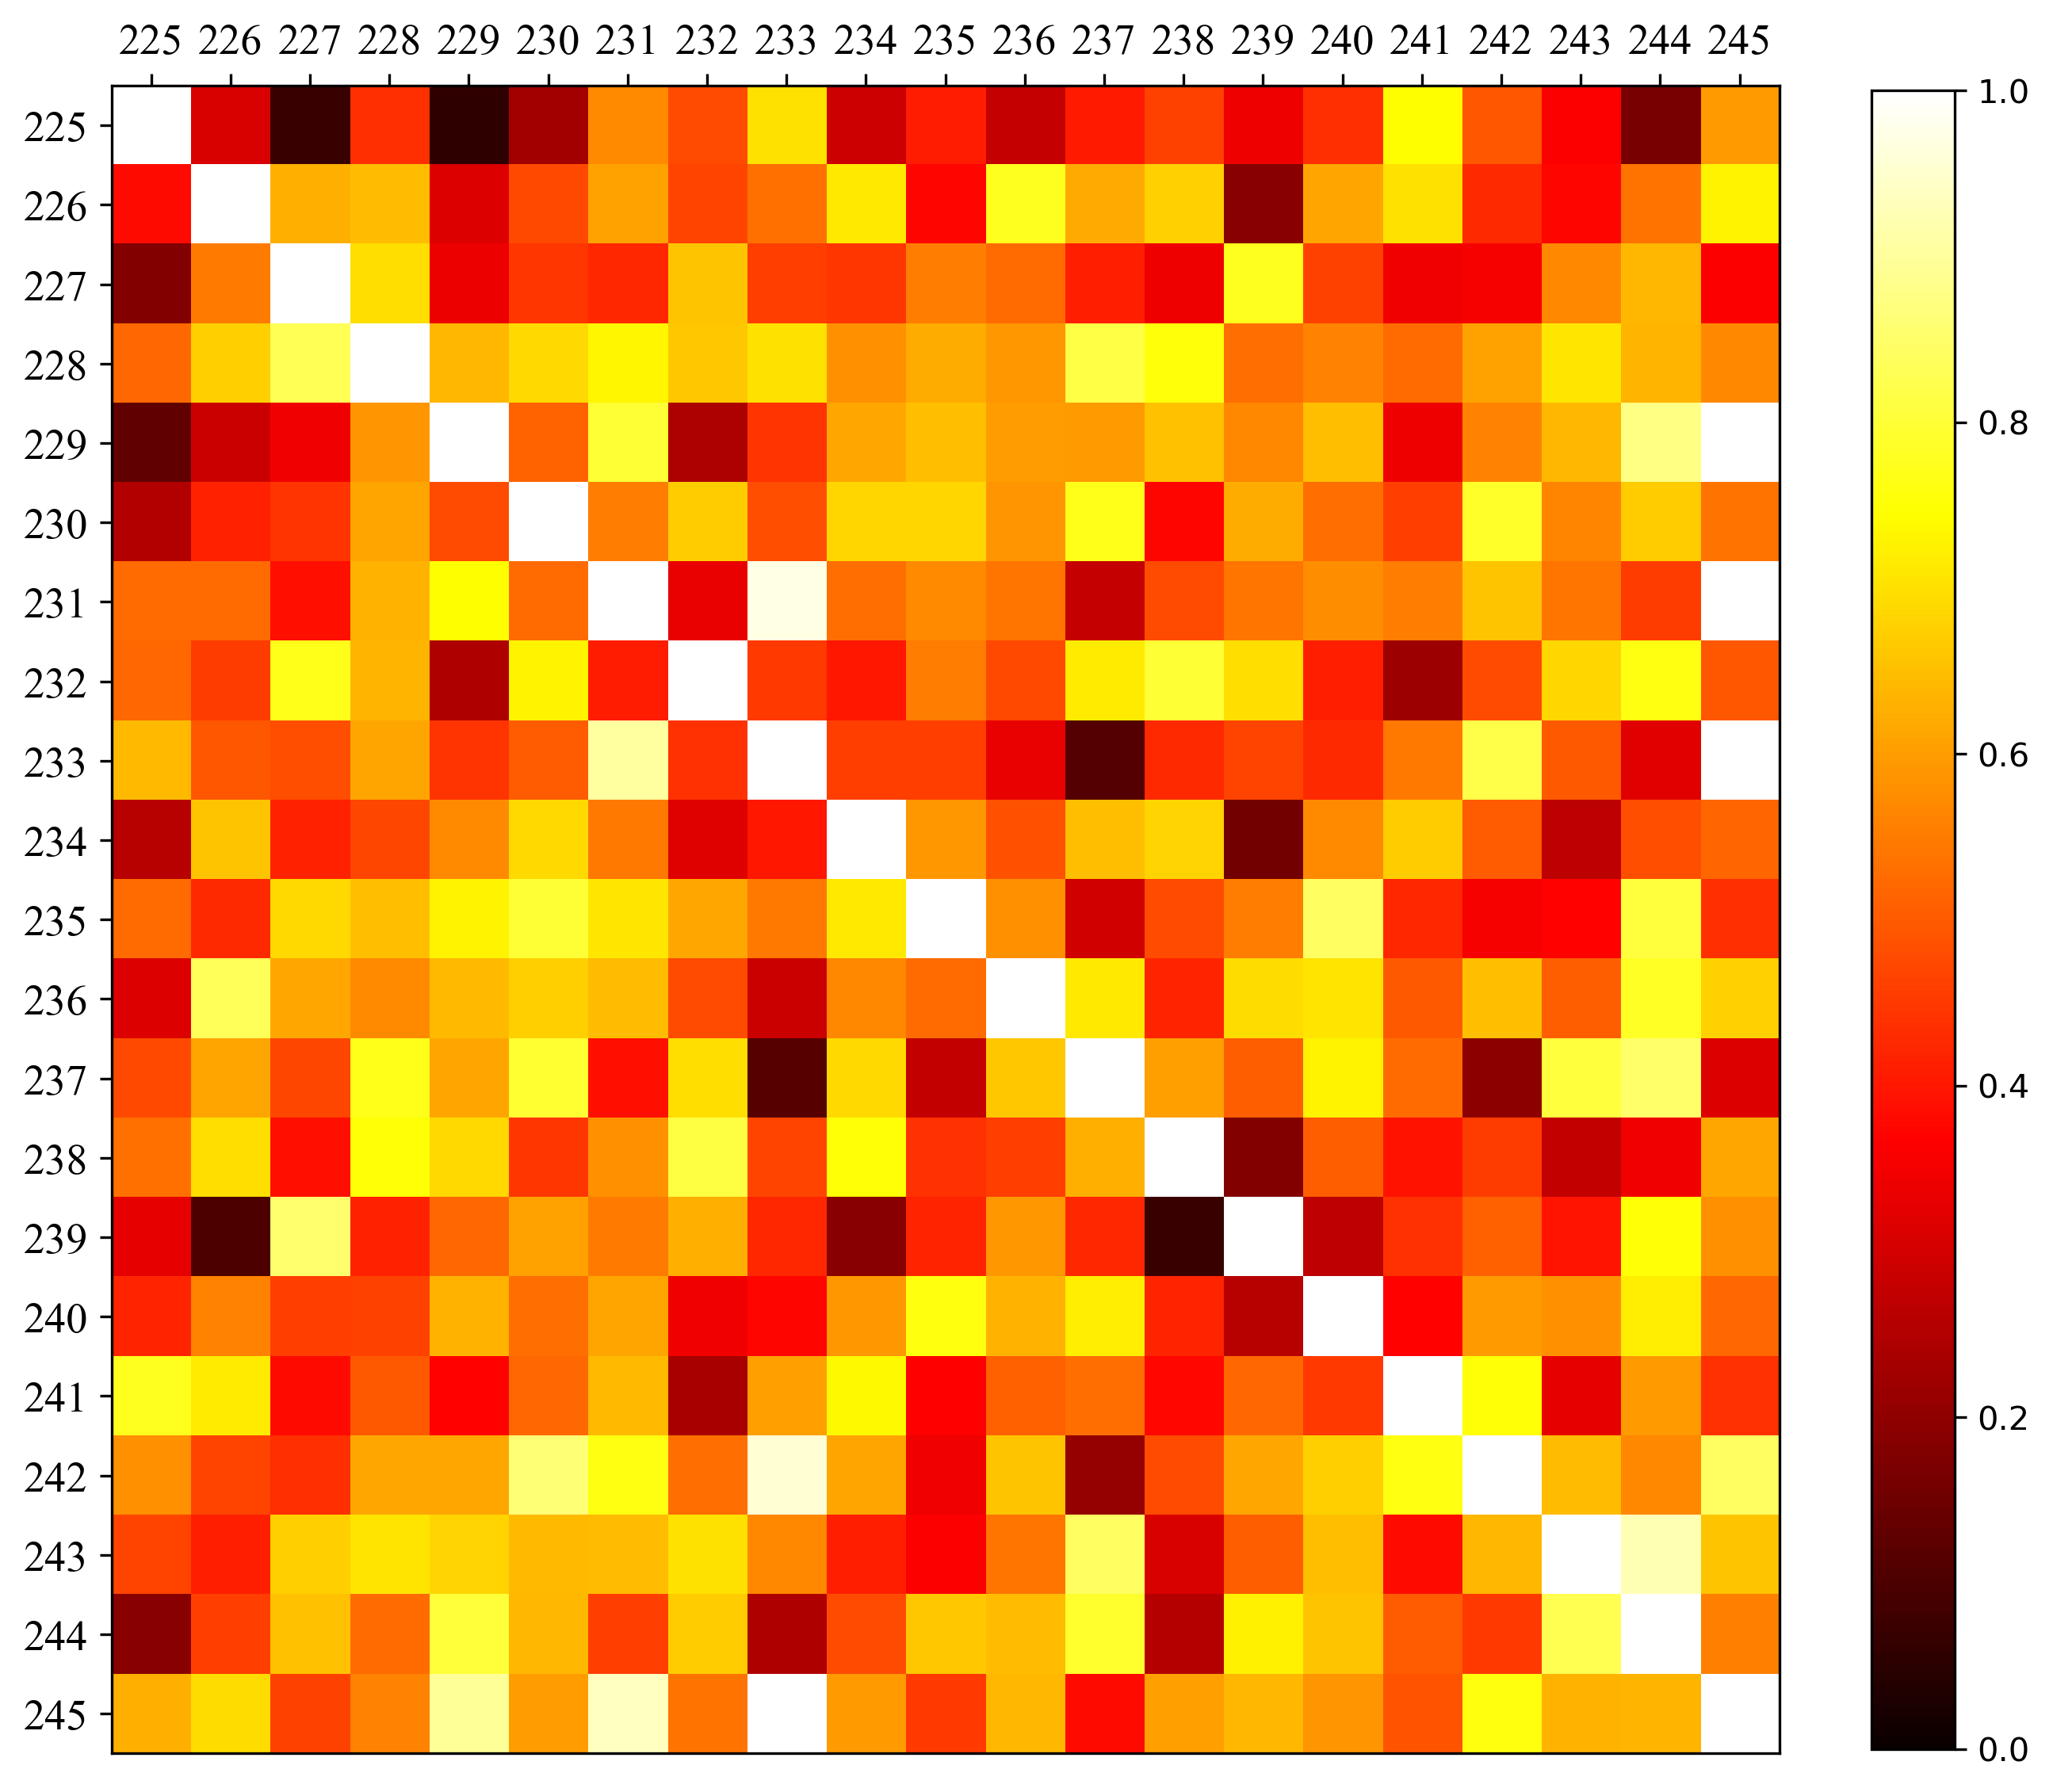
\includegraphics[width=\textwidth]{images/heatmap.png}
        \caption{Heatmap}
        \label{fig: heatmap}
    \end{subfigure}
    \begin{subfigure}[t]{0.66\linewidth}
        \centering
        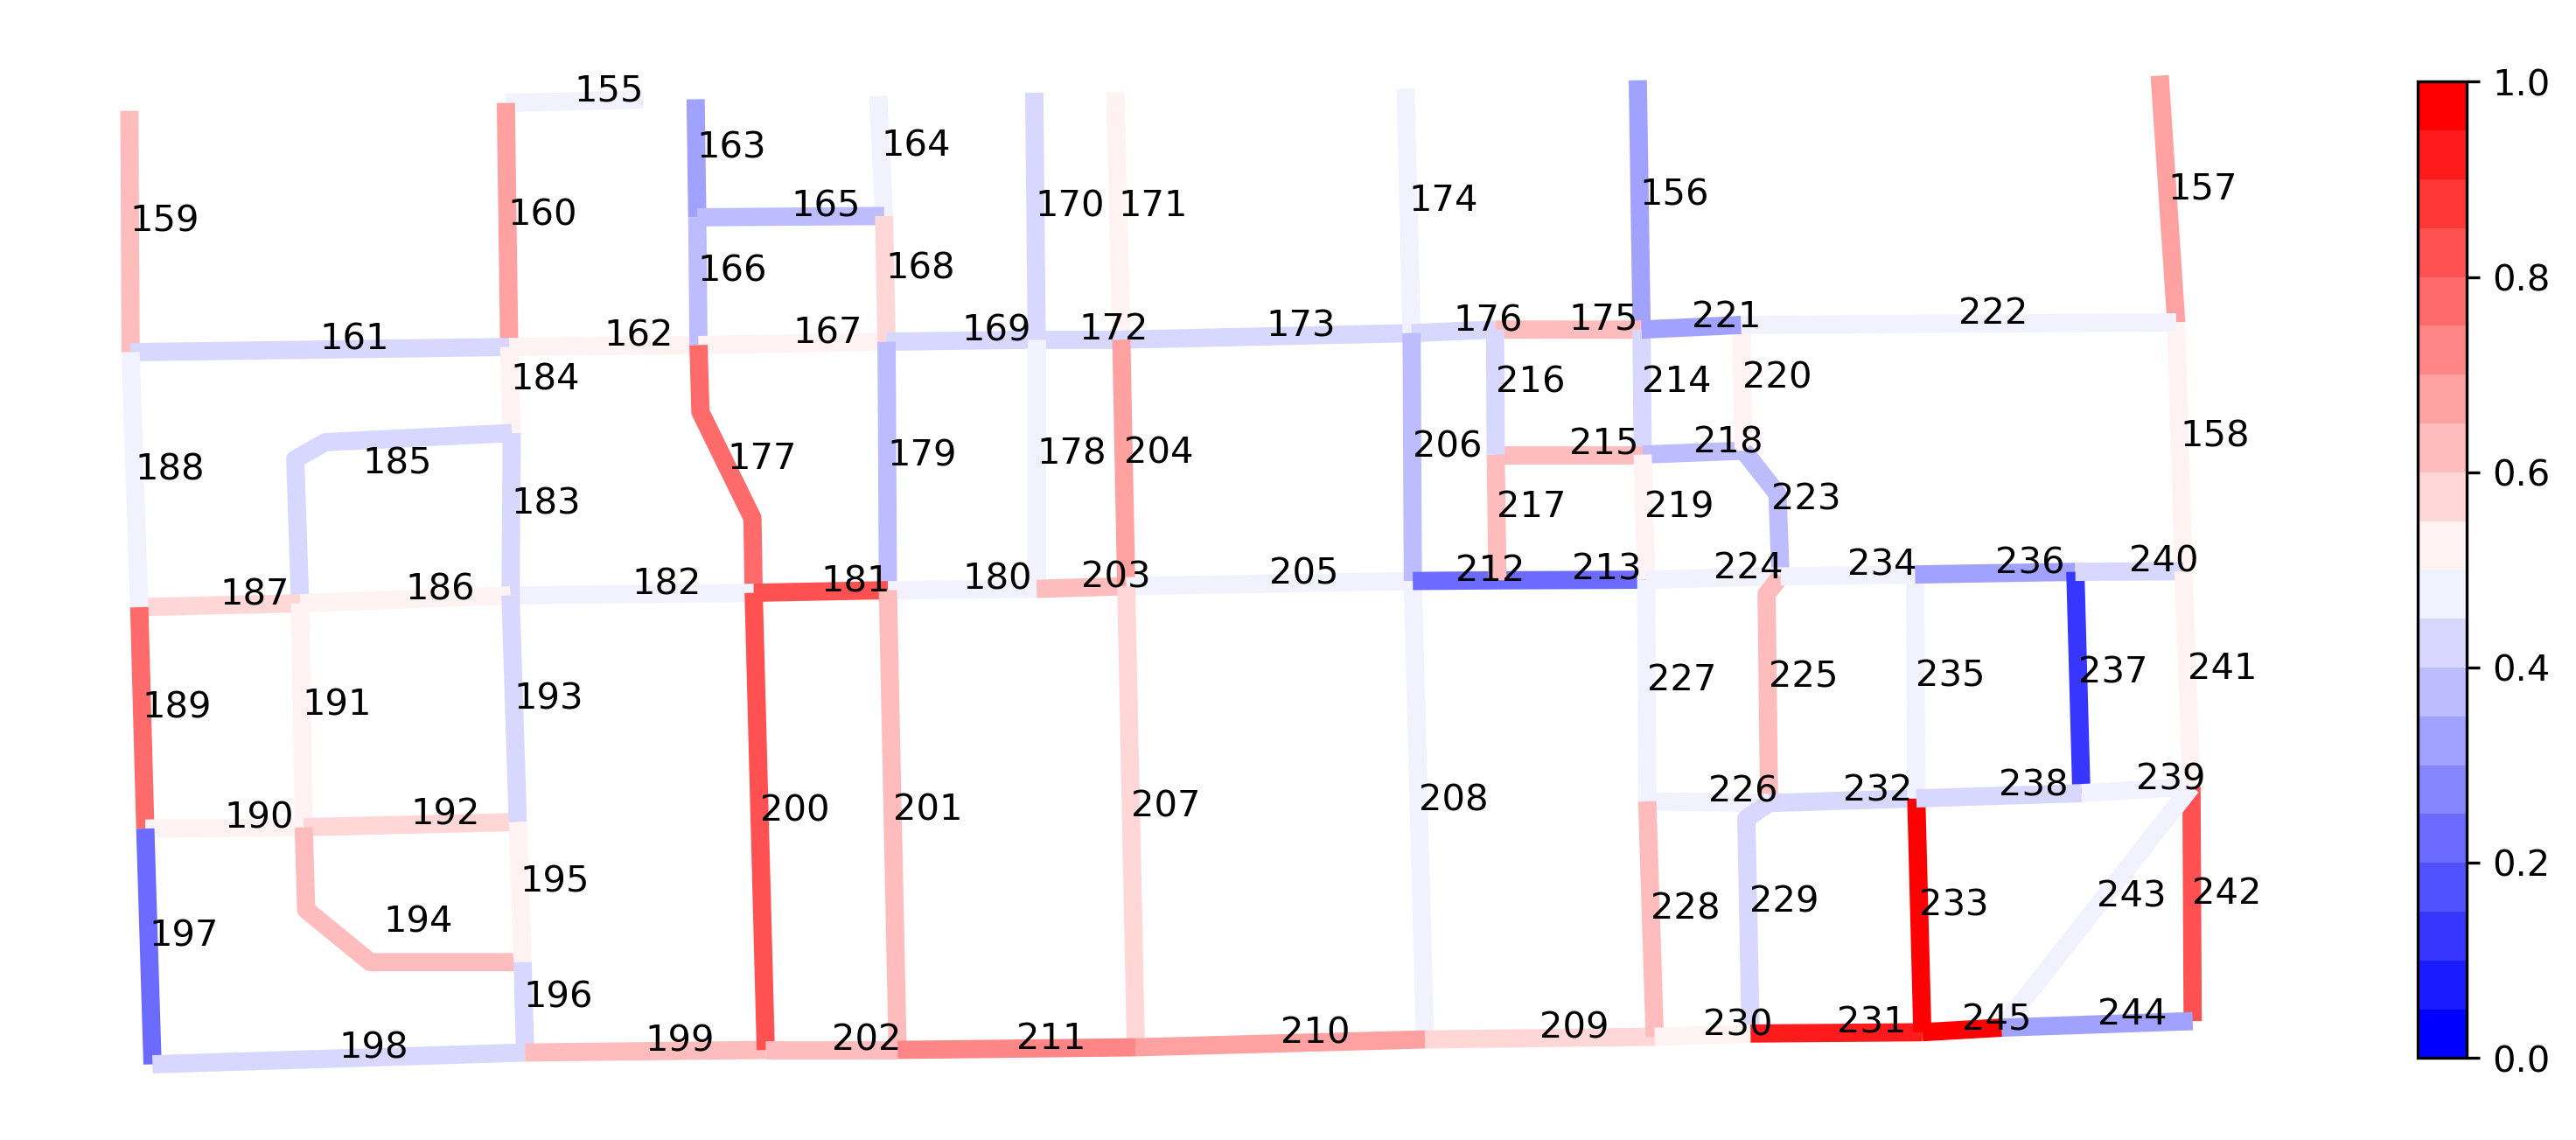
\includegraphics[width=\textwidth]{images/road_correlation.png}
        \caption{Road correlations of $r_{233}$ on map}
        \label{fig: road_correlation_map}
    \end{subfigure}
\end{figure}

% \begin{figure}[htb]
%     \centering
%     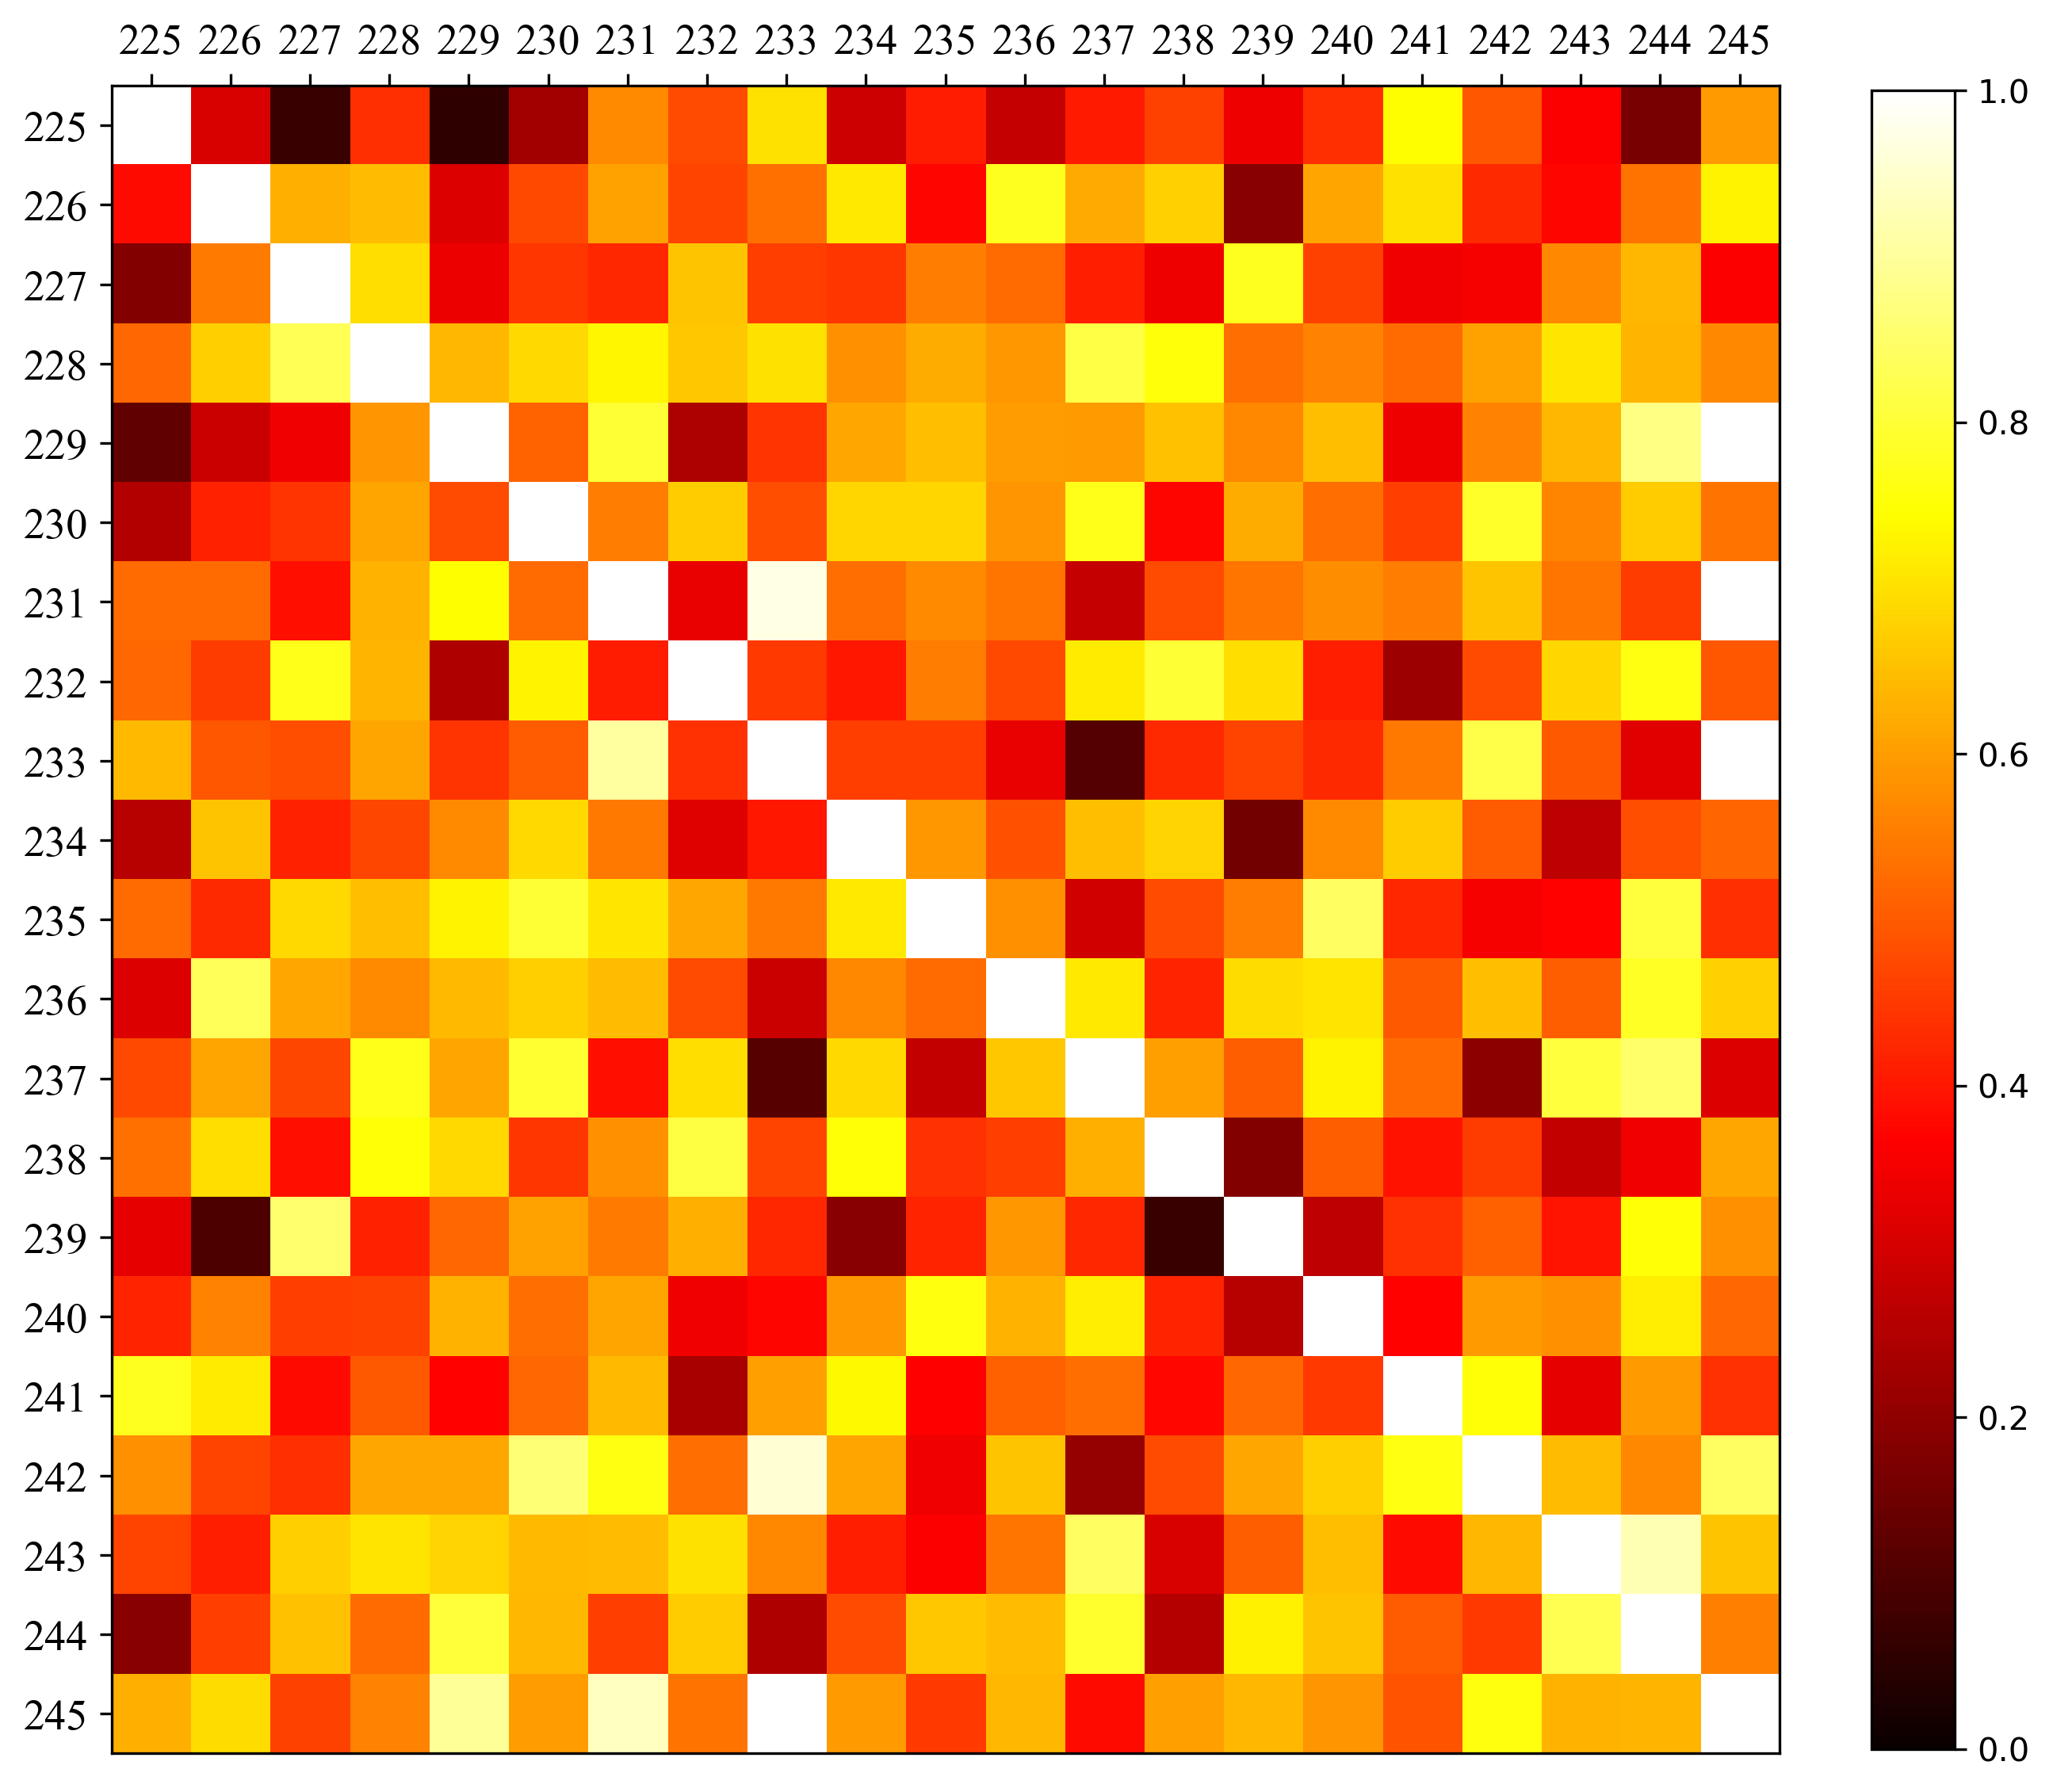
\includegraphics[width=\textwidth]{images/heatmap.png}
%     \caption{Road correlations heatmap.}
%     \label{fig: heatmap}
% \end{figure}

For the visualization on road network, we select roads $r_{155}$ to $r_{245}$, in total 91 roads, which lie in the bottom half of the road network, to visualize the road correlations among them. The road correlation values are taken directly from \textit{road correlation matrix} $C$, which is also the same as the row 233 in the heatmap. As a result, the figure \ref{fig: road_correlation_map} shows the correlations of road $r_{233}$ with other roads. The red road in the bottom right corner stands for $r_{233}$, while other roads are drawn by the color bar according to their correlation values. A redder color means that the corresponding road has a higher correlation with $r_{233}$, and vice versa. If a road is pure blue in the figure, then it has no correlation with $r_{233}$ at all. From the figure, we can observe that the nearby roads, which are $r_{231}, r_{245}, r_{242}, \dots$, are highly correlated with $r_{233}$. It meets our expectation because according to the map, they are $r_{233}$'s upstream and downstream roads, which means our model successfully captured the low-order dependencies. What's more, some long distance roads, such as $r_{200}, r_{181}, r_{177}$, also have considerable correlations with $r_{233}$, which are the high-order dependencies captured by the model. In short, the figure proves that the low and high-order spatial dependencies are both captured by our next-hop prediction model.

% \begin{figure}[htb]
%     \centering
%     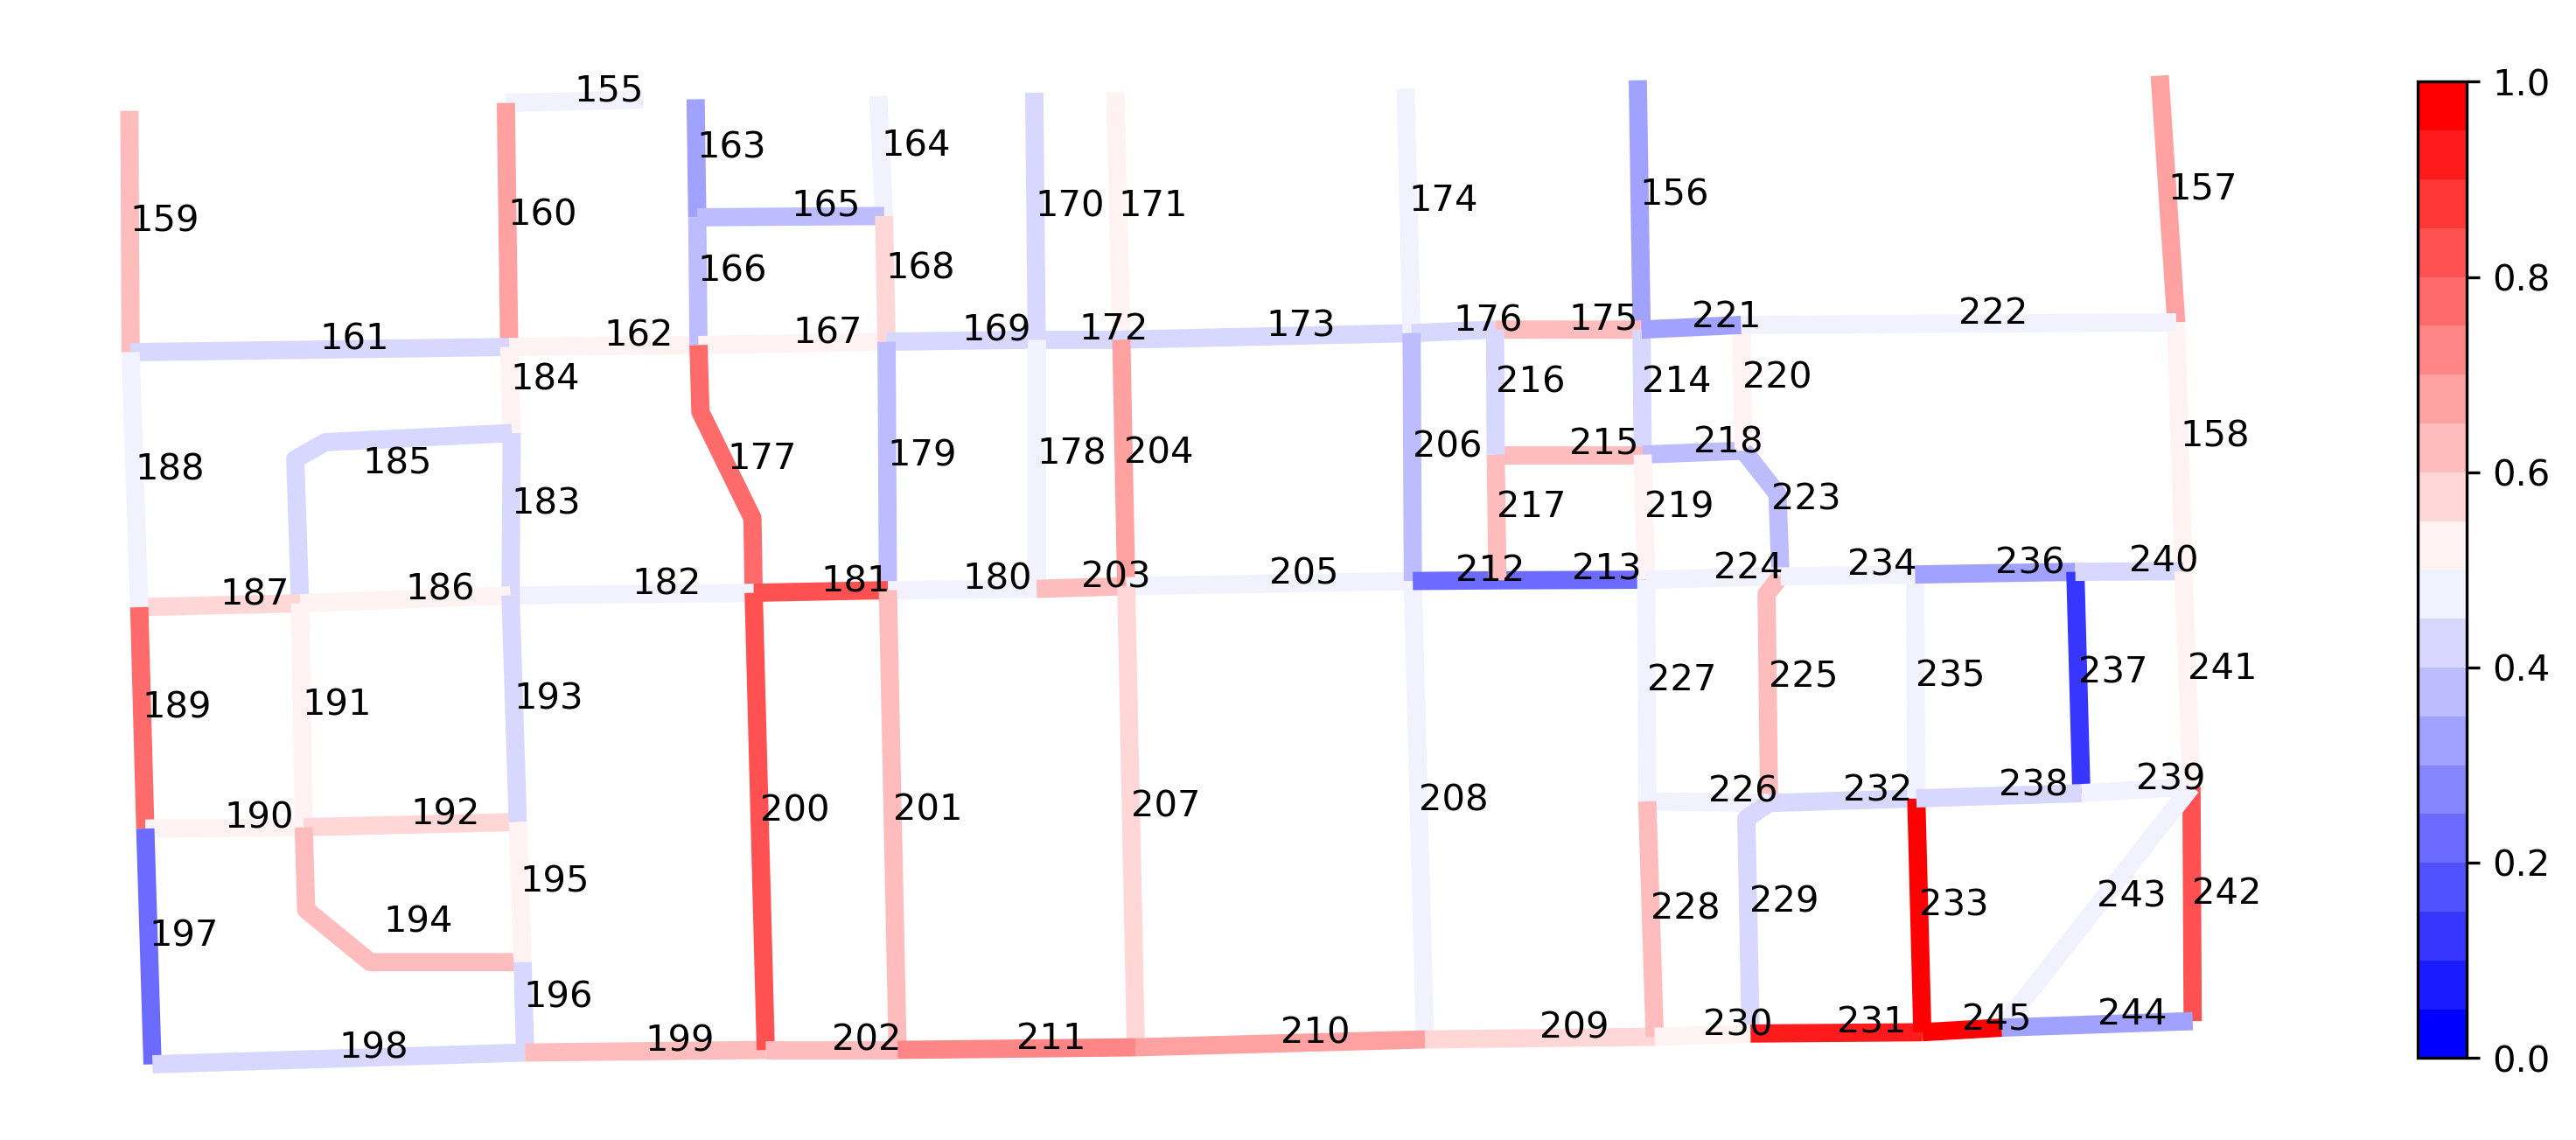
\includegraphics[width=\textwidth]{images/road_correlation.png}
%     \caption{Visualization for road correlations of $r_{233}$.}
%     \label{fig: road_correlation_map}
% \end{figure}

\begin{figure}[htb]
    \centering
    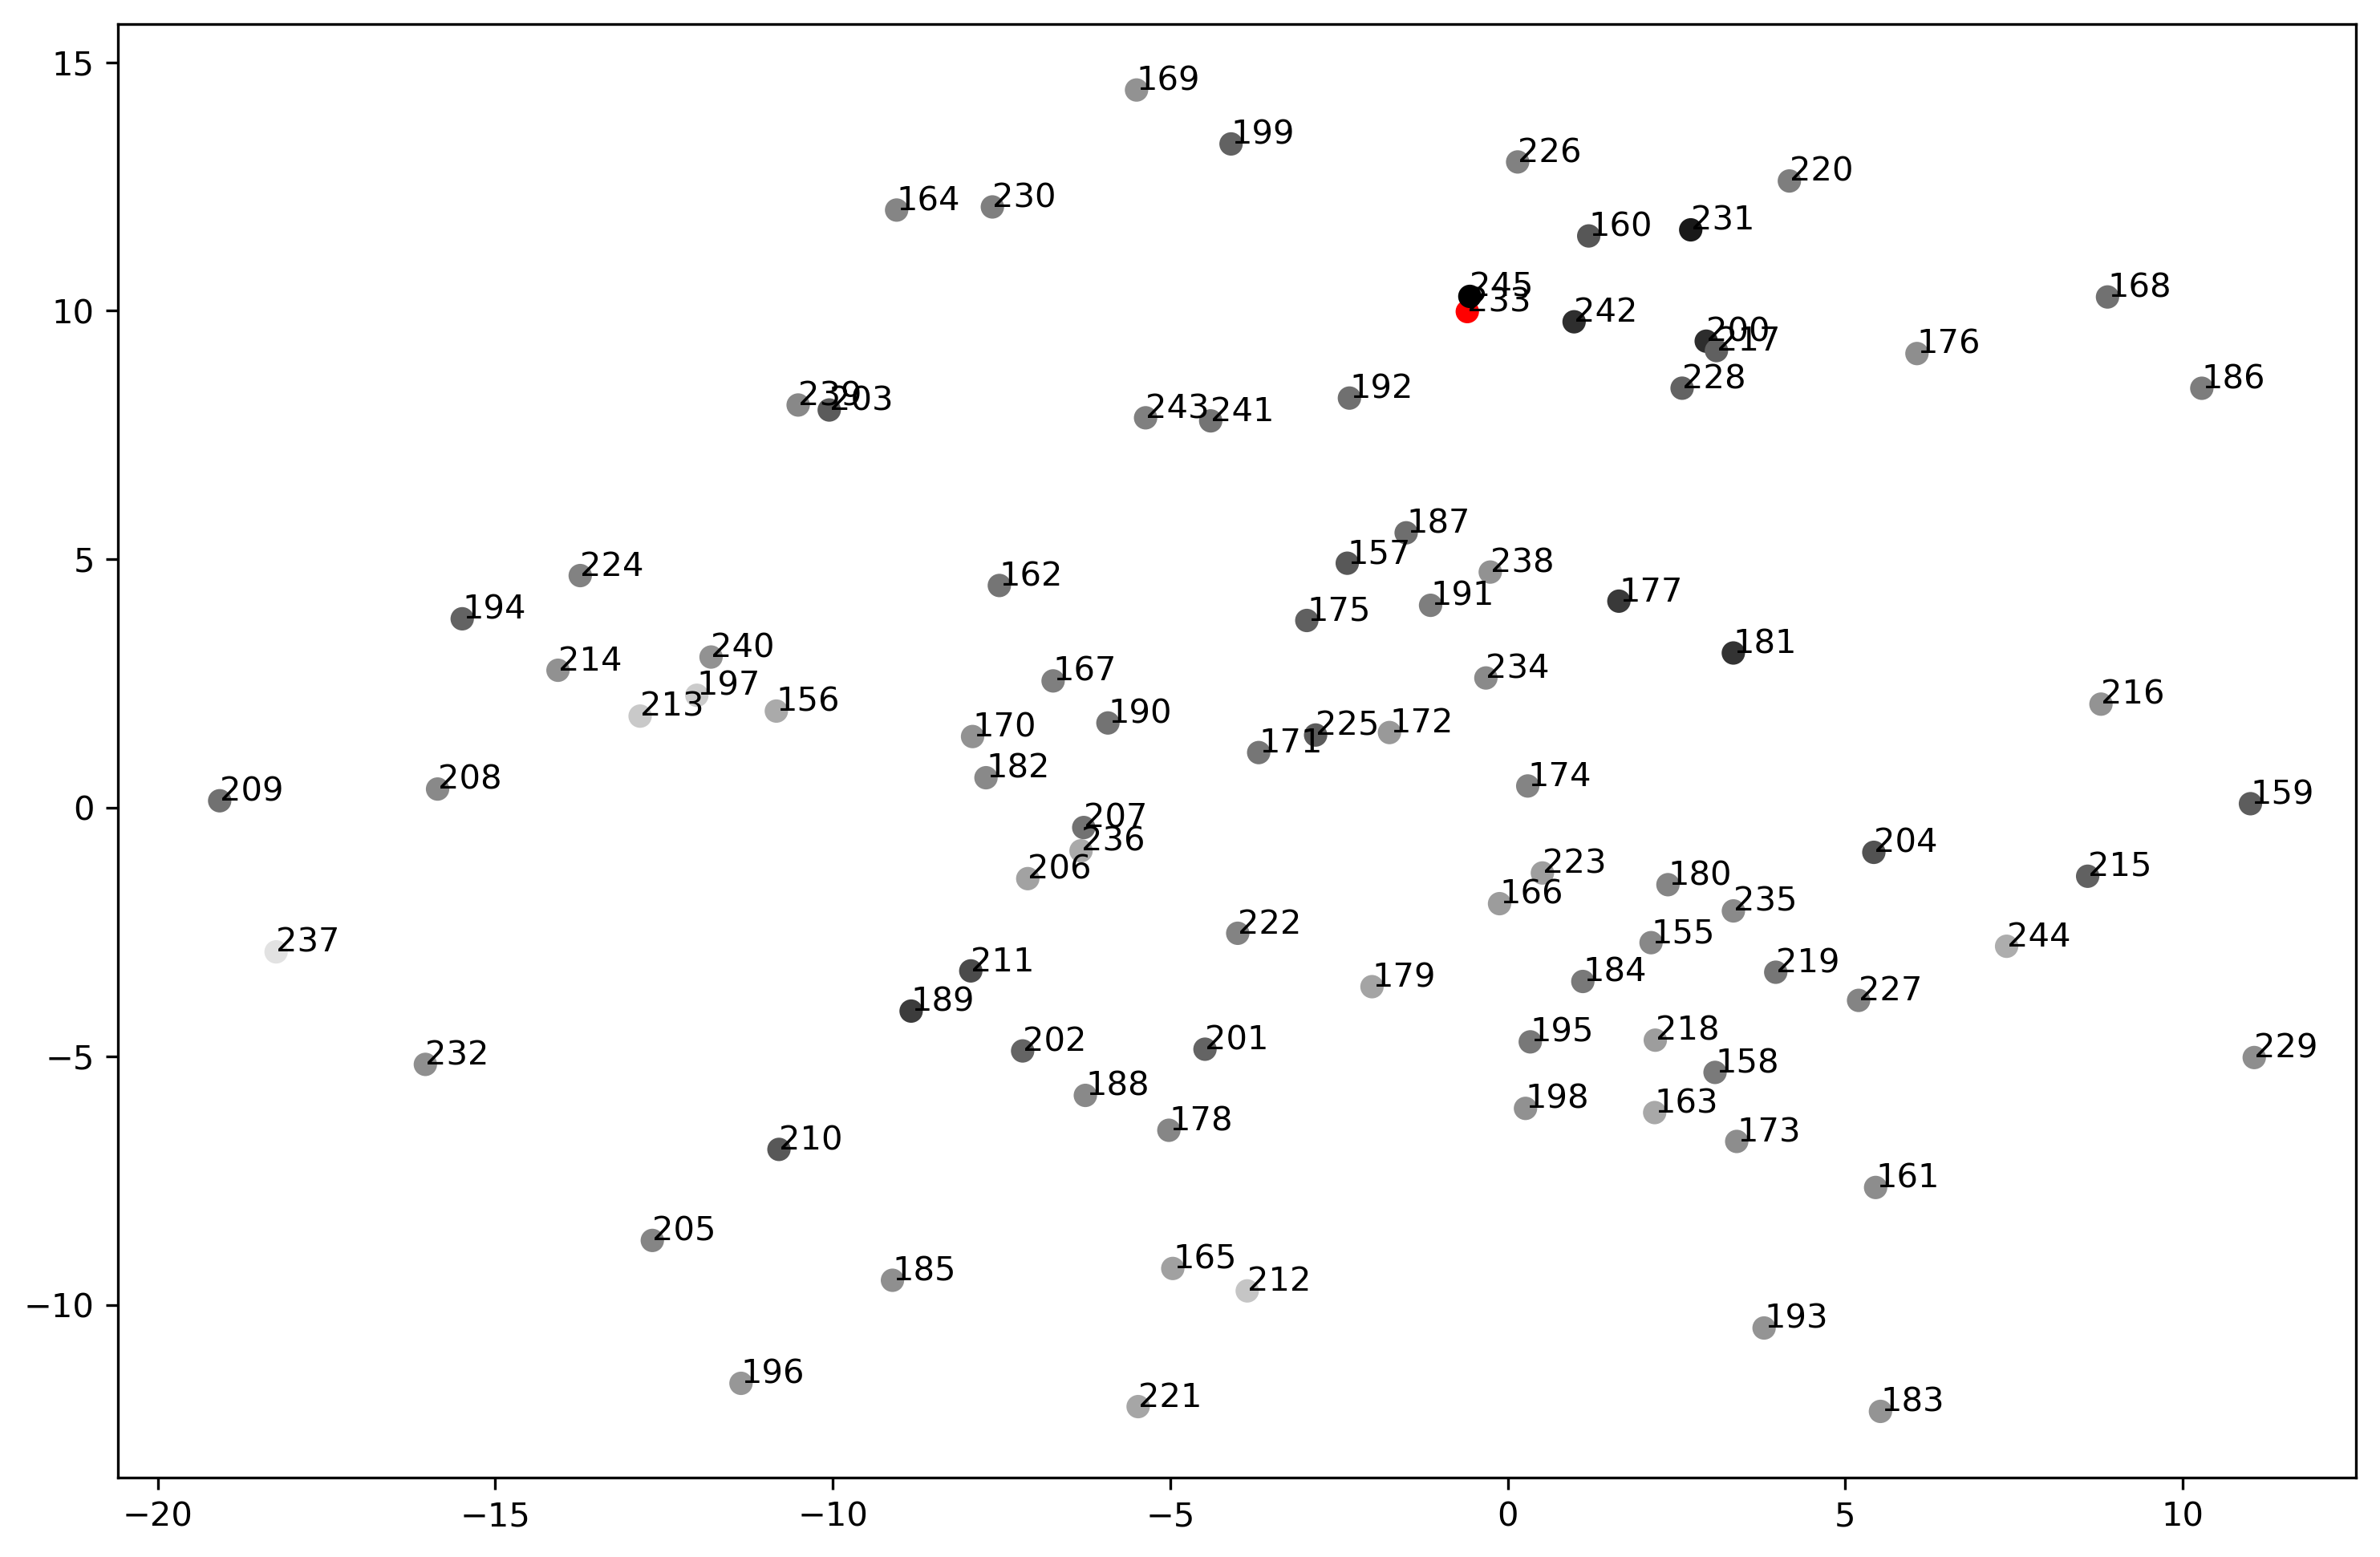
\includegraphics[width=\textwidth]{images/road_tsne.png}
    \caption{Road embedding points after t-SNE dimensionality reduction.}
    \label{fig: road_correlation_tsne}
\end{figure}

Next, starting from road embedding matrix $E$, we perform t-SNE\cite{tsne} algorithm to reduce the embedding dimension from $d_r=64$ to $2$, and plot the points on a 2-D figure. The color of each road remains same as figure \ref{fig: road_correlation_map}, where the red point still stands for $r_{233}$. If $C$ is able to represent the road correlations, then the high-correlated roads mentioned above should be close to the red point. As shown in figure \ref{fig: road_correlation_tsne}, the points for $r_{245}, r_{242}, r_{231}, r_{200}, r_{177}, r_{181}$ are near to $r_{233}$, which means $C$ is able to represent the similarity between road embedding vectors, i.e. road correlation.

In conclusion, these two case experiments prove not only the rationality of our thesis on \textit{trajectory-based road correlation}, but also the effectiveness of our proposed model and methods.


\section{Conclusion and Future Work}
This is conclusion.\clearpage

\参考文献
  \printbibliography[heading=none]\clearpage
\致谢
  
This paper is funded by myself (Grant No. DZ-2000-2022). First, I would like to thank my parents who are the actual funders of this work, as well as my life. Secondly, thank all the teachers and students in SUSTech-UTokyo Joint Research Center for their assistance both in academic and in life, especially Prof. Xuan Song, Dr. Quanjun Chen and Dr. Renhe Jiang. I also have to express my sincere gratitude to my dear 10-year brothers Yulong Huang, Yu Xing, Zihao Xia and Tianxing Lv, for accompanying me on the road of chasing my dreams. Then, thanks my roommates Yangchenguang Liu, Yueqian Hu and Liangchen Fang, for our four years of happy times together. Finally, thank the other four team members in our CUILab team: Yusong Cui, Yuchen Wang, Haotian Gao and Yifan Zhao. Wish all of you a prosperous future.

Thanks to everyone who helped me, supported me, and cared about me. ``To your valour, my sword, and our victory together. Long may the Sun shine!''

\vspace{\baselineskip}

The \LaTeX template of this paper can be found at \href{https://github.com/iydon/sustechthesis}{github.com/iydon/sustechthesis}.
\end{document}